%% Dokumentklasse KOMA-Script Report
\documentclass[paper=a4, 12pt]{scrreprt}
%% Encoding UTF8
\usepackage[utf8]{inputenc}
%%Use Source Sans Pro Textstyle
\usepackage[default]{sourcesanspro}
%% 8 Bit Aufloesung der Buchstaben
\usepackage[T1]{fontenc}
%% Seitenraender
%\usepackage[scale=0.72]{geometry}
\usepackage[scale=0.72, twoside, bindingoffset=2mm]{geometry}
%% Spracheinstellungen
\usepackage[english, naustrian]{babel} % your native language must be the last one!!
%% erweiterte Farbenpalette
\usepackage[dvipsnames]{xcolor}
%% Abbildungen
\usepackage{graphicx}
%%Tabelen mit Farbe (cellcolor)
\usepackage{tabulary}
\usepackage{colortbl}
\usepackage{colortbl}
\usepackage{subcaption}
\PassOptionsToPackage{dvipsnames,svgnames,table}{xcolor}
%% Tabellen (erweitert)
\usepackage{tabularx}
%% TikZ + Circuit-TikZ (fuer Schaltungen)
\usepackage[europeanresistors, europeaninductors]{circuitikz}
%% Nuetzliche TikZ Libraries
\usetikzlibrary{arrows, automata, positioning}
%% mathematik
\usepackage{amsmath, amssymb}
%%Formelbeschreibung
\newenvironment{conditions}
  {\par\vspace{\abovedisplayskip}\noindent\begin{tabular}{>{$}l<{$} @{${}...{}$} l}}
  {\end{tabular}\par\vspace{\belowdisplayskip}}
%\usepackage{mathtools}	
%% pdf-einbindung
\usepackage{pdfpages}
%% scource-code einbindung
\usepackage{listings, scrhack} %scrhack vermeidet Umschaltung auf KOMA
% Floats..
\usepackage{courier}
%% euro-symbol
\usepackage{eurosym}
%% landcsape-seiten ermöglichen
\usepackage{lscape}

%% Diplomarbeits-Format
\usepackage{srdpdipa}

%% Abkuerzungsverzeichnis
\usepackage[]{acronym}

%% Todos
\usepackage[]{todonotes}

%% Ganttdiagramme
\usepackage{pgfgantt}

%% Subfigures
\usepackage[lofdepth]{subfig}

%% Set the counter for the 2.1.1 latex how to get 2.1.1.1
\setcounter{secnumdepth}{4}

%% Für Quellenangaben unter Bildern
\newcommand*{\quelle}[1]{\par\raggedleft\footnotesize Quelle:~#1}

% add the rotating package
\usepackage{rotating}

%

\usepackage{subcaption}

\usepackage{enumitem}



% ???
\usepackage{wrapfig}

%% Listings (Code)
\usepackage{listings}
\usepackage{color}




%% TypeScript

\usepackage[utf8]{inputenc}
\usepackage{xcolor}
\usepackage{listings}

% ---------------------------
% TSX Language and Style Setup
% ---------------------------
\lstdefinelanguage{TSX}{
  sensitive=true,
  keywords={
    import, from, class, extends, function, return, if, else, for, while,
    const, let, var, type, interface, implements, private, public, protected,
    static, any, never, boolean, string, number, unknown, readonly, this, new,
    React, JSX
  },
  morecomment=[l]{//},         % single-line comments
  morecomment=[s]{/*}{*/},     % multi-line comments
  morestring=[b]",             % "strings"
  morestring=[b]',             % 'strings'
  alsoletter={:,<,>,/},        % treat these characters as part of words
  % Color angle brackets (and closing tags) in a different color
  moredelim=[s][\color{blue}]{<}{>},
  moredelim=[s][\color{blue}]{</}{>},
}

\lstdefinestyle{mytsx}{
  language=TSX,
  backgroundcolor=\color{white},      % White background
  basicstyle=\ttfamily\small,         % Monospaced, small font
  keywordstyle=\color{blue}\bfseries,
  stringstyle=\color{orange},
  commentstyle=\color{gray}\itshape,
  frame=single,                       % Frame around the code
  numbers=left,                       % Line numbers on the left
  breaklines=true,
  columns=fullflexible
}

% ---------------------------
% JSON Language and Style Setup
% ---------------------------
\lstdefinelanguage{json}{
  basicstyle=\ttfamily\small,
  numbers=none,
  breaklines=true,
  frame=single,
  backgroundcolor=\color{white},
  % Color numbers and punctuation using literate programming:
  literate=
    {0}{{{\color{orange}0}}}{1}
    {1}{{{\color{orange}1}}}{1}
    {2}{{{\color{orange}2}}}{1}
    {3}{{{\color{orange}3}}}{1}
    {4}{{{\color{orange}4}}}{1}
    {5}{{{\color{orange}5}}}{1}
    {6}{{{\color{orange}6}}}{1}
    {7}{{{\color{orange}7}}}{1}
    {8}{{{\color{orange}8}}}{1}
    {9}{{{\color{orange}9}}}{1}
    {:}{{{\color{blue}{:}}}}{1}
    {,}{{{\color{blue}{,}}}}{1}
    {\{}{{{\color{red}{\{}}}}{1}
    {\}}{{{\color{red}{\}}}}}{1}
    {[}{{{\color{red}{[}}}}{1}
    {]}{{{\color{red}{]}}}}{1}
}

\lstdefinestyle{myjson}{
  language=json,
  backgroundcolor=\color{white},
  basicstyle=\ttfamily\small,
  frame=single,
  numbers=left,         % Optional: add line numbers if you want
  breaklines=true,
  columns=fullflexible
}




\lstdefinestyle{mysql}{
  language=SQL,                      % SQL als Sprache auswählen
  backgroundcolor=\color{white},     % Weißer Hintergrund
  basicstyle=\ttfamily\small,        % Monospace-Schrift in kleiner Größe
  keywordstyle=\color{blue}\bfseries, % Schlüsselwörter in Blau und fett
  stringstyle=\color{orange},         % Zeichenketten in Orange
  commentstyle=\color{gray}\itshape,  % Kommentare in Grau und kursiv
  frame=single,                      % Rahmen um den Code
  numbers=left,                      % Zeilennummern links
  breaklines=true,                   % Zeilenumbrüche aktivieren
  columns=fullflexible
}

\lstdefinestyle{mytsx}{
  language=TSX,
  backgroundcolor=\color{white},      % White background
  basicstyle=\ttfamily\small,         % Monospaced, small font
  keywordstyle=\color{blue}\bfseries,
  stringstyle=\color{orange},
  commentstyle=\color{gray}\itshape,
  frame=single,                       % Frame around the code
  numbers=left,                       % Line numbers on the left
  breaklines=true,
  columns=fullflexible
}

\lstdefinelanguage{myurl}{
    morestring=[b]",
    morecomment=[l]{//},
    morekeywords={domainname, dashboard, department, class, device}
}


\lstdefinestyle{myconsole}{
  language=bash,                      % Syntax highlighting for bash
  backgroundcolor=\color{white},      % White background
  basicstyle=\ttfamily\small,         % Monospaced, small font
  keywordstyle=\color{black}\bfseries, % Commands in bold black
  stringstyle=\color{green},          % Strings in green
  commentstyle=\color{gray}\itshape,  % Comments in gray italic
  frame=single,                       % Frame around the code
  numbers=left,                       % Line numbers on the left
  breaklines=true,
  columns=fullflexible
}










\definecolor{dkgreen}{rgb}{0,0.6,0}
\definecolor{gray}{rgb}{0.5,0.5,0.5}
\definecolor{mauve}{rgb}{0.58,0,0.82}

\lstset{frame=none,
  language=Python,
  aboveskip=3mm,
  belowskip=3mm,
  showstringspaces=false,
  columns=flexible,
  basicstyle={\small\ttfamily},
  numbers=left,
  numberstyle=\tiny\color{gray},
  keywordstyle=\color{blue},
  commentstyle=\color{dkgreen},
  stringstyle=\color{mauve},
  breaklines=true,
  breakatwhitespace=true,
  tabsize=3
}

\lstset{literate=%
  {Ö}{{\"O}}1
  {Ä}{{\"A}}1
  {Ü}{{\"U}}1
  {ß}{{\ss}}1
  {ü}{{\"u}}1
  {ä}{{\"a}}1
  {ö}{{\"o}}1
}

\usepackage{longtable}

%% TIKZ Flowcharts
\usepackage{tikz}
\usetikzlibrary{shapes.geometric, arrows}

\tikzstyle{startstop} = [rectangle, rounded corners, minimum width=3cm, minimum height=1cm,text centered, draw=black, fill=green!32]
\tikzstyle{io} = [trapezium, trapezium left angle=70, trapezium right angle=110, minimum width=3cm, minimum height=1cm, text centered, draw=black, fill=red!35]
\tikzstyle{process} = [rectangle, minimum width=3cm, minimum height=1cm, text centered, draw=black, fill=cyan!32]
\tikzstyle{decision} = [diamond, minimum width=3cm, minimum height=1cm, text centered, draw=black, fill=orange!42]

\tikzstyle{arrow} = [thick,->,>=stealth]


%% definitionen =====================================%%
\dataSchool{HTBLuVA St. Pölten}
\dataDepartment{Höhere Lehranstalt für Elektronik und Technische Informatik}
\dataSubdepartment{Ausbildungsschwerpunkte Embedded- \& Wireless Systems}
\dataSession{2024/25}


\title{AirSens Classroom Data Capturing}
\author{Thomas Potzmader \and Tobias Geppl}
\date{4. April 2025}
\place{St. P\"olten}
\professor{Dipl.-Ing. Wolfgang Uriel Kuran \and DI (FH) Johannes Tomitsch}



%%====================================================%%

% Hyperlinks im Dokument
\usepackage[colorlinks=true,
    linkcolor=black,
    citecolor=black,
    bookmarks=true,
    urlcolor=black,
    bookmarksopen=true]{hyperref}

\begin{document}

\frontmatter

%% titelseite ==========================================%%
\maketitle
%%======================================================%%

%% komplett leere seite ================================%%
\newpage\null\thispagestyle{empty}%\newpage
%%======================================================%%

%% eidesstattliche erklärung ===========================%%
\begin{affidavit}
    \unterschrift{Thomas Potzmader}
    \unterschrift{Tobias Geppl}
\end{affidavit}
%%======================================================%%

%% dokumentation (deutsch/englisch) ====================%%
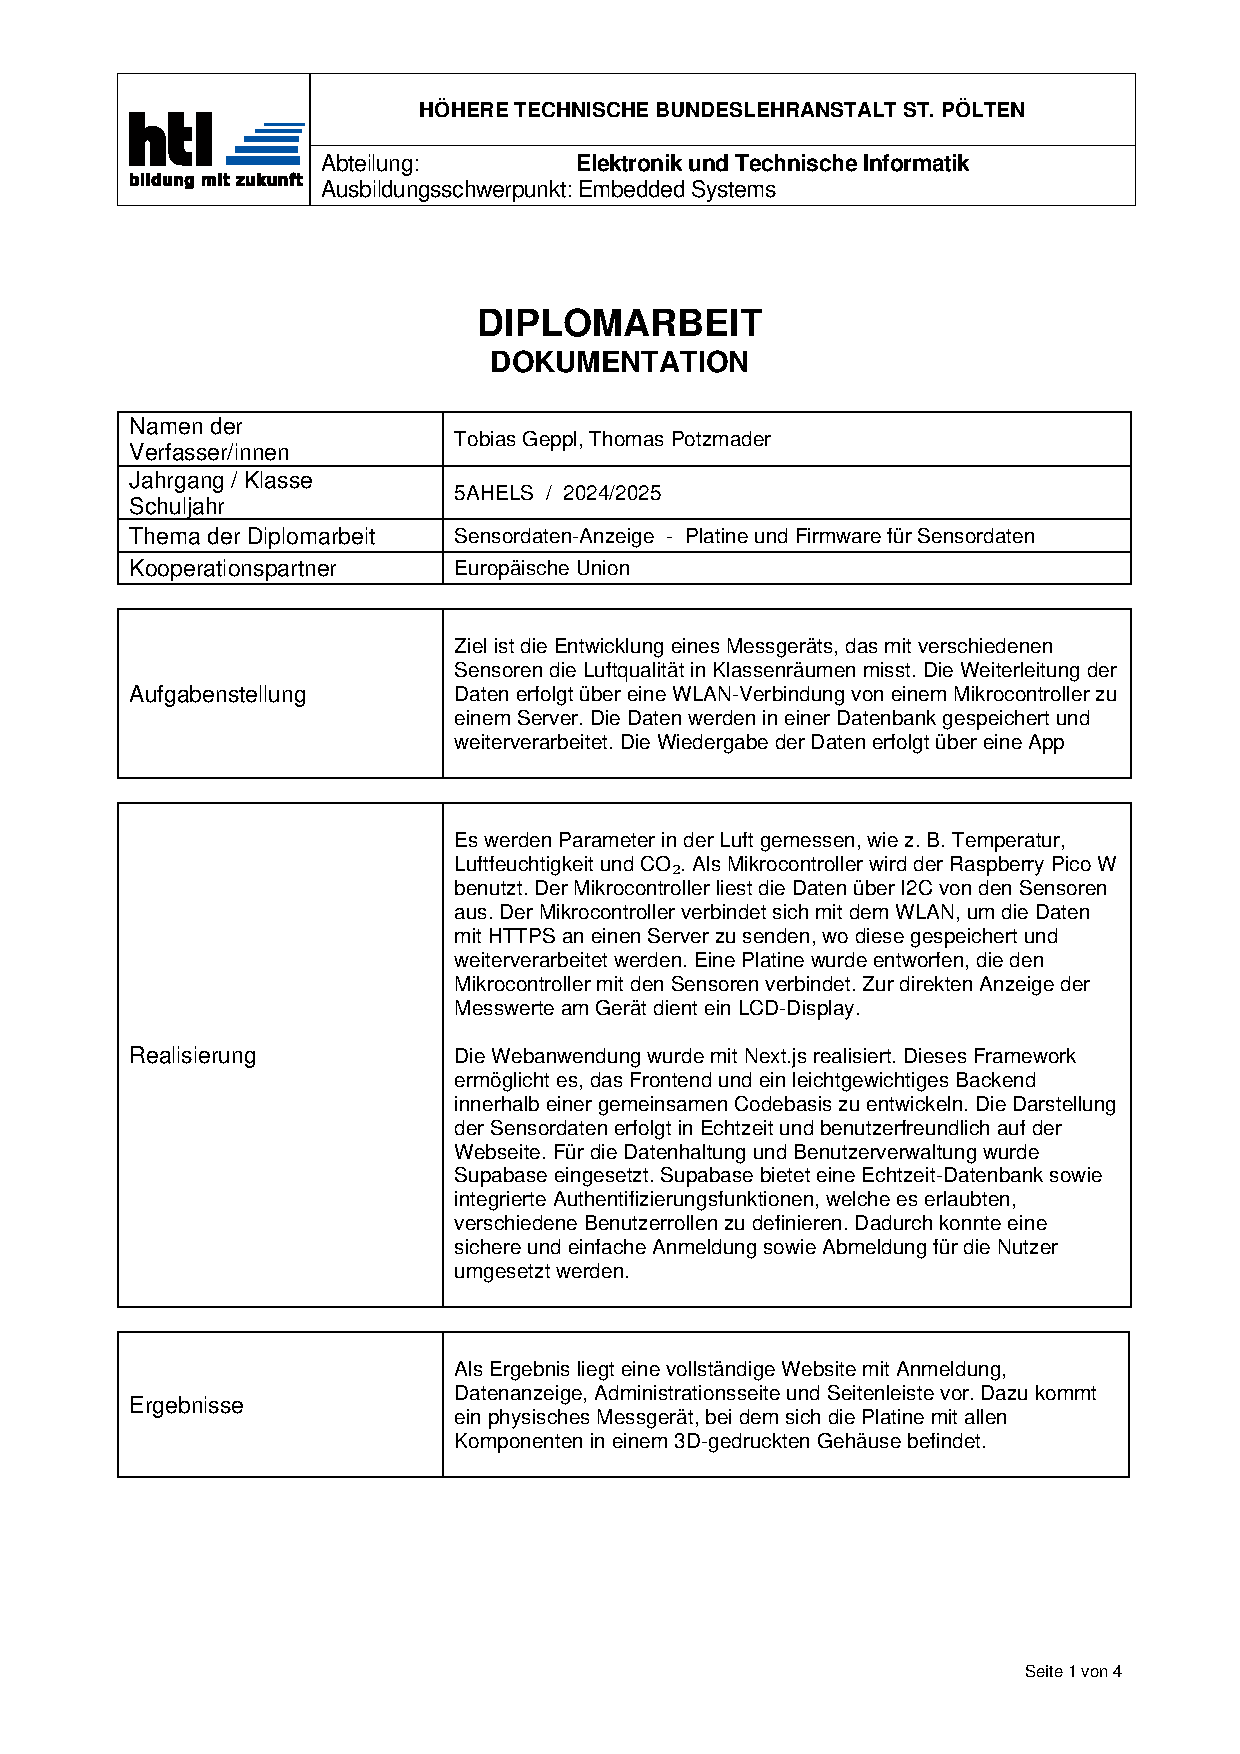
\includepdf[pages=1-4]{doc/pdfs/E_DiplArbeit_Seite_4_5_new.pdf}                 %Dokumentation(PDF) einfügen
%%\includepdf[pages=-]{doc/pdfs/dokumentation-en.pdf}                 %Dokumentation(PDF) einfügen
%%======================================================%%

\cleardoublepage                                              %Seite freilassen


%% diplomantenvorstellung ==============================%%
%%\includepdf[pages=-]{doc/pdfs/Tobias.pdf}                          %Vorstellung(PDF) einfügen
%%\cleardoublepage                                              %Seite freilassen
%%\includepdf[pages=-]{doc/pdfs/Thomas.pdf}                          %Vorstellung(PDF) einfügen
%%\begin{inhalt}
\clearpage
\thispagestyle{empty} % nur für die erste Seite
\begin{center}

\dataSchool{HTBLuVA St. Pölten}
\dataDepartment{Höhere Lehranstalt für Elektronik und Technische Informatik}
\dataSubdepartment{Ausbildungsschwerpunkte Embedded- \& Wireless Systems}
\dataSession{2024/25}


\begin{center}
    \vspace*{-15mm}
    \begin{minipage}[t]{\textwidth}
        \begin{minipage}[c]{0.1\textwidth}
            \hspace*{-5mm}
            
\includegraphics[width=1.5\linewidth]{doc/img/htl.png}
        \end{minipage}%
        \begin{minipage}[c]{0.8\textwidth}
            \centering
            {\bfseries\sffamily\large HTBLuVA St. Pölten}\\
            \vspace{1.5mm}
            {\bfseries\sffamily\small Höhere Lehranstalt für Elektronik und Technische Informatik}\\
            \vspace{1.5mm}
            {\sffamily\scriptsize Ausbildungsschwerpunkte Embedded- \& Wireless Systems}\\
            \vspace{1.5mm}
        \end{minipage}%
        \begin{minipage}[c]{0.1\textwidth}
            \hspace*{-2mm}
            
\includegraphics[width=1.5\linewidth]{doc/img/htl-bbs.png}
        \end{minipage}
    \end{minipage}
    \rule{\textwidth}{0.2pt}
    \vspace{0.5cm}

    {\LARGE \textbf{DIPLOMARBEIT}}\\
    {\large \textbf{DOKUMENTATION}}
\end{center}

\vspace{1cm}

\begin{tabular}{|p{5cm}|p{10cm}|}
    \hline
    \textbf{Namen der Verfasser/innen} & Tobias Geppel, Thomas Potzmader \\
    \hline
    \textbf{Jahrgang / Klasse} & \href{https://www.htlstp.ac.at}{5AHETLS} / 2024/2025 \\
    \hline
    \textbf{Thema der Diplomarbeit} & Sensordaten-Anzeige – Platine und Firmware für Sensordaten \\
    \hline
    \textbf{Kooperationspartner} & Europäische Union \\
    \hline
    \textbf{Aufgabenstellung} & Ziel ist die Entwicklung eines Messgeräts, das mit verschiedenen Sensoren die Luftqualität in Klassenräumen misst. Die Daten werden über eine WLAN-Verbindung von einem Mikrocontroller an einen Server übertragen. Dort werden sie gespeichert und weiterverarbeitet. Die Anzeige der Daten erfolgt über eine App. \\
    \hline
    \textbf{Realisierung} & Es werden Parameter wie Temperatur, Luftfeuchtigkeit und CO$_2$-Konzentration gemessen. Als Mikrocontroller wird der Raspberry Pi Pico W eingesetzt. Die Sensoren kommunizieren über I2C mit dem Mikrocontroller. Dieser verbindet sich per WLAN und sendet die Daten über HTTPS an einen Server, wo sie gespeichert und weiterverarbeitet werden.

    Zusätzlich wurde eine Platine entworfen, welche den Mikrocontroller mit den Sensoren verbindet. Ein LCD-Display dient zur direkten Anzeige der Messwerte am Gerät.

    Die Webanwendung wurde mit dem Framework Next.js entwickelt. Damit konnte sowohl das Frontend- als auch ein leichtgewichtiges Backend innerhalb einer gemeinsamen Codebasis realisiert werden. Die Sensordaten werden in Echtzeit und benutzerfreundlich auf der Webseite dargestellt. Für die Datenhaltung und Benutzerverwaltung kommt Supabase zum Einsatz. Supabase bietet eine Echtzeit-Datenbank und integrierte Authentifizierungsfunktionen, wodurch unterschiedliche Benutzerrollen definiert werden können. Dadurch wurde eine sichere und einfache Anmeldung sowie Abmeldung für die Nutzer realisiert. \\
    \hline
    \textbf{Ergebnisse} & Das Ergebnis umfasst eine vollständige Website mit Anmeldung, Datenanzeige, Administrationsseite und Seitenleiste. Zusätzlich wurde ein physisches Messgerät entwickelt, bei dem sich die Platine mit allen Komponenten in einem 3D-gedruckten Gehäuse befindet. \\
    \hline
\end{tabular}
\end{center}
\end{inhalt}

  

%%======================================================%%

%%\cleardoublepage                                              %Seite freilassen

%% danksagung ==========================================%%
\begin{acknowledgements}
\subsubsection*{Name 1}
Danksagung Inhalt
\\
Danke Danke Danke Danke Danke Danke Danke Danke Danke Danke Danke Danke Danke Danke Danke Danke 
\\                              %Absatz
\subsubsection*{Name 2}
Danksagung Inhalt
\\
Danke Danke Danke Danke Danke Danke Danke Danke Danke Danke Danke Danke Danke Danke 
\end{acknowledgements}
                             
%%======================================================%%

\cleardoublepage                                              %Seite freilassen

%% inhaltsverzeichnis ==================================%%
\renewcommand*\chapterpagestyle{scrheadings}
\tableofcontents
%%======================================================%%

%%\cleardoublepage                                              %Seite freilassen

%% HAUPTTEIL ===========================================%%
\responsible{Thomas Potzmader, Tobias Geppl} 
\mainmatter

%Chapter 1 - Einführung/Einleitung
\responsible{Thomas Potzmader, Tobias Geppl} 
\begin{inhalt}
\renewcommand*\chapterpagestyle{scrheadings}
\chapter{Einleitung}
Zielsetzung Aufgabenstellung des Gesamtprojekts

Individuelle Zielsetzung und Aufgabenstellung



\section{Section}
Inhalt

\begin{figure}[!htb]
\centering
\includegraphics[width=0.75\textwidth]{img/Quest1.jpg}
\caption[Bildbezeichnung für Abbildungsverzeichnis]{Bildunterschrift}
\label{labelname}
\end{figure}

Inhalt 2

\end{inhalt}                                     %Einführung(LaTeX File) einfügen

%Chapter 2 - (Grundlagen & Methoden)
\responsible{Thomas Potzmader, Tobias Geppl} 

\begin{inhalt}
\chapter{Grundlagen \& Methoden}
\renewcommand*\chapterpagestyle{scrheadings}
 \section{Hardwaredesign \& Programmierung}
 
\subsection{Altium Designer}

Altium Designer ist eine kostenpflichtige Software von Autodesk für die Entwicklung und das Design von PCBs (Printed Circuit Boards). Die Software bietet eine komplette Entwicklungsumgebung für die Erstellung von elektronischen Schaltungen. Sie bietet unter anderem Schaltungsdesign, Schaltkreissimulationen und physisches PCB-Design. 
 \cite{AltiumDesignerWiki}

\subsection{I2C}

I2C (Inter-Integrated-Circuit) ist ein synchrones Bussystem basierend auf dem Master-Slave-Prinzip zur Datenübertragung zwischen Peripheriegeräten. Es benutzt eine Daten- sowie eine Taktleitung und wird bei Geräten mit geringem Abstand zueinander eingesetzt. 
 \cite{I2CKommunikation}

\subsection{SPI}

SPI (Serial Peripheral Interface) ist ein synchrones Bussystem basierend auf dem Master-Slave-Prinzip. Es benutzt 4 Leitungen, davon eine Taktleitung, eine Slave-Select-Leitung und 2 Datenleitungen. Durch die 2 Datenleitungen (Master In Slave Out, Master Out Slave In) ist dieses Bussystem vollduplexfähig. \cite{SPI_Kommunikation}

\subsection{HTTPS} \label{sec:HTTPS-Grundlagen}

HTTPS (Hypertext Transfer Protocol Secure) ist ein Protokoll zur Übertragung von Daten zwischen Webservern und Webbrowsern. HTTPS unterscheidet sich von HTTP durch zusätzliche Verschlüsselung mittels SSL/TLS. \cite{HTTPS_Kommunikation}

\subsection{Visual Studio Code} \label{sec:VS-Code}

Visual Studio Code ist ein kostenloser Text-Editor der Firma Microsoft. Er ist sehr umfangreich durch viele Erweiterungsmöglichkeiten und wird für viele verschiedene Anwendungen eingesetzt. Visual Studio Code bietet eine moderne und individuell anpassbare Benutzeroberfläche. \cite{VisualStudioCode}

\subsection{Raspberry PI Pico Erweiterung} \label{sec:PicoExtension}

Die Raspberry Pi Pico Erweiterung ist eine Erweiterung in Visual Studio Code, die das Programmieren von RP2040-Mikrocontroller-Boards in C/C++ vereinfacht. Sie bietet Projektverwaltung sowie Automatisierung typischer Schritte wie das Einrichten des Pico SDK, die Compiler-Einstellungen oder das Laden der Firmware auf das Board. \cite{Raspberry_Pi_Pico_Erweiterung}


\end{inhalt}  
\begin{inhalt}
\chapter{Grundlagen \& Methoden}
\renewcommand*\chapterpagestyle{scrheadings}

Verwendete Technologien 
\section{Web Entwicklung}

Web-Entwicklung \cite{WebEntwicklungWiki} bezeichnet die Erstellung und Gestaltung von Websites und Webanwendungen, die über das Internet zugänglich sind. Dabei werden verschiedene Technologien und Programmiersprachen genutzt, um Inhalte darzustellen, interaktive Funktionen bereitzustellen und Daten zu verarbeiten. Eine Website besteht typischerweise aus dem Frontend, die dem Nutzer präsentiert wird, sowie einen Backend, die im Hintergrund abläuft und beispielsweise Daten verarbeitet oder speichert. Dabei kommen moderne Frameworks und Entwicklungsumgebungen zum Einsatz, um eine effiziente und ansprechende Umsetzung zu ermöglichen. 

\subsection{Frontend} 

Das Frontend \cite{WebEntwicklungFrontendWiki} umfasst alle Komponenten einer Website oder Webanwendung, die direkt mit dem Nutzer interagieren. Es stellt die visuelle und funktionale Oberfläche bereit, über die Inhalte dargestellt und Aktionen durchgeführt werden können. Typische Technologien im Frontend-Bereich sind HTML, CSS und JavaScript. Moderne Frameworks wie React, Angular oder Vue.js ermöglichen dabei die Erstellung dynamischer und reaktionsschneller Benutzeroberflächen. Das Ziel des Frontends ist es, ein ansprechendes, intuitives und barrierefreies Nutzererlebnis zu gewährleisten. Dabei spielen Aspekte wie responsives Design, Performance und Zugänglichkeit eine wesentliche Rolle. Das Frontend, wird in den Kapiteln bis 2.1.6 beschrieben. 

\subsection{Backend}

Das Backend \cite{WebEntwicklungFrontendBackendWiki} bildet das Rückgrat einer Webanwendung und arbeitet im Hintergrund, um Daten zu verarbeiten, Geschäftslogik umzusetzen und Verbindungen zu Datenbanken herzustellen. Es ist nicht direkt für den Endnutzer sichtbar, sorgt jedoch dafür, dass alle Funktionen einer Website reibungslos ablaufen. Gängige Programmiersprachen und Frameworks im Backend-Bereich sind unter anderem PHP, Python, Ruby, Java, Node.js oder .NET. Die Aufgaben des Backends umfassen unter anderem Authentifizierung, Autorisierung, API-Entwicklung, Datenverwaltung und Sicherheitsaspekte. Durch die enge Zusammenarbeit mit dem Frontend wird eine nahtlose Integration und effiziente Datenübertragung zwischen Client und Server gewährleistet.

\subsection{Datenbank}

Eine Datenbank \cite{DatenBankWiki} bildet das zentrale Element zur Speicherung, Verwaltung und Abfrage von Daten innerhalb einer Webanwendung. Sie ermöglicht es, Informationen strukturiert abzulegen und bei Bedarf effizient abzurufen oder zu aktualisieren. Dabei wird oft zwischen relationalen Datenbanken, wie MySQL, PostgreSQL oder Oracle, und NoSQL-Datenbanken, wie MongoDB oder Cassandra, unterschieden. Relationale Datenbanken nutzen Tabellen und vordefinierte Beziehungen, um Daten zu organisieren, während NoSQL-Datenbanken flexiblere Datenmodelle bieten, die insbesondere bei großen, unstrukturierten Datenmengen Vorteile bieten können. Durch die enge Integration der Datenbank mit dem Backend wird sichergestellt, dass die Webanwendung zuverlässig und performant auf die benötigten Daten zugreifen kann.

\subsection{Next.js}
Next.js \cite{NextJSWiki} ist ein modernes Framework für die Entwicklung von React-Anwendungen, das sowohl serverseitiges Rendering als auch statische Seitengenerierung unterstützt. Durch diese Funktionen können Entwickler performante und SEO-freundliche Webanwendungen erstellen. Next.js vereinfacht die Handhabung von Routing, API-Routen und anderen komplexen Aufgaben, indem es eine klare und strukturierte Entwicklungsumgebung bietet. Dies führt zu einer verbesserten Entwicklererfahrung und ermöglicht die effiziente Erstellung skalierbarer Webprojekte.

\subsection{ReactWiki}
React \cite{ReactWiki} ist eine JavaScript-Bibliothek zur Erstellung von Benutzeroberflächen, die es Entwicklern ermöglicht, wiederverwendbare UI-Komponenten zu erstellen. Es bildet die Grundlage für Next.js und konzentriert sich darauf, den Zustand und die Darstellung von Komponenten effizient zu verwalten. Durch das deklarative Programmiermodell wird die Entwicklung von interaktiven Anwendungen vereinfacht, während gleichzeitig eine hohe Performance und Skalierbarkeit gewährleistet werden kann.

\subsection{TypescriptWiki}
Typescript \cite{TypescriptWiki} erweitert JavaScript um statische Typisierung und andere Features, die die Codequalität und Wartbarkeit von Anwendungen verbessern. Durch die frühzeitige Erkennung von Fehlern im Code und die Unterstützung moderner JavaScript-Funktionalitäten bietet Typescript eine solide Basis für die Entwicklung von robusten und fehlerarmen Anwendungen. Viele moderne Frameworks, darunter auch Next.js, profitieren von den zusätzlichen Sicherheitsmechanismen und der besseren Entwicklerunterstützung, die Typescript bietet.

\subsection{TailwindWiki}
Tailwind \cite{TailwindWiki} ist ein Utility-first CSS-Framework, das es ermöglicht, direkt im Markup stilisierte Komponenten zu erstellen. Anstatt vordefinierte Komponenten zu nutzen, bietet Tailwind eine umfangreiche Sammlung an Klassen, die individuell kombiniert werden können, um maßgeschneiderte Designs zu realisieren. Dies führt zu einem flexiblen und effizienten Styling-Prozess, bei dem Entwickler schnell und ohne umfangreiche CSS-Dateien arbeiten können. Tailwind unterstützt dabei die Erstellung von responsiven und modernen Benutzeroberflächen, die sich leicht an unterschiedliche Designanforderungen anpassen lassen.

\subsection{ShadCN}
ShadCN \cite{ShadCN} ist eine moderne UI-Komponentenbibliothek, die speziell für die Erstellung ansprechender und konsistenter Benutzeroberflächen entwickelt wurde. Sie integriert sich nahtlos in moderne Frontend-Frameworks und bietet eine Vielzahl von wiederverwendbaren Komponenten, die den Entwicklungsprozess beschleunigen und die Wartbarkeit der Anwendungen verbessern.


\subsection{Zustand} \label{subsec:Zustand} 
Zustand \cite{Zustand} ist ein leichtgewichtiges und flexibles State-Management-Tool für React-Anwendungen, das sich auf die Nutzung von Hooks stützt. Es ermöglicht Entwicklern, globale Zustände einfach zu definieren und zu verwalten, ohne dabei auf komplexe Provider- oder Context-Modelle zurückgreifen zu müssen. Durch den Verzicht auf übermäßigen Boilerplate-Code und die intuitive API bietet Zustand eine effiziente Alternative zu anderen State-Management-Lösungen. Die Bibliothek zeichnet sich durch ihre hohe Performance und einfache Skalierbarkeit aus, was sie besonders attraktiv für moderne, dynamische Webanwendungen macht.

\subsection{Zod}
\label{subsec:Zod}
Zod \cite{Zod} ist eine TypeScript-orientierte Validierungsbibliothek, die es ermöglicht, Datenstrukturen präzise zu definieren und zur Laufzeit zu überprüfen. Durch die Nutzung von Zod können Entwickler sicherstellen, dass ihre Anwendungen robust gegenüber fehlerhaften oder unerwarteten Daten sind, was die Zuverlässigkeit und Wartbarkeit des Codes erheblich verbessert.

\subsection{Supabase}
Supabase \cite{Supabase} ist eine umfassende Backend-as-a-Service-Plattform, die Entwicklern eine Alternative zu traditionellen Backend-Lösungen bietet. Sie kombiniert mehrere Funktionen, die eine schnelle und sichere Entwicklung von Webanwendungen ermöglichen.

\subsubsection{Supabase DB}
Die Supabase DB \cite{SupabaseDB} basiert auf PostgreSQL und bietet eine skalierbare und leistungsfähige relationale Datenbanklösung. Sie ermöglicht die Speicherung, Abfrage und Verwaltung von Daten in Echtzeit und ist dabei vollständig in die Supabase-Plattform integriert, um eine reibungslose Datenverwaltung zu gewährleisten.

\subsubsection{Supabase Auth}
Supabase Auth \cite{SupabaseAuth} stellt eine vollständige Authentifizierungs- und Autorisierungslösung bereit. Es unterstützt verschiedene Authentifizierungsmethoden, wie E-Mail/Passwort, OAuth und weitere, und ermöglicht so eine einfache Integration sicherer Login-Mechanismen in Webanwendungen.

\subsubsection{Supabase Storage}
Supabase Storage \cite{SupabaseStorage} bietet eine skalierbare Lösung zur Speicherung und Verwaltung von Dateien. Es ermöglicht Entwicklern, Medien und Dokumente effizient zu speichern, abzurufen und zu verwalten, wobei der Zugriff auf diese Dateien über ein sicheres und gut integriertes API erfolgt.

\subsubsection{Supabase Realtime}
Supabase Realtime \cite{SupabaseRealtime} ermöglicht die Echtzeitübertragung von Datenänderungen innerhalb einer Supabase-Datenbank. Es basiert auf PostgreSQL-Listen/Notify und WebSockets und erlaubt es Entwicklern, Anwendungen mit Live-Updates zu erstellen – etwa für Chats, Dashboards oder kollaborative Tools. Durch die enge Integration mit der bestehenden Datenbankinfrastruktur und Authentifizierung bietet Supabase Realtime eine sichere und effiziente Lösung für synchronisierte Datenübertragungen ohne zusätzliche Backend-Logik.

\subsection{Vercel}
Vercel \cite{VercelWiki} ist eine Cloud-Plattform, die sich auf die Bereitstellung und das Hosting moderner Webanwendungen spezialisiert hat. Sie bietet optimierte Deployment-Prozesse und eine hervorragende Performance, insbesondere für Frameworks wie Next.js, und stellt sicher, dass Anwendungen weltweit schnell und zuverlässig zugänglich sind.

\section{Gehäuse}  
Im Kontext der Produktentwicklung bezeichnet "Gehäuse" ein physisches Gehäuse oder eine Hülle, in der elektronische oder mechanische Komponenten untergebracht werden. Solche Gehäuse dienen nicht nur dem Schutz der internen Bauteile vor äußeren Einflüssen, sondern sind auch essenziell für das Design und die Ergonomie des Endprodukts. Die Konstruktion eines Gehäuses umfasst dabei Aspekte wie Materialwahl, Wärmeableitung, Montagepunkte und Benutzerzugänglichkeit, um eine funktionale und ästhetisch ansprechende Lösung zu realisieren.

\subsection{Fusion 360}
\label{ref:fusion360_grundlagen}
Fusion 360 \cite{Fusion360Wiki} ist eine integrierte CAD-, CAM- und CAE-Plattform von Autodesk, die speziell für die Produktentwicklung und mechanische Konstruktion entwickelt wurde. Mit Fusion 360 können Designer und Ingenieure 3D-Modelle erstellen, simulieren und optimieren, um präzise Gehäusedesigns zu entwerfen. Die Software unterstützt den gesamten Entwicklungsprozess – von der Konzeptskizze über die detaillierte Modellierung bis hin zur Fertigungsplanung – und ermöglicht so eine effiziente Umsetzung komplexer Projekte.

\subsection{Slicer}

Ein Slicer \cite{SlicerWiki} ist eine Software, die 3D-Modelle (meist im STL-Format) in druckbare Anweisungen für 3D-Drucker umwandelt. Diese Anweisungen, in Form von G-Code, enthalten Informationen über die Druckpfade, Schichthöhe, Druckgeschwindigkeit und andere Parameter. Der Slicer ermöglicht eine präzise Kontrolle über den Druckprozess und beeinflusst maßgeblich die Qualität und Effizienz des Endprodukts. Bekannte Slicer-Programme sind beispielsweise Cura, PrusaSlicer oder Simplify3D.

\subsection{3D-Drucker}

Ein 3D-Drucker \cite{3DDruckerWiki} ist ein Gerät, das digitale Modelle schichtweise in physische Objekte umwandelt. In dieser Arbeit kommt das sogenannte FDM-Verfahren (Fused Deposition Modeling) zum Einsatz, bei dem ein Kunststofffilament erhitzt und schichtweise aufgetragen wird. 3D-Drucker ermöglichen die schnelle und kostengünstige Herstellung von Prototypen, Gehäusen oder technischen Bauteilen und spielen daher eine zentrale Rolle in der Umsetzung individueller Hardwarelösungen.


\end{inhalt} 
%Grundlagen(LaTeX File) einfügen

%Chapter 3 - (Design & Konzept)
\responsible{Thomas Potzmader, Tobias Geppl} 

\begin{inhalt}
\renewcommand*\chapterpagestyle{scrheadings}

\section{Parameter}

\section{Komponenten}

\subsection{Mikrocontroller}

Da in dieser Diplomarbeit darauf geachtet wurde, hauptsächlich Komponenten mit europäischer Herkunft zu verwenden, fiel die Wahl des Mikrocontrollers auf den Pico W der Raspberry Pi Foundation. Dieser basiert auf dem RP2040-Mikrocontroller und unterstützt MicroPython sowie C/C++. Der Raspberry Pi Pico W ist mit einem WLAN-Modul ausgestattet und besitzt Interfaces für SPI und I2C, welche für diese Diplomarbeit benötigt werden. \cite{Raspberry_Pi_Pico_W}

\subsection{Sensoren}

\textbf{CO$_2$-Sensor:}

\smallskip

Der PASCO2V01 ist ein CO$_2$-Sensor der Marke Infineon. Der Sensor misst den CO$_2$-Anteil in der Luft in PPM (Parts Per Million). Er benötigt 3,3V sowie 12V als Spannungsversorgungen und kann unter anderem mit I2C angesteuert und ausgelesen werden. \cite{PASCO2V01}

Benutzt wird das Mini Evaluation Board für den XENSIV™ PAS CO2-Sensor \cite{PASCO2_Miniboard}, da es bereits integrierte Pins besitzt und deshalb kein feines SMD-Löten erforderlich ist. 
\bigskip \\

\textbf{BME688:}

\smallskip

Der BME688 ist ein Luftqualitätssensor der Marke Bosch \cite{BME688}. Er wird mittels I2C angesteuert bzw. ausgelesen. Der BME688 misst Temperatur in °C, relative Luftfeuchtigkeit in Prozent, Luftdruck in hPa und Gaswiderstand in Ohm. Der Gassensor des BME688 wurde laut Datenblatt auf folgende Gase charakterisiert:

\begin{itemize}
    \item Wasserstoffsulfid (H₂S) 
    \item Ethanol (EtOH) 
    \item Kohlenmonoxid (CO)
    \item flüchtige organische Verbindungen (VOCs)
\end{itemize}

Der Gassensor misst keine einzelnen Gaskonzentrationen, sondern ermittelt einen Gaswiderstandswert. Mit diesem kann die Qualität der Luft eingeschätzt werden. \cite{BME688}
\smallskip

Benutzt wird der Environment 3 Click der Marke MIKROE \cite{ENVIRONMENT_3_CLICK}. Dieser basiert auf dem BME688 von Bosch und besitzt integrierte Pins sowie Auswahlmöglichkeiten für die Adresse und das Bussystem (Kap. \ref{sec:Pin_Zuordnungen}), direkt am Board.

\subsection{Display}

Damit die gemessenen Parameter auch direkt am Gerät abgelesen werden können, wurde ein Display miteingebunden. Da kein touchscreenfähiges Display vorgesehen war, wurde das 2 Zoll-LCD-Modul von Waveshare gewählt. Dies ist ein 320 × 240 Pixel LCD-Display, welches über SPI angesteuert wird und eine Gesamtgröße von 58mm × 35mm aufweist. \cite{LCDDisplayWiki}

\subsection{Benutzer Interaktion} \label{sec:Benutzer_Interaktionen}

Damit der Benutzer mit dem Gerät interagieren kann, wurden zwei Taster miteingebunden. Mithilfe dieser kann der Benutzer zwischen den unterschiedlichen Seiten des Displays wechseln und verschiedene Einstellmöglichkeiten vornehmen (Kap. \ref{sec:display interface}).

\subsection{USB4125 / USB4175} \label{sec:USB4125_75}

USB4125 und USB4175, sind USB-Typ-C-Buchsen von GCT (Global Connector Technology), die speziell für Ladeanwendungen entwickelt wurden und ausschließlich Strom übertragen, ohne Datenleitungen. \cite{USB4125}, \cite{USB4175}

\section{Display Interface} \label{sec:display interface}

Als Designidee für das Display-Layout wurden Skizzen mit Excalidraw \cite{Excalidraw} entworfen. Das Display soll verschiedene Seiten aufweisen, zwischen denen mit Tastern gewechselt werden kann. 

\smallskip

\begin{center}
    \textbf{Seite 1:}
\end{center}

\begin{figure}[!htb]
\centering
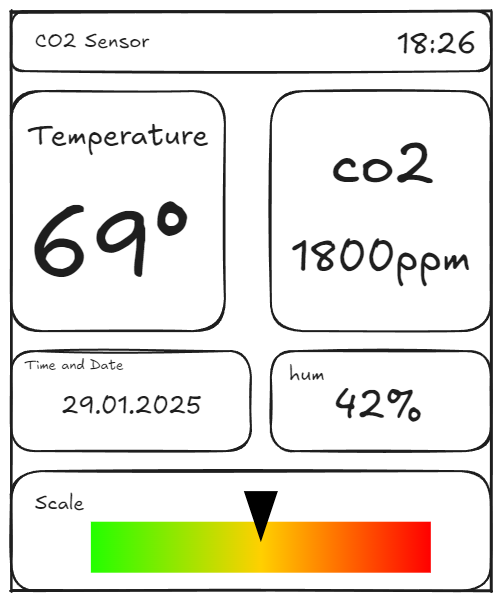
\includegraphics[width=0.35\textwidth]{files/Tobias/pics/Skizzen/Screen1_Sensor_Info.png}
\caption[Display Interface Skizze (Seite 1)]{}
\label{fig:display_skizze_seite_1}
\end{figure}

Am oberen Rand befindet sich die Seitenbezeichnung („CO2-Sensor“) sowie die aktuelle Uhrzeit in einem schmalen Feld. Darunter werden die Messwerte CO2 und Temperatur in größeren Feldern angezeigt, während sich das aktuelle Datum und die Luftfeuchtigkeit in kleineren Feldern darunter befinden. Ganz unten zeigt eine Skala die Luftqualität anhand des gemessenen Gaswiderstands an. Die Skala verläuft von Grün (gute Qualität) bis Rot (schlechte Qualität), und durch einen Zeiger wird der aktuelle Zustand markiert.

\begin{center}
    \textbf{Seite 2:}
\end{center}

\begin{figure}[!htb]
\centering
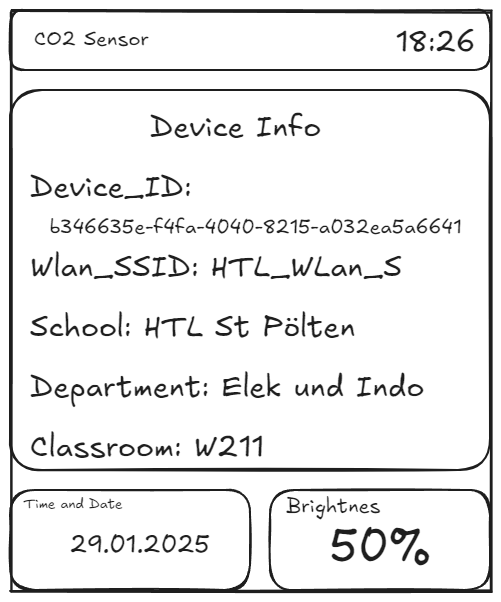
\includegraphics[width=0.35\textwidth]{files/Tobias/pics/Skizzen/Screen2_Info.png}
\caption[Display Interface Skizze (Seite 2)]{}
\label{fig:display_skizze_seite_2}
\end{figure}

Diese Seite der Benutzeroberfläche stellt Informationen über das Gerät bereit. Am oberen Rand befindet sich die Seitenbezeichnung sowie die aktuelle Uhrzeit. Direkt unter der Überschrift befindet sich eine große rechteckige Box mit der Überschrift „Device Info“. Innerhalb dieses Felds sind verschiedene Informationen aufgelistet:
\begin{itemize}
    \item Device ID
    \item WLAN-SSID
    \item School
    \item Department
    \item Classroom
\end{itemize}

Am unteren Ende der Seite befinden sich zwei Felder mit dem aktuellen Datum und der Helligkeitsstufe des Displays in Prozent.

\begin{center}
    \textbf{Seite 3:}
\end{center}

\begin{figure}[!htb]
\centering
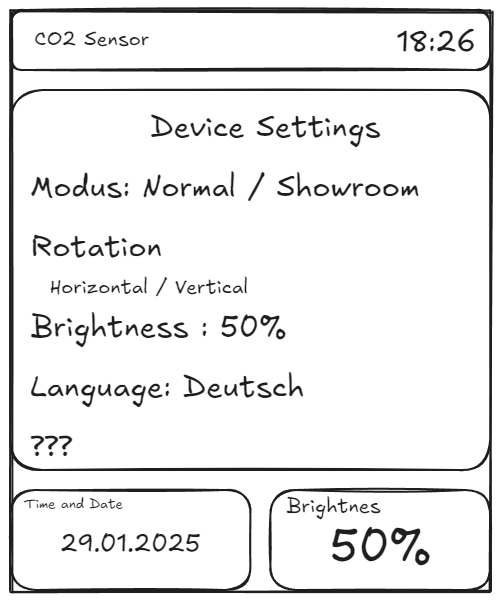
\includegraphics[width=0.35\textwidth]{files/Tobias/pics/Skizzen/Screen3_Settings.png}
\caption[Display Interface Skizze (Seite 3)]{}
\label{fig:display_skizze_seite_3}
\end{figure}

Die dritte Seite zeigt die Konfiguration des Geräts. Der Aufbau ähnelt den anderen Seiten: oben die Seitenbezeichnung und Uhrzeit, darunter eine große Box mit den Hauptinhalten. Hier können verschiedene Einstellungen vorgenommen werden:

\begin{itemize}
    \item Modus („Normal“ oder „Showroom“)
    \item Display-Ausrichtung (horizontal oder vertikal)
    \item Helligkeit
\end{itemize}

Zusätzliche Markierungen („???“) deuten an, dass noch weitere Einstellungsoptionen ergänzt werden können.

\begin{center}
    \textbf{Showroom:}
\end{center}

\begin{figure}[!htb]
\centering
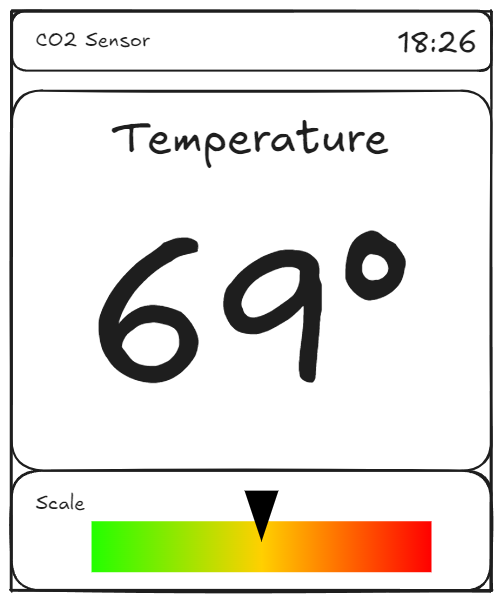
\includegraphics[width=0.35\textwidth]{files/Tobias/pics/Skizzen/Showroom1.png}
\caption[Display Interface Skizze (Showroom)]{}
\label{fig:display_skizze_showroom1}
\end{figure}

Der oben erwähnte Showroom ist ein Modus, in dem nicht eine fixe Seite angezeigt wird, sondern zwischen verschiedenen Seiten gewechselt wird. Der Sinn dahinter ist, die gemessenen Parameter einzeln und groß auf der Seite darzustellen. Dabei wird automatisch zwischen den Parametern gewechselt. Das obere Feld mit der Seitenbezeichnung und Uhrzeit sowie das untere Feld mit der Skala bleiben erhalten.

\end{inhalt} 
\begin{inhalt}
\chapter{Design \& Konzept}
\renewcommand*\chapterpagestyle{scrheadings}
\section{Software}

\subsection{Frontend}
Der Großteil des Frontends wird zunächst in Obsidian mithilfe des Excalidraw-Plugins entworfen, um zu veranschaulichen, wie eine Seite aussehen könnte.

\subsubsection{Dashboard}

Im Rahmen dieser Diplomarbeit wurde das Dashboard unter Berücksichtigung moderner Designansätze entwickelt. Es orientiert sich an dem Beispiel auf der Shadcn-Website (\url{https://ui.shadcn.com/examples/dashboard}), wobei die Gestaltung den spezifischen Anforderungen unseres Projekts angepasst wurde.

\begin{figure}[!htb] 
\centering 
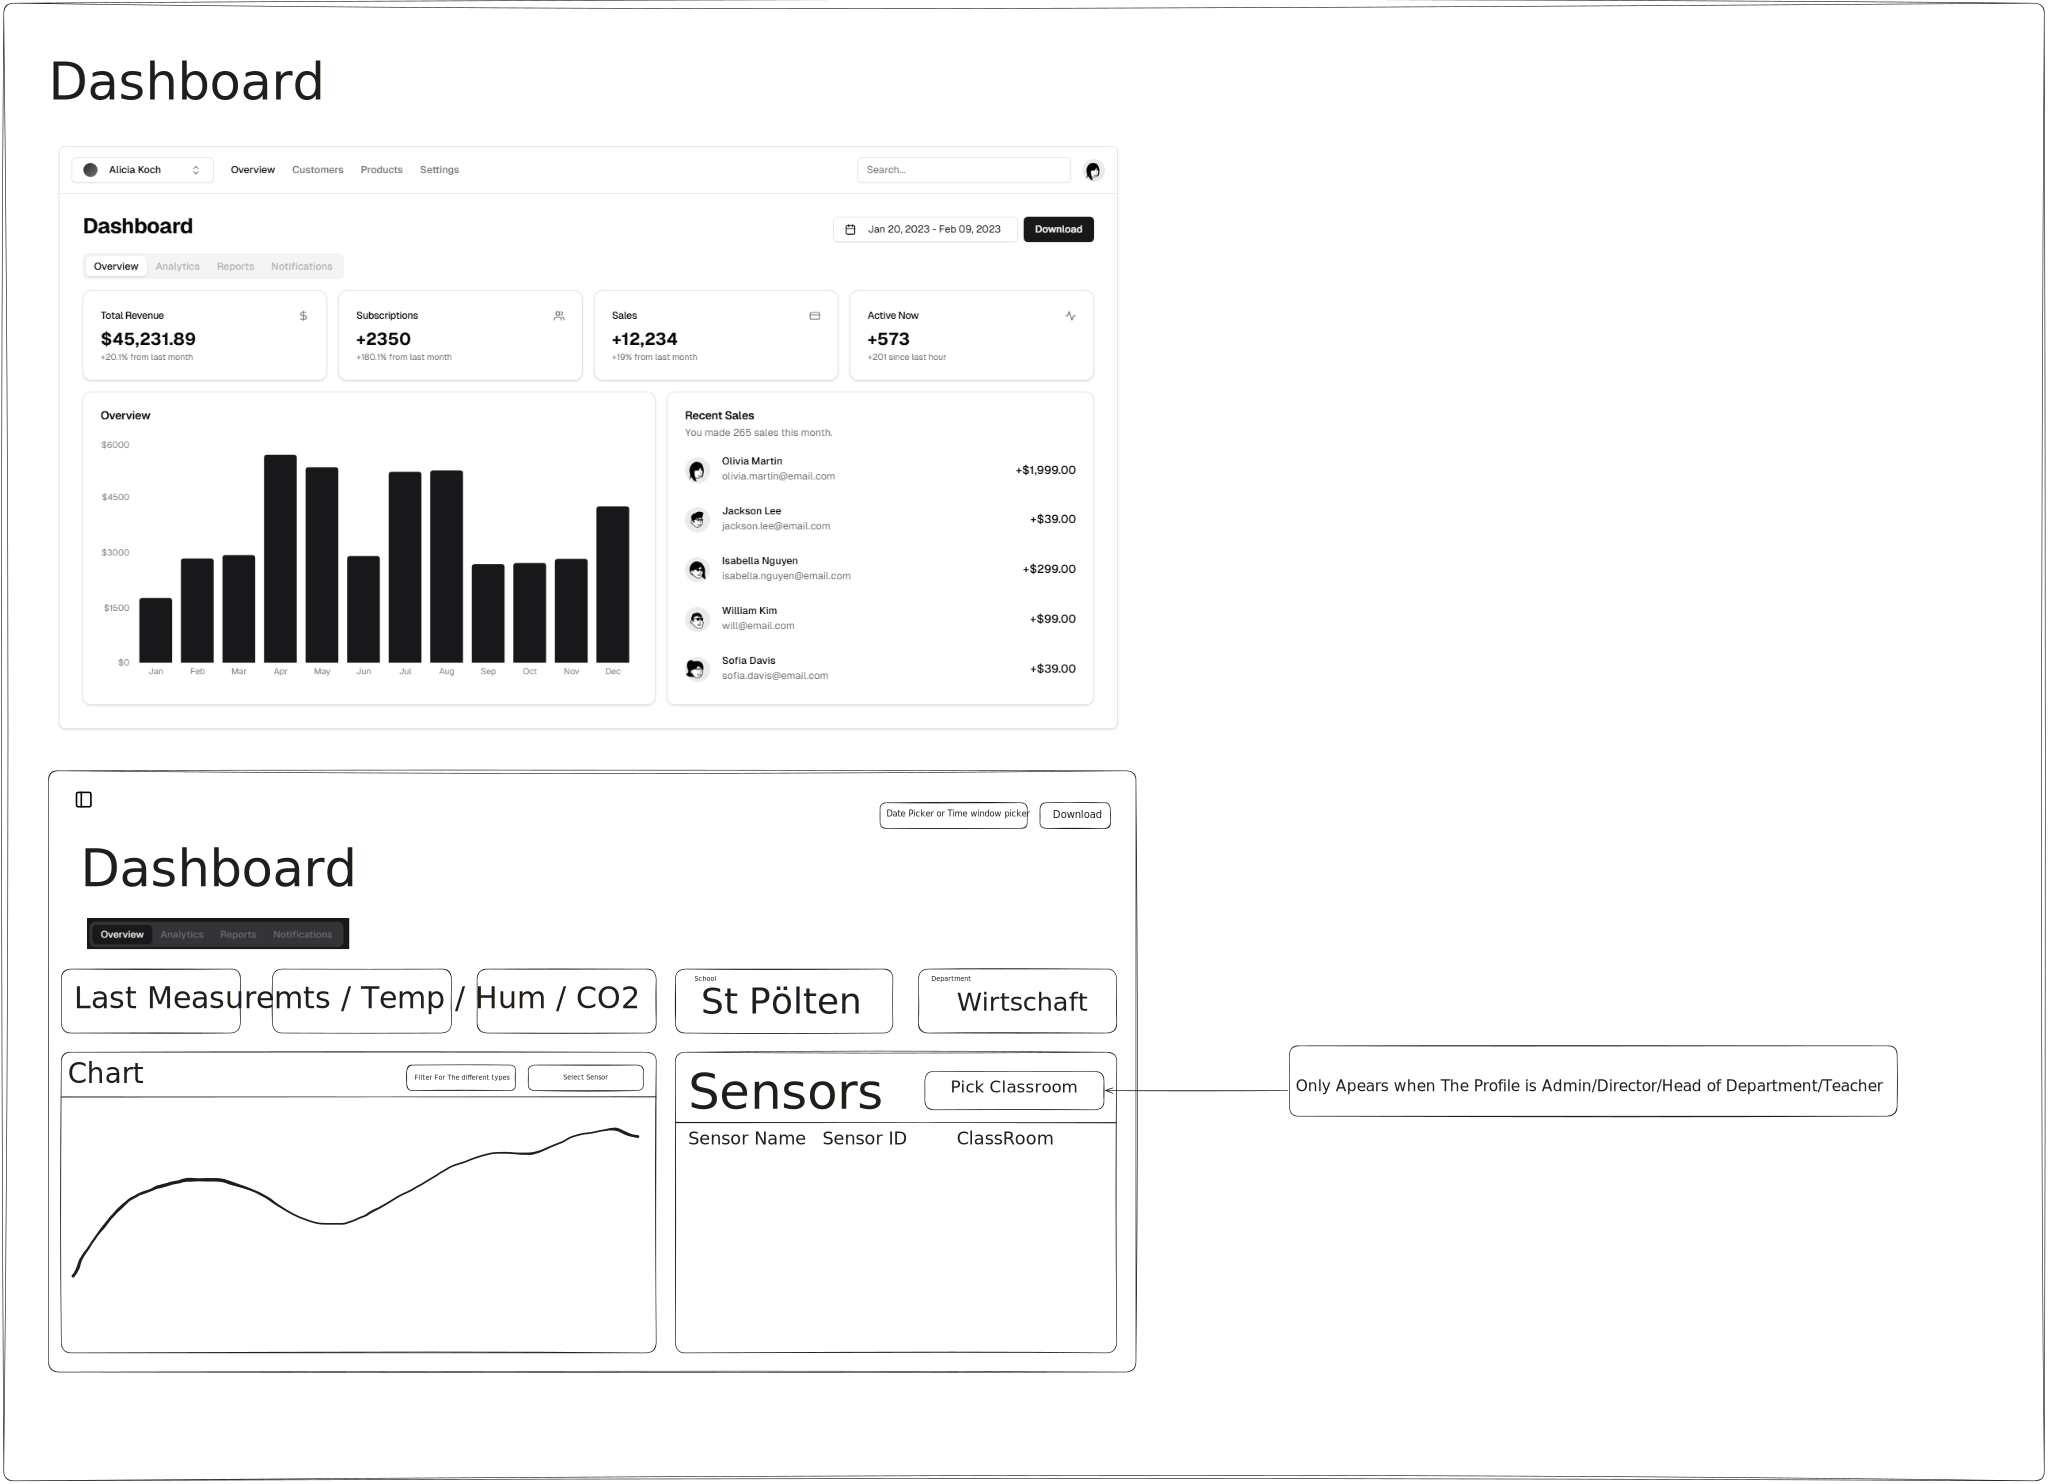
\includegraphics[width=1\textwidth]{files/Thomas/pics/Dashboard.excalidraw.png} 
\caption[Bildbezeichnung für Abbildungsverzeichnis]{Shadcn Example Dashboard} 
\label{fig:gehaeuse_internet_bild} 
\end{figure}

\subsubsection{Administrationsseiten}
\label{ref:Administrationsseiten}

Für die Entwicklung der Administrationsseiten wurde ein Konzept erarbeitet, das eine strukturierte und benutzerfreundliche Verwaltung der unterschiedlichen Datensätze ermöglicht. Auf der rechten Seite wird eine Tabelle angezeigt, in der alle relevanten Einträge übersichtlich dargestellt werden. Auf der linken Seite befindet sich eine Komponente zur Erstellung neuer Datensätze, welche die jeweiligen Tabellen ergänzt. Das System umfasst dabei separate Tabellen für Schulen, Abteilungen, Klassen, Sensoren und Benutzer, um eine differenzierte und effiziente Datenverwaltung zu gewährleisten. Zusätzlich erfolgt auf der Schul-Administrationsseite eine Visualisierung der Schulstandorte mittels einer Kartenansicht, um die räumliche Verteilung der Schulen anschaulich darzustellen.

\begin{figure}[!htb] 
\centering 
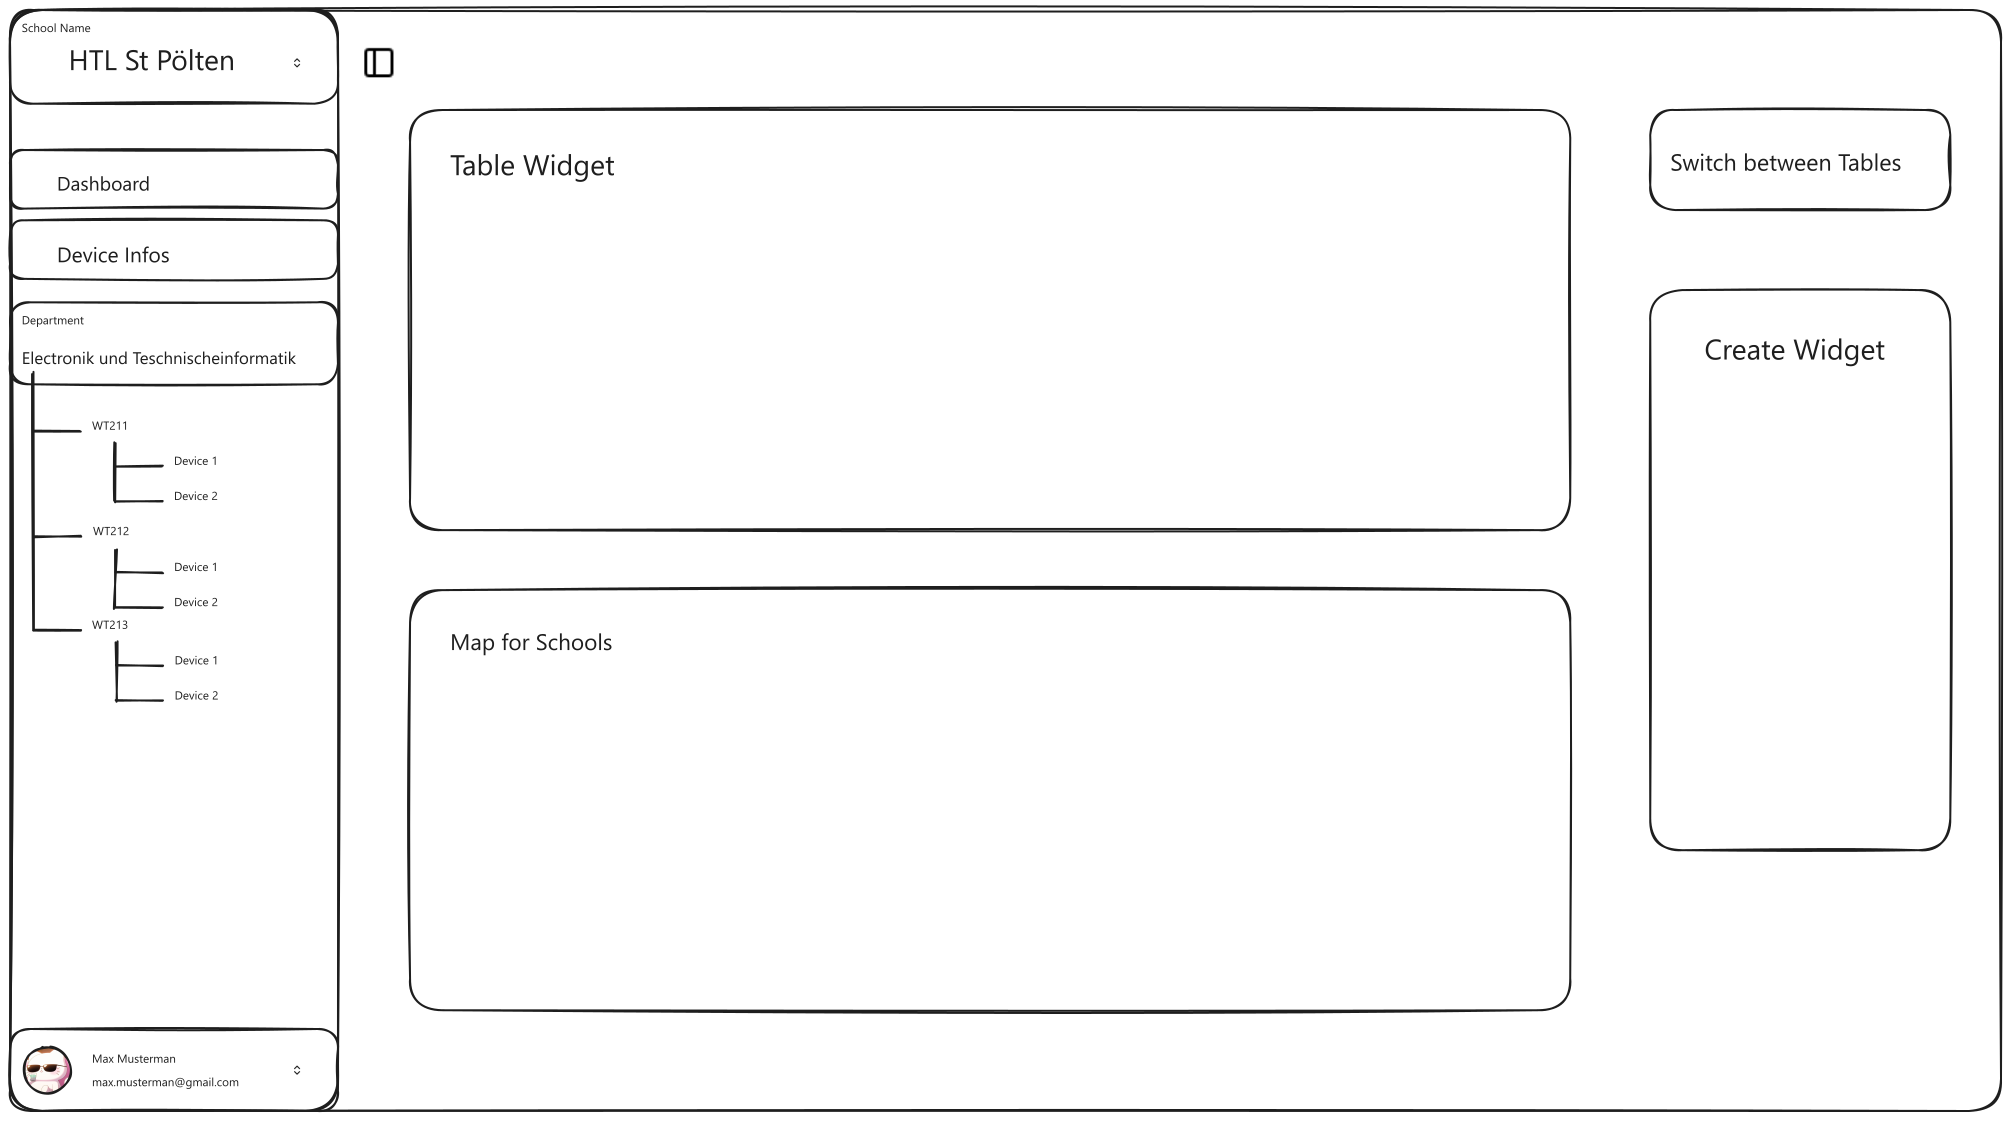
\includegraphics[width=1\textwidth]{files/Thomas/pics/Admin-Table.excalidraw.png} 
\caption[Bildbezeichnung für Abbildungsverzeichnis]{Beispiel einer Admin-Tabelle} 
\label{fig:gehaeuse_internet_bild} 
\end{figure}

\subsubsection{Seitenleiste}

\subsubsection{Seitenleiste}

Die Seitenleiste wurde aufgrund ihrer optimalen Form ausgewählt, um den Benutzeraccount übersichtlich darzustellen. Zudem ermöglicht sie es Administratoren, den aktuell ausgewählten Schulstandort zu wechseln, wodurch eine bessere Übersicht über die laufenden Prozesse erzielt wird. Unterhalb dieses Bereichs werden sämtliche Abteilungen mitsamt den zugehörigen Klassen und Sensoren angezeigt. Die Sichtbarkeit einzelner Abteilungen richtet sich nach der jeweiligen Benutzerrolle: Während Administratoren sowie Schulleiter (Direktoren) alle Abteilungen mit den entsprechenden Klassen und Geräten einsehen können, erhalten Lehrkräfte ausschließlich Zugriff auf die Abteilung, in der sie tätig sind, und Schülerinnen sowie Schüler sehen lediglich ihre eigene Klasse. 

Wird ein Sensor ausgewählt, gelangt der Benutzer auf das zugehörige Dashboard, welches detaillierte Informationen zu dem jeweiligen Sensor, der Klasse oder der Abteilung bereitstellt. Im unteren Bereich der Seitenleiste befindet sich zudem das Profilbild, ergänzt durch den Benutzernamen und die E-Mail-Adresse. Beim Anklicken dieses Elements öffnet sich eine Auswahlliste mit weiteren Optionen. Diese umfasst zum einen die Möglichkeit, über eine dedizierte Account-Seite den Account zu verwalten – beispielsweise den Namen, das Profilbild und den Benutzernamen zu ändern – zum anderen den Zugriff auf die in Abschnitt \ref{ref:Administrationsseiten} erläuterten Administrationsseiten sowie eine Einstellungsseite. Auf dieser können unter anderem persönliche Schlüssel für das zugeordnete Gerät sowie weitere Funktionen eingesehen werden. Abschließend steht ein Logout-Button zur Verfügung, der den Benutzer aus dem System abmeldet und zur Login-Seite zurückführt.

\begin{figure}[!htb] 
\centering 
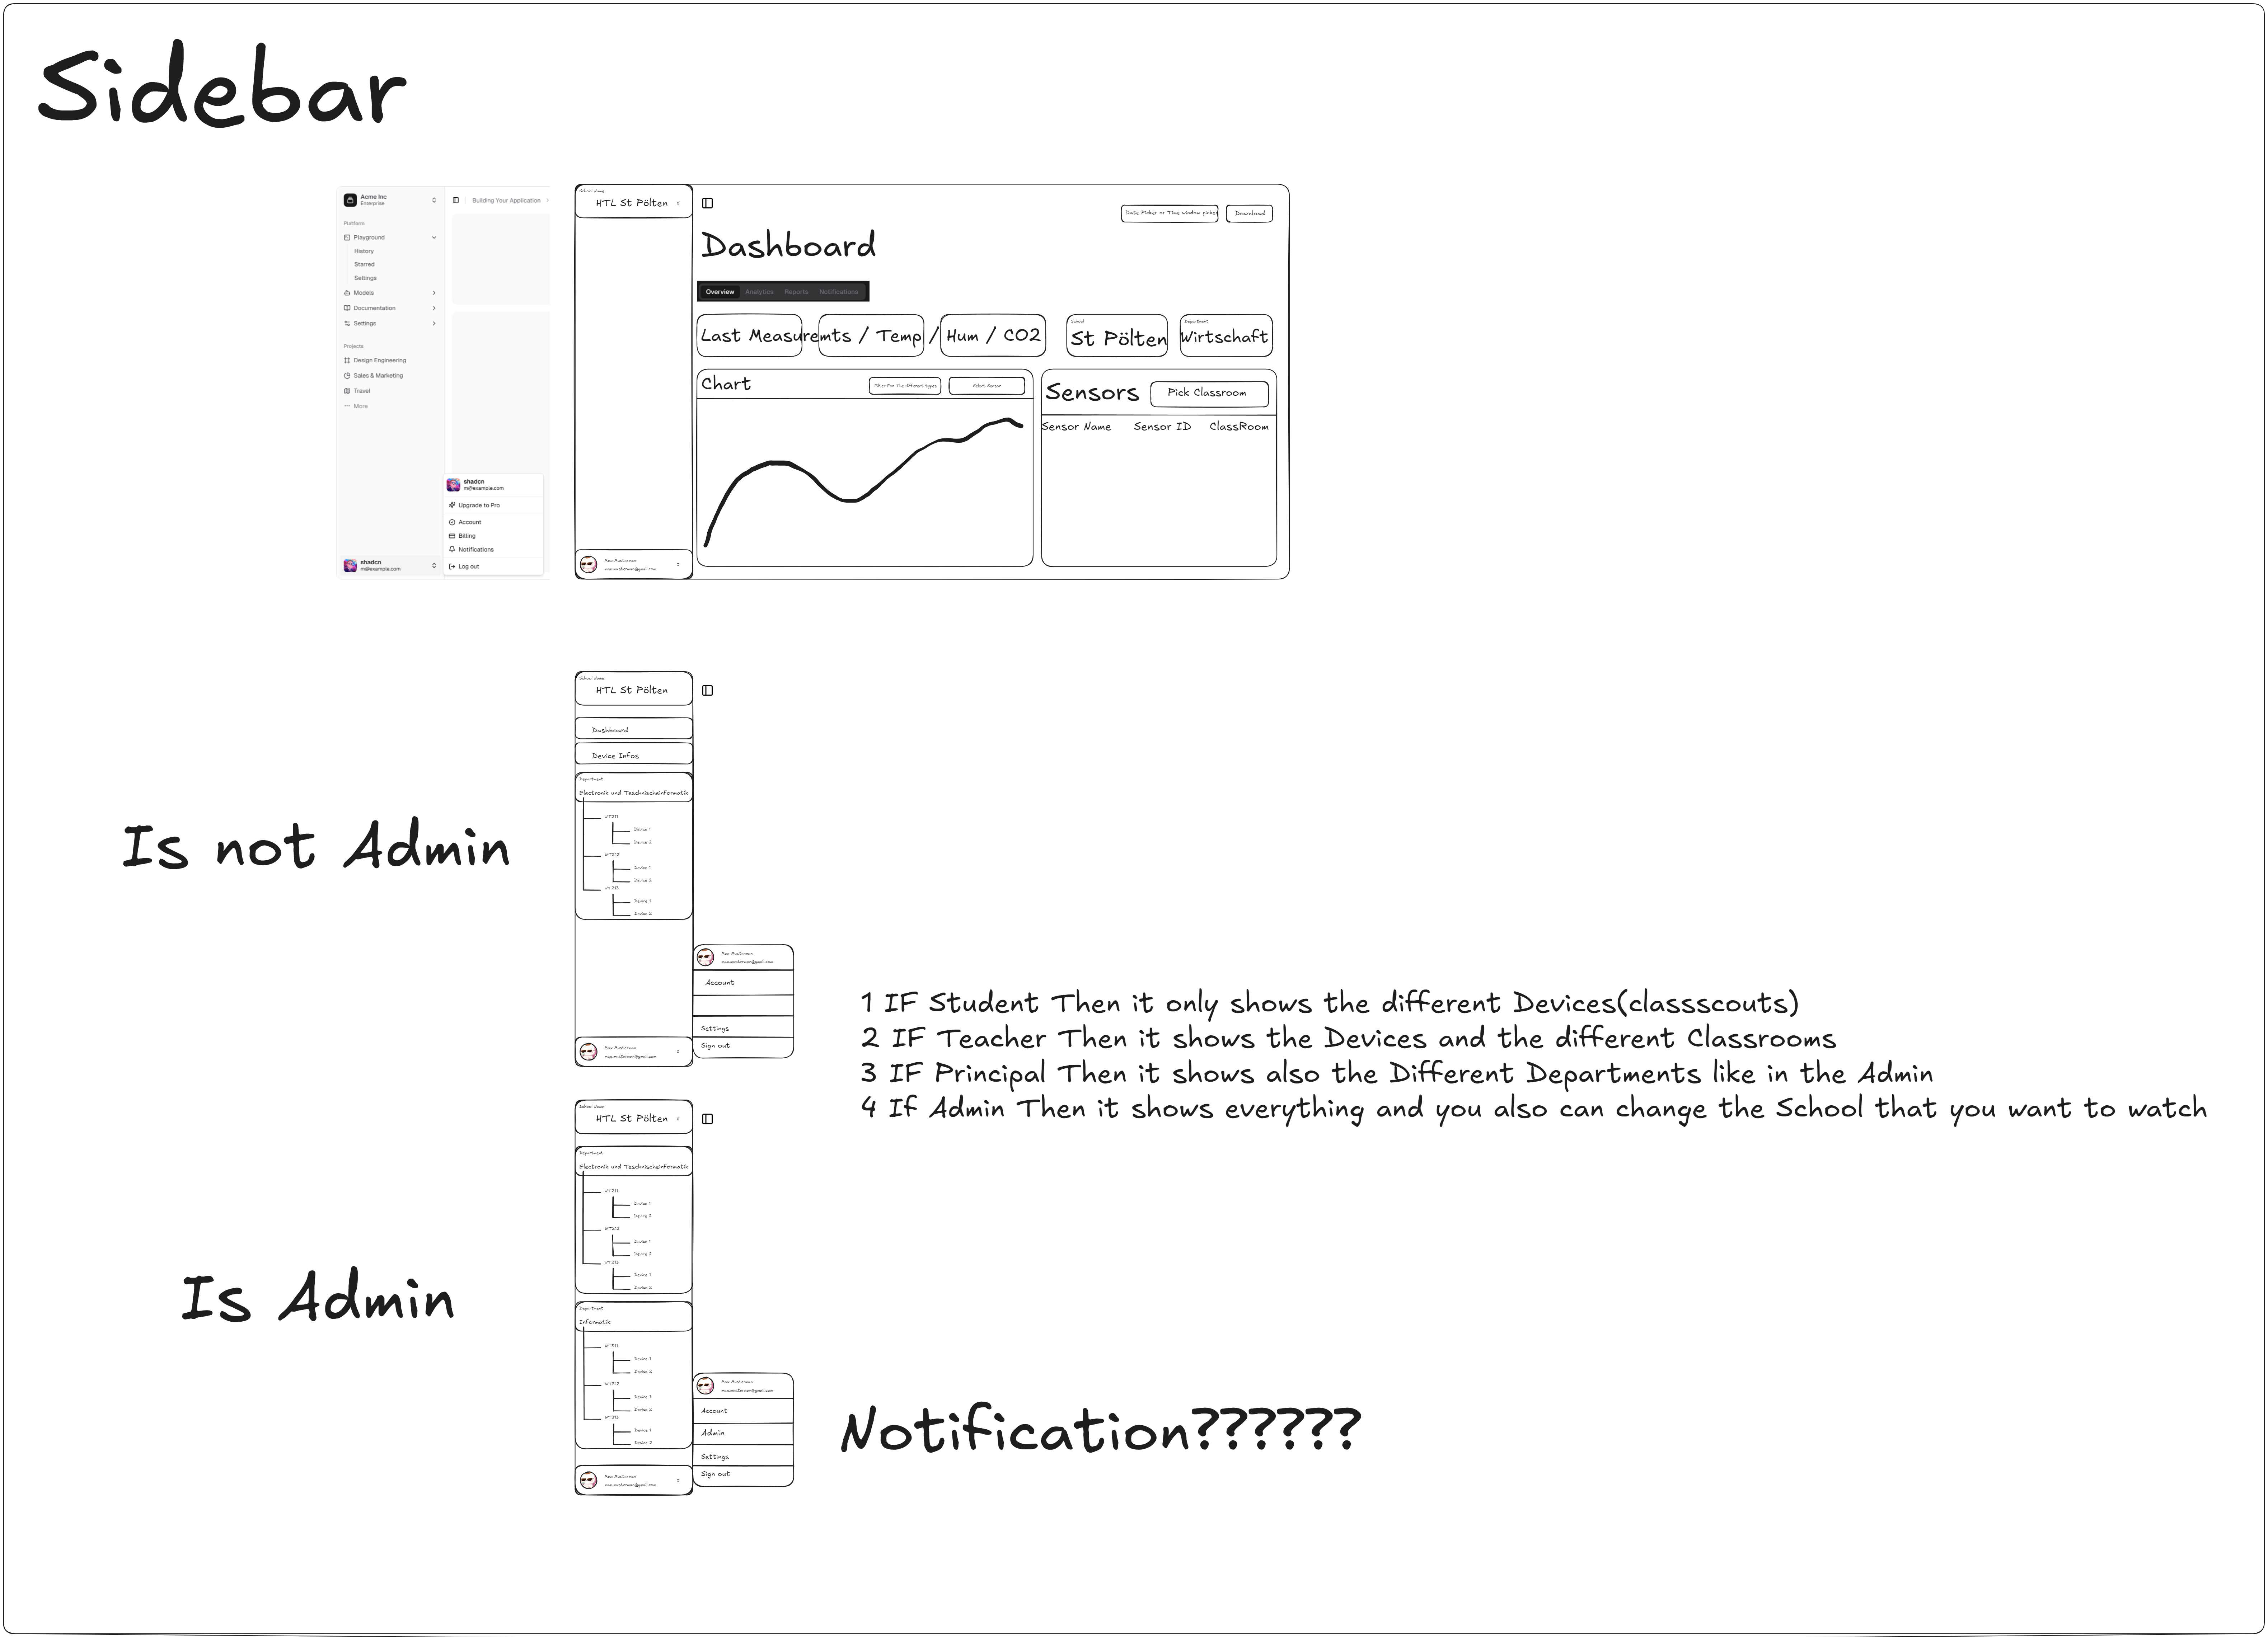
\includegraphics[width=1\textwidth]{files/Thomas/pics/Sidebar.excalidraw.png} 
\caption[Bildbezeichnung für Abbildungsverzeichnis]{Beispiel der Seitenleiste} 
\label{fig:gehaeuse_internet_bild} 
\end{figure}

\subsection{Backend}

Im Folgenden wird das Design des Backends erläutert. Das System ist in der Lage, verschiedene Messwerte zu verarbeiten, darunter CO\textsubscript{2}-Konzentrationen, Feuchtigkeitswerte, Temperaturwerte, Gaswiderstandswerte sowie einen Zeitstempel. Diese Daten werden im JSON-Format vom Backend empfangen. Zur Sicherstellung einer einheitlichen Datenstruktur wurde das folgende JSON-Schema definiert:

\begin{lstlisting}[style=myjson]
{
    "measured_at": "2024-10-23T12:29:02.379+00:00",
    "co2": 6,
    "hum": 7,
    "temp": 8,
    "gasres": 9
}
\end{lstlisting}

Zur eindeutigen Identifizierung der einzelnen Sensoren wird beim Anlegen eines Sensors auf der Administrationsseite stets eine Sensor-ID generiert. Diese dient als einzigartiger Identifikator, der es ermöglicht, die Messdaten den entsprechenden Sensoren zuzuordnen. Dementsprechend wird die Sensor-ID in den JSON-Daten mitübertragen:

\begin{lstlisting}[style=myjson]
{
    "token": "d192f90b-a5b8-4767-b5af-59ec40fe03c2",
    "measured_at": "2024-10-23T12:29:02.379+00:00",
    "co2": 6,
    "hum": 7,
    "temp": 8,
    "gasres": 9
}
\end{lstlisting}

Ein Problem tritt auf, wenn mehrere Messdaten gleichzeitig versendet werden sollen, da mehr Messpunkte erfasst werden, als in einer einzelnen Übertragung enthalten sein können. Zur Lösung dieses Problems wurde ein erweitertes JSON-Format entwickelt, das die Übermittlung mehrerer Messdatensätze in einer einzigen Nachricht ermöglicht:

\begin{lstlisting}[style=myjson]
{
    "token": "d192f90b-a5b8-4767-b5af-59ec40fe03c2",
    "data": [
        {
            "measured_at": "2024-10-23T12:28:02.379+00:00",
            "co2": 3,
            "hum": 4,
            "temp": 5,
            "gasres": 6
        },
        {
            "measured_at": "2024-10-23T12:29:02.379+00:00",
            "co2": 6,
            "hum": 7,
            "temp": 8,
            "gasres": 9
        },
        {
            "measured_at": "2024-10-23T12:30:02.379+00:00",
            "co2": 9,
            "hum": 10,
            "temp": 11,
            "gasres": 12
        }
    ]
}
\end{lstlisting}

Mit diesem erweiterten Datenformat ist das Backend in der Lage, die empfangenen Messdaten effizient in der Datenbank zu speichern.

\section{Datenbank}

Bei der Planung der Datenbankstruktur wurde zunächst festgestellt, dass Supabase zwar über die integrierte Authentifizierungstabelle theoretisch benutzerspezifische Daten abspeichern könnte, dies jedoch nicht vorgesehen ist. Aus diesem Grund wurde entschieden, eine eigene Tabelle für Benutzer anzulegen.

Im nächsten Schritt musste eine sinnvolle Struktur für die Verwaltung der Sensoren entworfen werden. Da das System nicht ausschließlich für die HTL St. Pölten vorgesehen ist, sondern auch von anderen Bildungseinrichtungen genutzt werden könnte, wurde die Datenbank entsprechend erweitert. Es wurde eine Tabelle \textit{Schools} erstellt, um mehrere Schulen abbilden zu können.

Da eine Schule in verschiedene Abteilungen untergliedert ist, wurden zusätzlich die Tabellen \textit{Departments} (Abteilungen) sowie \textit{Classes} (Klassen) angelegt. Diese Struktur ermöglicht eine klare Zuordnung und Verwaltung der Sensoren auf Klassen- bzw. Abteilungsebene innerhalb der jeweiligen Schule.

Für die eigentlichen Sensordaten wurden zwei weitere Tabellen erstellt: \textit{Sensors} und \textit{Sensor-Readings}. Die Trennung dieser Informationen ist notwendig, da bei einer Speicherung der Messwerte direkt in der \textit{Sensors}-Tabelle lediglich die aktuellen Werte abrufbar wären. Da jedoch geplant ist, die historischen Messwerte in Form von Zeitdiagrammen darzustellen, müssen diese dauerhaft gespeichert werden. Aus diesem Grund enthält die Tabelle \textit{Sensor-Readings} zeitlich zuordenbare Einzelmessungen, welche sich eindeutig einem Sensor zuordnen lassen.


\newpage


\begin{sidewaysfigure}[!htb]
  \centering
  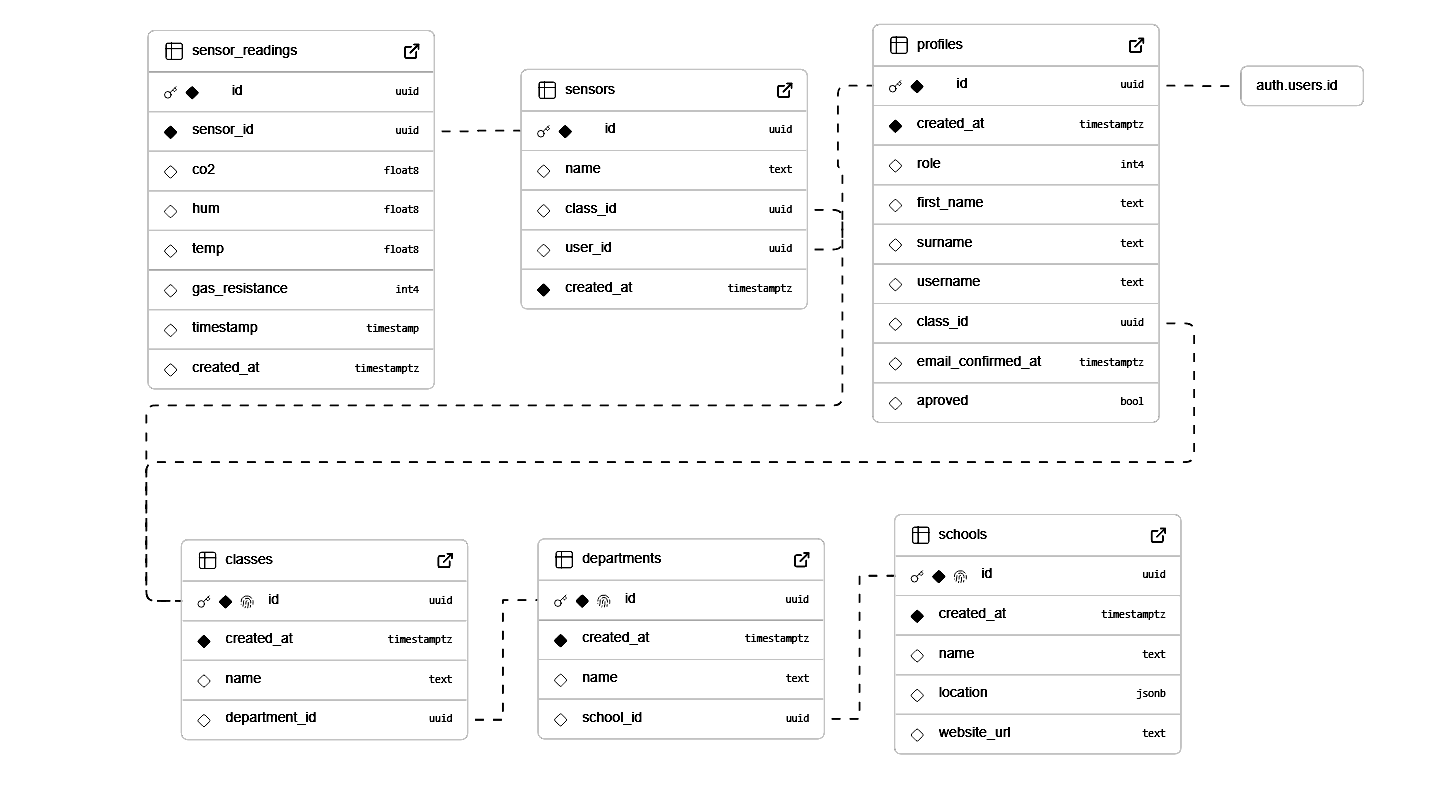
\includegraphics[scale=0.45]{files/Thomas/pics/output.png}
  \caption[Bildbezeichnung für Abbildungsverzeichnis]{Your caption text here.}
  \label{fig:gehaeuse_internet_bild}
\end{sidewaysfigure}

\clearpage  % <-- Forces LaTeX to place the figure here


\newpage

\section{Gehäuse}

Im Zuge der Gehäuseentwicklung wurde eine umfassende Internetrecherche durchgeführt. Dabei stießen wir auf eine Abbildung (vgl. Abb. \ref{fig:gehaeuse_internet_bild}), die als Inspiration für die weitere Gestaltung diente. Basierend auf diesem Vorbild wurde ein eigenes Gehäusemodell entworfen und optimal an die Anforderungen unseres Geräts angepasst.


\begin{figure}[!htb]
\centering
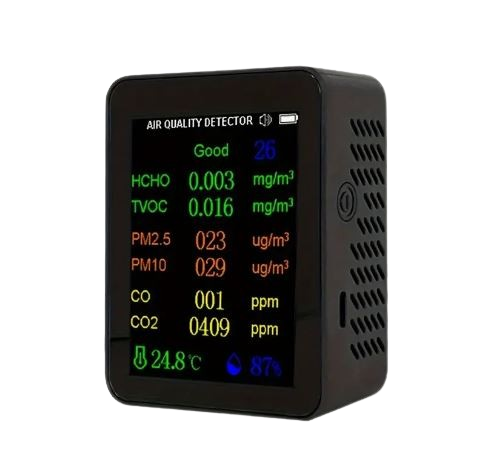
\includegraphics[width=0.75\textwidth]{files/Thomas/pics/new/Temu-removebg-preview.png}
\caption[Bildbezeichnung für Abbildungsverzeichnis]{}
\label{fig:gehaeuse_internet_bild}
\end{figure}

Da man aber irgendwie das gane nicht ganz drucken kann und die pcb auch reingegeben werden muss wurde sich auf ein Zweiteiliges Gehäuse entschieden das Durch dieses Youtube Video(https://www.youtube.com/watch?v=E0NVC8xhf3I&t) wurde dann die Idee entnommen das man doch mit Clips Arbeiten konnte 



\end{inhalt}   
%Methoden(LaTeX File) einfügen


%Chapter 5 Hardwareentwicklung
\responsible{Tobias Geppl} 
\begin{inhalt}
\renewcommand*\chapterpagestyle{scrheadings}
\chapter{Hardwareentwicklung}

Einführung in Tobias Teil Kurze Erklärung
\section{Komponentenwahl}
\subsection{Sensoren}
\subsection{Mikrocontroller}
\subsection{Bedienelemente}





\section{Versorgungen \& Ansteuerungen}
\subsection{Bussysteme}
\subsection{Spannungsversorgungen}

\section{Pin-Layout \& Schematik}


\section{PCB-Design}


\end{inhalt}                                      

%Chapter 6 Mikrocontroller-Programmierung
\responsible{Tobias Geppl} 
\begin{inhalt}
\renewcommand*\chapterpagestyle{scrheadings}

\chapter{Mikrocontroller-Programmierung}

Die Programmierung des Raspberry Pi Pico W erfolgte mithilfe der Entwicklungsumgebung Visual Studio Code (Kap. \ref{sec:VS-Code}) in Kombination mit der Raspberry Pi Pico-Erweiterung (Kap. \ref{sec:PicoExtension}). Als Programmiersprache wurde C/C++ verwendet. Die Projektstruktur basierte auf dem CMake-Buildsystem mit der Verwendung des offiziellen Pico SDK (\ref{…}). 

\section{I2C:} \label{I2C_Programmierung}

Der Raspberry Pico W besitzt zwei I2C-instanzen: i2c0 und i2c1. Bei der Initialisierungsfunktion i2c\_init(), muss die I2C-Instanz sowie die Taktgeschwindigkeit übergeben werden. Diese Funktion wird von dem Pico SDK (\ref{….}) bereitgestellt. 

\begin{lstlisting} [style=mytsx]
i2c_init(i2c0, 100 * 1000); // i2c0 mit 100 kHz Takt initialisieren
\end{lstlisting}
\index{Code Snippet 1@\hyperref[code:snippet1]{Snippet 1}}


Anschließend werden die entsprechenden GPIO-Pins sowie die internen Pullup-Widerstände gesetzt, da sich keine physischen Pullup-Widerstände auf den Leitungen befinden. 

\\bigskip \\


\textbf{Schreiben:}

Um Daten auf den I2C-Bus zu schreiben, wird folgende Funktion benutzt:

\begin{lstlisting} [style=mytsx]
int i2c_write_blocking(i2c_inst_t *i2c, uint8_t addr, const uint8_t *src, size_t len, bool nostop);
\end{lstlisting}
\index{Code Snippet 1@\hyperref[code:snippet1]{Snippet 1}}

\begin{table}[H]
\centering
\renewcommand{\arraystretch}{1.3}
\begin{tabular}{|l|p{10cm}|}
\hline
\rowcolor{cyan!20}
\textbf{Parameter} & \textbf{Bedeutung} \\
\hline
\texttt{i2c} & I²C-Instanz (\texttt{i2c0} oder \texttt{i2c1}) \\
\hline
\texttt{addr} & I²C-Adresse des Slaves \\
\hline
\texttt{src} & Zeiger auf das zu sendende Datenarray \\
\hline
\texttt{len} & Anzahl der zu sendenden Bytes \\
\hline
\texttt{nostop} & \texttt{false} = STOP \newline
\texttt{true} = REPEATED START \\
\hline
\end{tabular}
\caption{I2C-Sende-Funktion Parameterübersicht}
\label{tab:i2c_parameter}
\end{table}




\textbf{Lesen:}

Um Daten vom I2C-Bus zu lesen, wird folgende Funktion benutzt:

\begin{lstlisting} [style=mytsx][caption={I2C Initialisierung}, label={code:i2c_init}]
int i2c_read_blocking(i2c_inst_t *i2c, uint8_t addr, uint8_t *dst, size_t len, bool nostop);
\end{lstlisting}
\index{Code Snippet 1@\hyperref[code:snippet1]{Snippet 1}}

\begin{table}[H]
\centering
\renewcommand{\arraystretch}{1.3}
\begin{tabular}{|l|p{10cm}|}
\hline
\rowcolor{cyan!20}
\textbf{Parameter} & \textbf{Bedeutung} \\
\hline
\texttt{i2c} & I2C-Instanz (\texttt{i2c0} oder \texttt{i2c1}) \\
\hline
\texttt{addr} & I2C-Adresse des Slaves \\
\hline
\texttt{dst} & Zielpuffer für empfangene Bytes \\
\hline
\texttt{len} & Anzahl der zu lesenden Bytes \\
\hline
\texttt{nostop} & Meist \texttt{false}, es sei denn, ein \texttt{REPEATED START} ist erforderlich \\
\hline
\end{tabular}
\caption{I2C-Lese-Funktion Parameterübersicht}
\label{tab:i2c_read_parameters}
\end{table}

Beim Lesen muss zuerst das entsprechende Register geschrieben werden, um anschließend die Daten daraus auszulesen. 

\bigskip \\
Die Lese- und Schreibfunktionen werden vom Pico SDK bereitgestellt.

\textbf{I2C-Beispiel:}

Als Beispiel wurde vom Host die Daten 0xAA an den Slave mit der Adresse 0x28 gesendet. 

\begin{lstlisting} [style=mytsx][caption={I2C Initialisierung}, label={code:i2c_init}]
test_buffer[0] = 0xAA;
i2c_write_blocking(i2c, 0x28, test_buffer, 1, false);
\end{lstlisting}
\index{Code Snippet 1@\hyperref[code:snippet1]{Snippet 1}}

\begin{figure}[!htb]
\centering
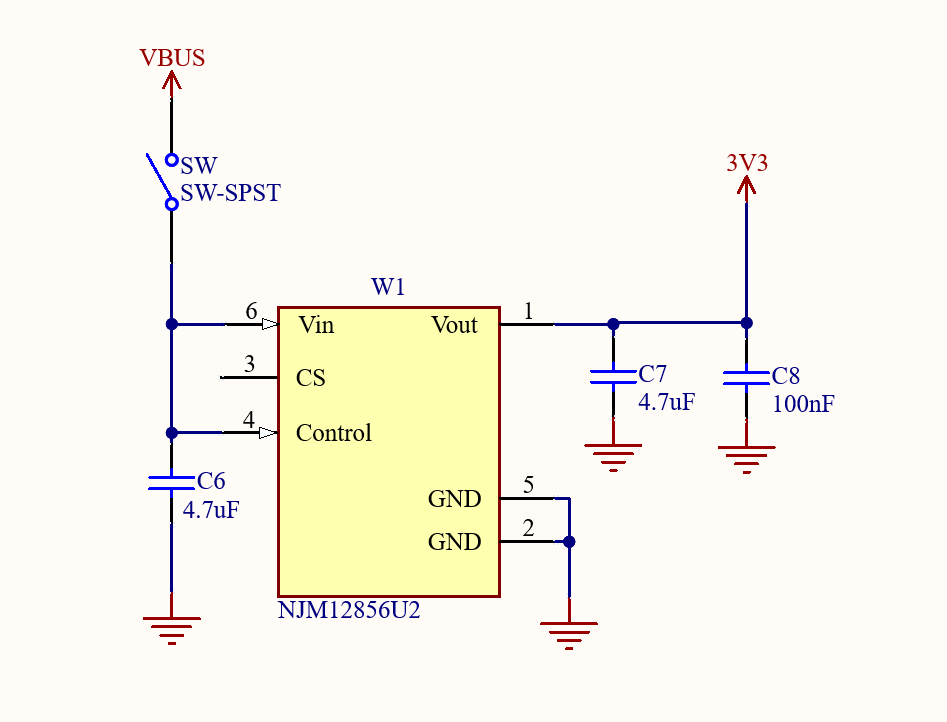
\includegraphics[width=0.75\textwidth]{files/Tobias/pics/Schaltungen/Schematik/3V3_Converter_Schematik.PNG}
\caption[3,3V Spannungsregler Schematik]{3,3V Spannungsregler Schematik}
\label{fig:3,3V Spannungsregler Schematik}
\end{figure}



\section{PAS CO2}

Da für den PAS CO2-Sensor keine Bibliotheken speziell für den Raspberry Pi Pico W verfügbar sind, wurde mithilfe des Datenblatts \cite{Raspberry_Pi_Pico_W} sowie des Programming-Guides \cite{PASCO2_ProgrammingGuide} des PAS CO2 eine eigene Bibliothek geschrieben.

\bigskip \\

\textbf{Sensor Struktur:}

Der Sensor wird im Programmcode als folgende Struktur aufgebaut:

\begin{lstlisting} [style=mytsx][caption={I2C Initialisierung}, label={code:i2c_init}]
typedef struct {
    uint8_t i2c_address;
    i2c_inst_t* i2c;
    uint8_t lsb;
    uint8_t msb;
    uint8_t data_rdy;
    uint16_t result;
} Pas_co2;
\end{lstlisting}
\index{Code Snippet 1@\hyperref[code:snippet1]{Snippet 1}}

\begin{table}[H]
\centering
\renewcommand{\arraystretch}{1.3}
\begin{tabular}{|l|p{11cm}|}
\hline
\rowcolor{cyan!20}
\textbf{Variable} & \textbf{Beschreibung} \\
\hline
\texttt{i2c\_address} & I2C-Adresse des Sensors\\
\hline
\texttt{i2c} & Zeiger auf die verwendete I²C-Instanz \\
\hline
\texttt{lsb} & Low-Byte der CO2-Messung (Least Significant Byte) \\
\hline
\texttt{msb} & High-Byte der CO2-Messung (Most Significant Byte) \\
\hline
\texttt{data\_rdy} & Statusspeicher – zeigt an, ob neue Daten vorhanden sind \\
\hline
\texttt{result} & Letzter berechneter CO2-Wert in ppm, zusammengesetzt aus \texttt{msb} und \texttt{lsb} \\
\hline
\end{tabular}
\caption{Sensorstruktur PASCO2 - Variablenübersicht}
\label{tab:co2_struct_vars}
\end{table}

\textbf{Initialisierung:}

Der PASCO2 besitzt drei verschiedene Betriebsmodi: Idle Mode, Continuous Mode und Single-Shot Mode, die über das MEAS\_CFG-Register eingestellt werden. In diesem Fall wird der Continuous Mode gewählt. In diesem Modus wird periodisch eine CO2-Messung ausgelöst. Sobald eine Messung abgeschlossen ist, wechselt der Sensor automatisch in den Idle-Mode (Ruhemodus) und wacht selbstständig zur nächsten Messung wieder auf. Die Periode der Messungen lässt sich mit den Registern MEAS\_RATE\_H und MEAS\_RATE\_L im Bereich von 5 bis 4095 Sekunden einstellen. In diesem Fall wird ein 10 Sekunden Intervall gewählt.

\begin{lstlisting} [style=mytsx][caption={I2C Initialisierung}, label={code:i2c_init}]

    uint8_t buffer[2];

    // Setzt die Messrate auf 1 Hz
    buffer[0] = MEAS_RATE_H;
    buffer[1] = 0x00;
    i2c_write_blocking(sensor->i2c, sensor->i2c_address, buffer, 2, false);
    
    buffer[0] = MEAS_RATE_L;
    buffer[1] = 0x01;
    i2c_write_blocking(sensor->i2c, sensor->i2c_address, buffer, 2, false);

    // Setzt den Sensor in den Continuous-Modus
    buffer[0] = MEAS_CFG;
    buffer[1] = 0x02;
    i2c_write_blocking(sensor->i2c, sensor->i2c_address, buffer, 2, false);
}
\end{lstlisting}


\textbf{CO2-Messung:}

In der Funktion pas\_co2\_read(Pas\_co2* sensor) wird die CO2-Konzentration ausgelesen. Dazu wird zunächst das MEAS\_STS-Register abgefragt, um zu prüfen, ob neue Daten vorhanden sind. Ist dies der Fall, wird die CO2-Konzentration aus zwei Registern, CO2PPM\_H und CO2PPM\_L, ausgelesen. Anschließend werden die beiden Register miteinander kombiniert und das Ergebnis gespeichert.

\begin{lstlisting} [style=mytsx][caption={I2C Initialisierung}, label={code:i2c_init}]
        // CO2 PPM High-Byte lesen
        reg = CO2PPM_H;
        i2c_write_blocking(sensor->i2c, sensor->i2c_address, &reg, 1, true);
        i2c_read_blocking(sensor->i2c, sensor->i2c_address, &sensor->msb, 1, false);

        // CO2 PPM Low-Byte lesen
        reg = CO2PPM_L;
        i2c_write_blocking(sensor->i2c, sensor->i2c_address, &reg, 1, true);
        i2c_read_blocking(sensor->i2c, sensor->i2c_address, &sensor->lsb, 1, false);

        // High- und Low-Byte kombinieren und speichern
        sensor->result = (sensor->msb << 8) | sensor->lsb;
\end{lstlisting}


\textbf{Ergebnisabruf:}

Die Funktion pas\_co2\_get\_result(const Pas\_co2* sensor) greift auf das gespeicherte Ergebnis zu und gibt es zurück. 

\begin{lstlisting} [style=mytsx][caption={I2C Initialisierung}, label={code:i2c_init}]
uint16_t pas_co2_get_result(const Pas_co2* sensor) {
    return sensor->result;
}
\end{lstlisting}

\section{BME688}

Für den BME688 wurde eine Bibliothek geschrieben, die auf der BME68x-C-Bibliothek von Bosch basiert. Die eigentliche Kommunikation mit dem Sensor erfolgt über eigene Funktionen, während die Bosch-Bibliothek die Konfiguration und Datenverarbeitung übernimmt.

\textbf{Sensor Struktur}
\begin{lstlisting} [style=mytsx][caption={I2C Initialisierung}, label={code:i2c_init}]

typedef struct {
    i2c_inst_t *i2c;
    uint8_t address;
    struct bme68x_dev dev;
    struct bme68x_conf conf;
    struct bme68x_heatr_conf heatr_conf;
} BME688;
\end{lstlisting}

\begin{table}[H]
\centering
\renewcommand{\arraystretch}{1.3}
\begin{tabular}{|l|p{11cm}|}
\hline
\rowcolor{cyan!20}
\textbf{Feld} & \textbf{Bedeutung} \\
\hline
\texttt{i2c} & I²C-Instanz (\texttt{i2c0} oder \texttt{i2c1}) \\
\hline
\texttt{address} & I²C-Adresse des Sensors \\
\hline
\texttt{dev} & Kern-Datenstruktur der Bosch-Bibliothek \\
\hline
\texttt{conf} & Konfiguration der Sensor-Messparameter \\
\hline
\texttt{heatr\_conf} & Konfiguration der Heizung \\
\hline
\end{tabular}
\caption{Sensorstruktur BME688 - Variablenübersicht}
\label{tab:bme688_struct}
\end{table}


\bigskip \\
\textbf{Initialisierung:}

\begin{lstlisting} [style=mytsx][caption={I2C Initialisierung}, label={code:i2c_init}]
bool bme688_init(BME688 *sensor, i2c_inst_t *i2c, uint8_t address, uint8_t sda, uint8_t scl);
\end{lstlisting}

Die Initialisierungsfunktion weist die I2C-Instanz sowie die Adresse des Sensors zu. Sie setzt ebenfalls Funktionszeiger auf die Adapterfunktionen. 

\bigskip \\
\textbf{Sensorstart:}

\begin{lstlisting} [style=mytsx][caption={I2C Initialisierung}, label={code:i2c_init}]
bool bme688_begin(BME688 *sensor);
\end{lstlisting}

Die Startfunktion initialisiert den Bosch-Treiber, setzt Oversampling und Heizkonfigurationen, sowie den Forced-Modus des Sensors. 

\bigskip \\
\textbf{Daten lesen:}

\begin{lstlisting} [style=mytsx][caption={I2C Initialisierung}, label={code:i2c_init}]
bool bme688_read_data(BME688 *sensor, float *temperature, float *humidity, float *pressure, float *gas_resistance);
\end{lstlisting}

Diese Funktion startet eine Messung im Forced-Modus und wartet die notwendige Heiz,- und Messdauer des Sensors ab. Temperatur, Luftfeuchtigkeit, Druck und Gaswiderstand werden ausgelesen. 

\bigskip \\
\textbf{Adapterfunktionen:}

Folgende Funktionen dienen als I2C-Adapterfunktionen zwischen der Bosch-Bibliothek und der I2C-Kommunikation mit dem Sensor:

\begin{lstlisting} [style=mytsx][caption={I2C Initialisierung}, label={code:i2c_init}]
static int8_t bme688_i2c_read(uint8_t reg, uint8_t *data, uint32_t len, void *intf);
\end{lstlisting}

\begin{lstlisting} [style=mytsx][caption={I2C Initialisierung}, label={code:i2c_init}]
static int8_t bme688_i2c_write(uint8_t reg, const uint8_t *data, uint32_t len, void *intf);
\end{lstlisting}

\begin{lstlisting} [style=mytsx][caption={I2C Initialisierung}, label={code:i2c_init}]
static void bme688_delay_us(uint32_t period, void *intf);
\end{lstlisting}

Diese Funktionen werden als Callback an die Bosch-Bibliothek übergeben. Sie nutzen die Funktionen i2c\_write\_blocking() und i2c\_read\_blocking() (Kap. \ref{I2C_Programmierung}) aus dem Pico SDK.


\section{Display Ansteuerung}

Für die Ansteuerung des 2-Zoll LCD-Displays von Waveshare wird die Open-Source-Grafikbibliothek LVGL (Light and Versatile Graphics Library) in Kombination mit dem bereitgestellten Demo-Programmcode von Waveshare verwendet. 

Der Demo-Code übernimmt die Initialisierung des Displays, wie:
\begin{itemize}
    \item Konfiguration der SPI-Schnittstelle für die Display-Kommunikation
    \item Initialisierung des LCD-Controllers (ST7789)
    \item Setzen von Display-Parametern wie Auflösung, Farbtiefe und Ausrichtung
\end{itemize}

\bigskip \\

Zusätzlich ermöglicht LVGL die einfache Erstellung grafischer Benutzeroberflächen (GUI) direkt auf dem Display. Hierzu gehören:
\begin{itemize}
    \item Erstellung von verschiedenen Screens
    \item Platzierung und Steuerung von grafischen Objekten wie Buttons, Labels, Switches
    \item Verwaltung von Benutzerinteraktionen wie Tastern
\end{itemize}

Der Demo-Code von Waveshare stellt neben der Hardware-Initialisierung auch die notwendigen Treiberfunktionen bereit, um die LVGL-Bibliothek korrekt mit dem LCD-Controller zu verbinden. Dadurch konnte die Benutzeroberfläche direkt mit den Standardfunktionen von LVGL realisiert werden.


\section{Display Interface}

Die Benutzeroberfläche des Systems wird mithilfe der LVGL-Bibliothek erstellt. LVGL bietet viele verschiedene graphische Objekte (Widgets) zur Erstellung von Benutzeroberflächen. 

\subsection{Screens}

Ein Screen in LVGL ist eine virtuelle Anzeigeoberfläche, die den gesamten Anzeigebereich des Displays beschreibt. Im Projekt werden mehrere Screens verwendet, um verschiedene Seiten darzustellen. Alle grafischen Objekte (Widgets) werden immer einem bestimmten Screen zugeordnet. Screens lassen sich zur Laufzeit wechseln, wodurch ein einfacher Seitenwechsel realisiert werden kann.

Im Programm wird dafür das Array \texttt{scr[4]} verwendet, welches die verschiedenen Screens speichert.

\begin{lstlisting}[style=mytsx][language=C, caption={Erstellen eines Screens}]
lv_obj_t* screen = lv_obj_create(NULL);
lv_scr_load(screen1);  // Screen aktivieren
\end{lstlisting}

Dieses Beispiel erstellt einen leeren Screen. Ein Screen ist immer die Basis, auf der weitere Widgets platziert werden.


\subsection{Labels:}

\begin{lstlisting}[style=mytsx] caption={Erstellen eines Containers mit Label}
lv_obj_t* cont = lv_obj_create(screen);                // Container auf dem Screen erstellen
lv_obj_set_size(cont, 120, 60);                        // Größe festlegen
lv_obj_align(cont, LV_ALIGN_CENTER, 0, 0);             // zentrieren

lv_obj_set_style_bg_color(cont, lv_palette_main(LV_PALETTE_BLUE), 0); // Hintergrundfarbe

lv_obj_t* label = lv_label_create(cont);               // Label erstellen
lv_label_set_text(label, "Temperatur: -- °C");         // Text des Labels
lv_obj_center(label);                                 // Label innerhalb des Containers zentrieren
\end{lstlisting}

Hier wird ein Container (Feld) auf einem Screen erstellt und mit einem Label beschriftet

\subsection{Buttons}

In LVGL werden Buttons mit \texttt{lv\_btn\_create()} erstellt und können anschließend mit Texten (\texttt{lv\_label\_create()}) oder Symbolen versehen werden. Durch Event-Handler lassen sich Funktionen hinterlegen, die auf einen Button-Klick reagieren.

\begin{lstlisting}[style=mytsx][language=C, caption={Erstellen eines Buttons mit Label}]
lv_obj_t* btn = lv_btn_create(screen);
lv_obj_center(btn); // Zentriert den Button

lv_obj_t* label = lv_label_create(btn);
lv_label_set_text(label, "OK");
\end{lstlisting}

Hier wird ein Button mit einem einfachen Text erstellt und mittig auf dem aktuellen Screen platziert.

\section{Wifi}

Für die Verbindung mit dem WLAN, wird eine Bibliothek von Benedikt Walter eingebunden. Diese ist genau auf den Raspberry Pico W zugeschnitten. 

\section{HTTPS}

\section{Benutzer Interaktion:}

Der Benutzer kann durch die zwei Taster mit dem Display-Interface interagieren. Die Taster haben dabei folgende Funktionen:

\bigskip \\
\noindent\textbf{Taster 1}
\begin{itemize}
    \item Short Press: Screen-Wechsel
    \item Long Press: Button aktivieren (auf Screen 3)
\end{itemize}

\noindent\textbf{Taster 2}
\begin{itemize}
    \item Short Press: Button wählen (auf Screen 3)
\end{itemize}

Der Ablauf der Tasterabfrage im Programmcode, wird durch folgendes Ablaufdiagramm beschrieben: 







\end{inhalt}                                      

%Chapter 7 Datenbank
\responsible{Thomas Potzmader} 
\begin{inhalt}
\renewcommand*\chapterpagestyle{scrheadings}
\chapter{Datenbank}

In diesem Abschnitt werden die Struktur, verwendete Tabellen sowie die wichtigen SQL-Befehle, Trigger und Funktionen der Datenbank detailliert erläutert.

\section{Tabellen}

Die Datenbank besteht aus den folgenden Tabellen:

\subsection{Schule (Schools)}
Die Tabelle speichert Informationen zu den Schulen, einschließlich Standort und Webseite. Der Primärschlüssel (\texttt{id}) wird automatisch generiert.

\begin{lstlisting}[style=mysql]
CREATE TABLE schools (
    id UUID PRIMARY KEY DEFAULT gen_random_uuid(),
    created_at TIMESTAMPTZ DEFAULT now(),
    name TEXT,
    location JSONB,
    website_url TEXT
);
\end{lstlisting}

\subsection{Abteilungen (Departments)}
Die Tabelle verwaltet die verschiedenen Abteilungen innerhalb einer Schule. Jede Abteilung ist eindeutig einer Schule zugeordnet.

\begin{lstlisting}[style=mysql]
CREATE TABLE departments (
    id UUID PRIMARY KEY DEFAULT gen_random_uuid(),
    created_at TIMESTAMPTZ DEFAULT now(),
    name TEXT,
    school_id UUID REFERENCES schools(id)
);
\end{lstlisting}

\subsection{Klassen (Classes)}
Diese Tabelle speichert Informationen zu den Klassen, die spezifischen Abteilungen angehören.

\begin{lstlisting}[style=mysql]
CREATE TABLE classes (
    id UUID PRIMARY KEY DEFAULT gen_random_uuid(),
    created_at TIMESTAMPTZ DEFAULT now(),
    name TEXT,
    department_id UUID REFERENCES departments(id)
);
\end{lstlisting}

\subsection{Geräte (Sensors)}
Die Tabelle enthält Informationen zu den einzelnen Sensor-Geräten, welche jeweils einer Klasse  ist.

\begin{lstlisting}[style=mysql]
CREATE TABLE sensors (
    id UUID PRIMARY KEY DEFAULT gen_random_uuid(),
    name TEXT,
    created_at TIMESTAMPTZ DEFAULT now()
);
\end{lstlisting}

\subsection{Benutzerprofile (Profiles)}
In dieser Tabelle werden Benutzerdaten, Rollen und deren Zugehörigkeit zu Klassen verwaltet. Zudem sind hier Statusinformationen wie \texttt{approved} und \texttt{email\_confirmed\_at} gespeichert.

\begin{lstlisting}[style=mysql]
CREATE TABLE profiles (
    id UUID PRIMARY KEY DEFAULT gen_random_uuid(),
    created_at TIMESTAMPTZ DEFAULT now(),
    first_name TEXT,
    surname TEXT,
    username TEXT,
    role INTEGER,
    class_id UUID REFERENCES classes(id),
    email_confirmed_at TIMESTAMPTZ,
    approved BOOLEAN
);
\end{lstlisting}

\subsection{Trigger und Funktionen}

\textbf{handle\_new\_user}


Diese Funktion erstellt automatisch ein Benutzerprofil, sobald ein neuer Benutzer angelegt wird. Dies erleichtert die Verwaltung von Nutzerdaten.

\begin{lstlisting}[style=mysql]
CREATE OR REPLACE FUNCTION public.handle_new_user()
 RETURNS trigger
 LANGUAGE plpgsql
 SECURITY DEFINER
 SET search_path TO ''
AS $function$
begin
  insert into public.profiles (id)
  values (new.id);
  return new;
end;
$function$;
\end{lstlisting}

\vspace{0.75cm}

\textbf{handle\_updated\_email\_confirmed\_at}
Diese Funktion aktualisiert das Feld \texttt{email\_confirmed\_at} im Profil eines Benutzers, wenn die E-Mail-Adresse bestätigt wird. Dies gewährleistet die Synchronität zwischen Authentifizierungs- und Profiltabellen.

\begin{lstlisting}[style=mysql]
CREATE OR REPLACE FUNCTION public.handle_updated_email_confirmed_at()
 RETURNS trigger
 LANGUAGE plpgsql
 SECURITY DEFINER
 SET search_path TO ''
AS $function$
BEGIN
  IF NEW.email_confirmed_at IS DISTINCT FROM OLD.email_confirmed_at THEN
    UPDATE public.profiles
    SET email_confirmed_at = NEW.email_confirmed_at
    WHERE id = NEW.id;
  END IF;
  RETURN NEW;
END;
$function$;
\end{lstlisting}

Die Implementierung dieser Funktion erfolgt ebenfalls durch einen Trigger, welcher Änderungen in der Tabelle \texttt{auth.users} überwacht.

\newpage

\section{Storage}

Für die Avatar-Bilder wurde die \texttt{Storage}-Funktion von Supabase verwendet, um Bilder einfach abrufen und hochladen zu können.  
Hierfür wurde ein Bucket (oberster Ordner bzw. Container) mit dem Namen \texttt{Avatar} erstellt.

\begin{figure}[!htb]
\centering
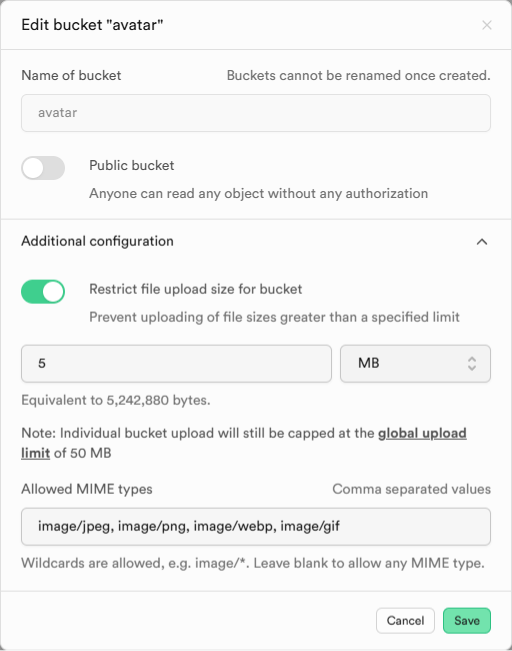
\includegraphics[width=0.55\textwidth]{files/Thomas/pics/Datenbank/storage/supabase_bucket_create.png}
\caption[Erstellen eines Buckets in Supabase]{Erstellen eines Buckets in Supabase}
\label{fig:supabase_bucket_create}
\end{figure}

Wie in Abbildung \ref{fig:supabase_bucket_create} zu sehen ist, wurde der Bucket so konfiguriert, dass nur Bilder mit einer maximalen Dateigröße von 5\,MB und ausschließlich Dateien im \texttt{image}- oder \texttt{gif}-Format hochgeladen werden dürfen.

Die Dateistruktur des Buckets ist wie folgt aufgebaut:

\begin{lstlisting}[style=mysql]
avatar/
 └── [user-id]/
      └── avatar.png
\end{lstlisting}

Somit kann jedem Benutzer ein individuelles Profilbild zugewiesen werden.

\newpage

\section{Auth}

Für die Authentifizierung wurde festgelegt, dass sich Benutzer mittels E-Mail und Passwort anmelden müssen.  
Bevor sich ein Benutzer jedoch anmelden darf, muss er zunächst seine E-Mail-Adresse verifizieren.  
Diese Funktion kann in den Supabase-Einstellungen aktiviert werden.  
Sobald ein Benutzer sich registriert, sendet Supabase automatisch eine Verifizierungs-E-Mail.

\begin{figure}[!htb]
\centering
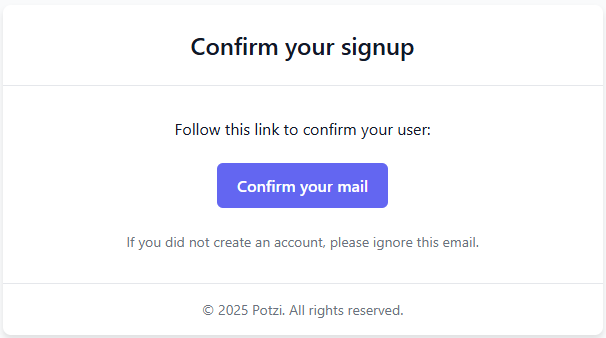
\includegraphics[width=0.75\textwidth]{files/Thomas/pics/Datenbank/auth/signup-email.png}
\caption[Supabase E-Mail-Verifizierung]{E-Mail-Verifizierung bei Supabase}
\label{fig:supabase_signup_email}
\end{figure}

Der Benutzer muss anschließend nur noch den Verifizierungslink in der E-Mail anklicken, um seine E-Mail-Adresse erfolgreich zu bestätigen.










\end{inhalt}

%Chapter 8 Website
\responsible{Thomas Potzmader} 
\begin{inhalt}
\renewcommand*\chapterpagestyle{scrheadings}
\chapter{Website}

Die Webseite wurde in \texttt{TypeScript} programmiert und verwendet \texttt{Next.js} als Framework.

\vspace{0.15cm}

Zum Starten des Projekts musste folgender Setup-Befehl ausgeführt werden:

\begin{lstlisting}[style=myconsole]
npx create-next-app@latest
\end{lstlisting}

Anschließend wurden die gewünschten Projekt-Einstellungen ausgewählt.  
Für dieses Projekt wurden folgende Optionen festgelegt:

\begin{lstlisting}[style=myconsole]
√ What is your project named? ... classscout
√ Would you like to use TypeScript? ... Yes
√ Would you like to use ESLint? ... Yes
√ Would you like to use Tailwind CSS? ... Yes
√ Would you like your code inside a `src/` directory? ... No
√ Would you like to use App Router? (recommended) ... Yes
√ Would you like to use Turbopack for `next dev`? ... Yes
√ Would you like to customize the import alias (`@/*` by default)? ... Yes
√ What import alias would you like configured? ... @/*
\end{lstlisting}



\newpage

\section{Signup}
\label{ref:Signup}
Für die Zuordnung der jeweiligen Benutzer ist es notwendig, dass sich die Nutzer einloggen können.  
Hierfür wurde eine Registrierkomponente erstellt, die den Registrier-Prozess ermöglicht.


\begin{figure}[!htb]
\centering
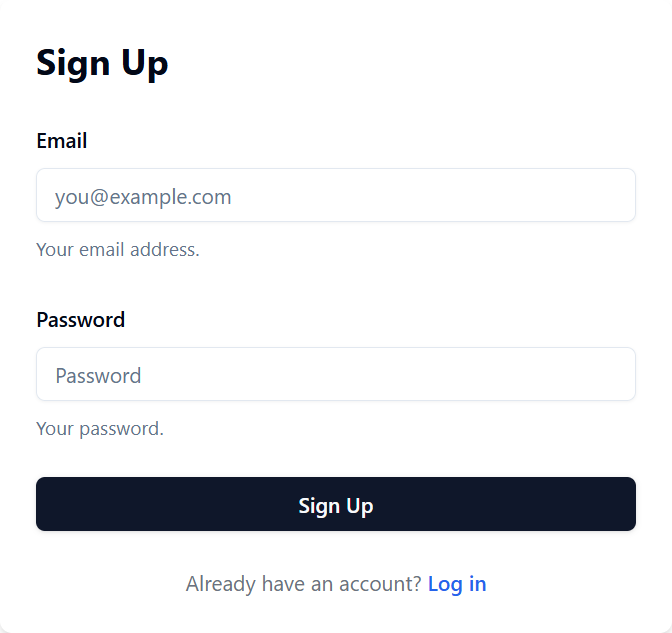
\includegraphics[width=0.5\textwidth]{files/Thomas/pics/Website/Signup/sign-up.png}
\caption[Bildbezeichnung für Abbildungsverzeichnis]{Registrierkomponente}
\label{fig:gehaeuse_internet_bild}
\end{figure}

Zur Validierung der Eingaben in den Feldern für \texttt{E-Mail} und \texttt{Passwort} wird die Bibliothek \textbf{Zod} verwendet. Dabei überprüft \textbf{Zod}, ob das E-Mail-Feld eine syntaktisch gültige E-Mail-Adresse enthält und ob das Passwortfeld einen String mit einer Mindestlänge von sechs Zeichen beinhaltet.


\begin{lstlisting}[style=mytsx]
const formSchema = z.object({
  email: z.string().email({
    message: "Please enter a valid email.",
  }),
  password: z.string().min(6, {
    message: "Password must be at least 6 characters.",
  }),
})
\end{lstlisting}
\index{Code Snippet 1@\hyperref[code:snippet1]{Snippet 1}}

\newpage

Für den Registrierungsvorgang wurde eine Funktion implementiert, die die eingegebene E-Mail-Adresse sowie das Passwort entgegennimmt und diese über eine Funktion des Supabase-Auth-Services im System registriert.


\begin{lstlisting}[style=mytsx]
export async function insert_user(email: string, password: string) {
  const supabase = await createClient();
  const { error } = await supabase.auth.signUp({
    email,
    password,
  });
  return error;
}
\end{lstlisting}

Nachdem der Nutzer erfolgreich registriert wurde, erfolgt eine Weiterleitung auf die Seite \texttt{/checkyouremails}, um ihn darüber zu informieren, dass er seine E-Mails überprüfen soll.

\begin{lstlisting}[style=mytsx]
      router.push("checkyouremails");
\end{lstlisting}

\subsection{Check Your Emails}

Auf dieser Seite wird überprüft, ob im Table \texttt{profiles} (siehe Referenz \ref{ref:profile-table-design}) das Feld \texttt{email\_confirmed\_at} gesetzt wurde und somit nicht mehr den Wert \texttt{null} enthält.  



\begin{figure}[H] 
  \centering
  \begin{subfigure}[b]{0.48\textwidth}
    \centering
    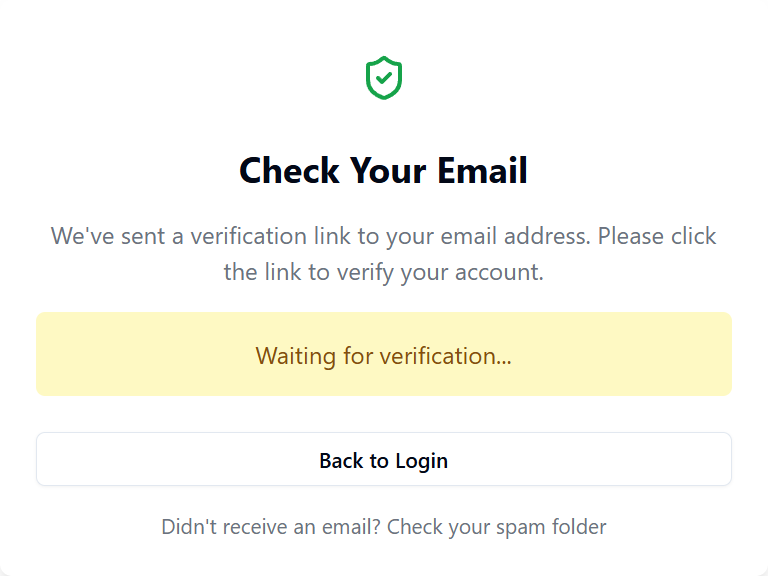
\includegraphics[width=1\textwidth]{files/Thomas/pics/Website/emailconfirmed/checkyouremails_waiting_verification.png}
    \caption{Email - Warte auf Verifikation}
    \label{fig:email_waiting_verification}
  \end{subfigure}
  \hfill
  \begin{subfigure}[b]{0.48\textwidth}
    \centering
    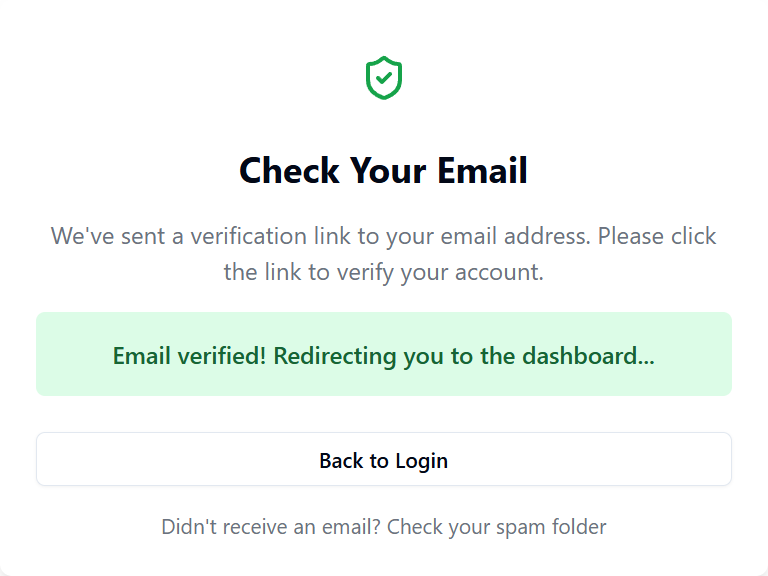
\includegraphics[width=1\textwidth]{files/Thomas/pics/Website/emailconfirmed/checkyouremails_verified.png}
    \caption{Email - Verifiziert}
    \label{fig:email_verified}
  \end{subfigure}
  \caption{Email Verifikation Status}
  \label{fig:email_verification_states}
\end{figure}


Dies geschieht über die Echtzeitfunktionalität von Supabase, welche es ermöglicht, Daten in Echtzeit zu aktualisieren und Änderungen in der Datenbank unmittelbar zu erkennen.

Sobald erkannt wird, dass die E-Mail-Adresse verifiziert wurde, erfolgt eine automatische Weiterleitung auf die \texttt{/login}-Seite.

\begin{lstlisting}[style=mytsx]
      router.push("/login");
\end{lstlisting}     


\section{Login}
\label{ref:Login}
Anschließend muss sich der Benutzer einloggen. Dieser Vorgang ist nahezu identisch mit dem Registrierungsprozess auf der \texttt{Sign-up}-Seite. 

\begin{figure}[!htb]
\centering
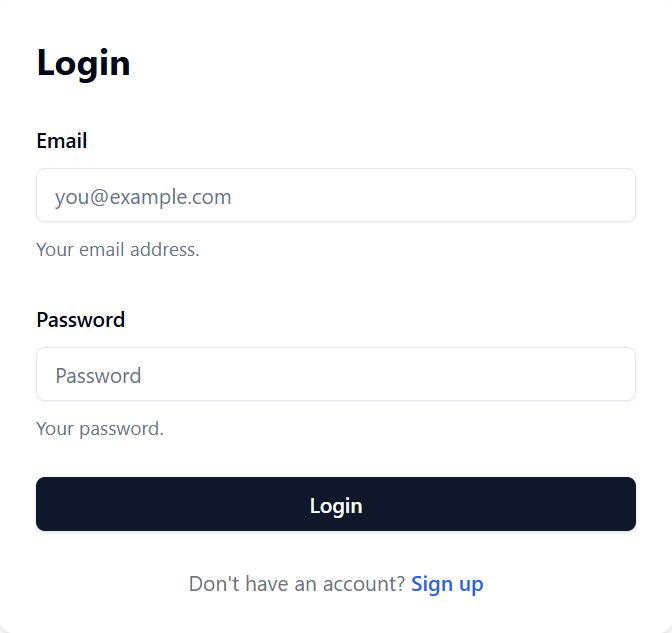
\includegraphics[width=0.5\textwidth]{files/Thomas/pics/Website/Login/login.png}
\caption[Bildbezeichnung für Abbildungsverzeichnis]{}
\label{fig:gehaeuse_internet_bild}
\end{figure}


Allerdings wird anstelle der \texttt{insert\_user}-Funktion zur Registrierung nun die \texttt{login\_user}-Funktion verwendet.
Da durch die E-Mail-Verifizierung keine automatische Benutzer-Session gestartet wird, muss der Benutzer sich manuell einloggen, um eine Session zu starten.

\begin{lstlisting}[style=mytsx]
export async function login_user(email: string, password: string) {
  const supabase = await createClient();
  const { error } = await supabase.auth.signInWithPassword({
    email,
    password,
  });
  return error;
}
\end{lstlisting}

\clearpage

\newpage

\section{Setup Profile}

Wenn ein Benutzer versucht, auf die \texttt{/setup-profile}-Seite zuzugreifen, und bereits angemeldet ist, wird überprüft, ob im Profil entweder der Benutzername, der Vorname oder der Nachname fehlt.  
Falls einer dieser Werte nicht gesetzt ist, wird der Benutzer automatisch durch die Middleware (siehe \ref{ref:middelware}) auf die entsprechende Seite weitergeleitet.

\vspace{0.25cm}

Die \texttt{/setup-profile}-Seite dient dazu, sicherzustellen, dass jeder Benutzer einen Benutzernamen, einen Vornamen und einen Nachnamen angegeben hat und diese Informationen vollständig vorliegen.

\begin{figure}[!htb]
\centering
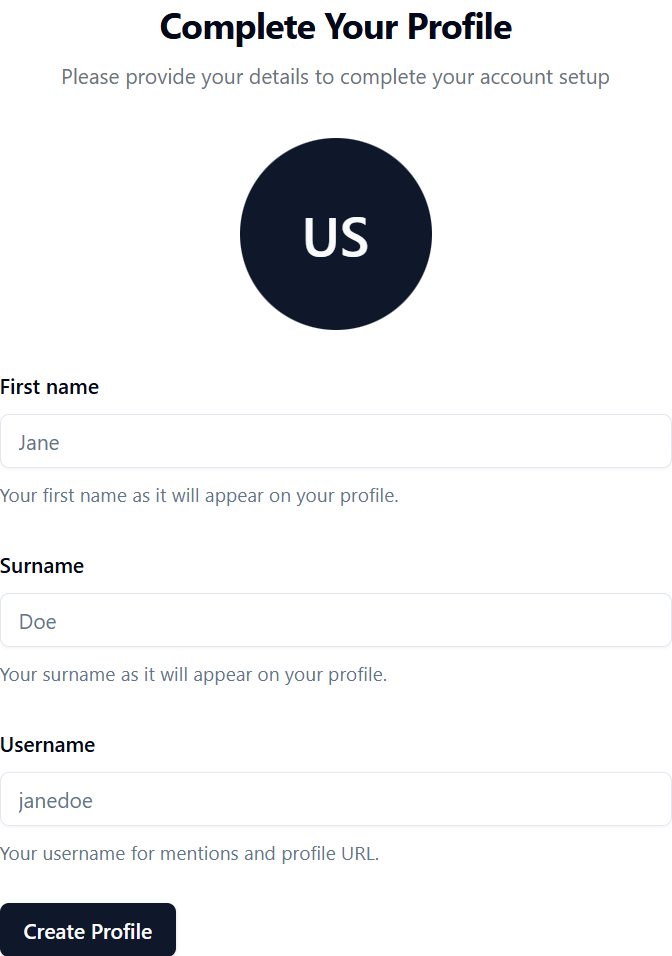
\includegraphics[width=0.55\textwidth]{files/Thomas/pics/Website/setup-profile/setup-profile.png}
\caption[Bildbezeichnung für Abbildungsverzeichnis]{}
\label{fig:gehaeuse_internet_bild}
\end{figure}

\clearpage

Diese Seite besteht ebenfalls aus einer Komponente, die ähnlich zur \texttt{Login}- und \texttt{Signup}-Komponente aufgebaut ist (siehe \ref{ref:Signup}, \ref{ref:Login}).

Der wesentliche Unterschied zwischen dem \texttt{Login}-Formular und der \texttt{Setup-Profile}-Seite besteht darin, dass auf der \texttt{Setup-Profile}-Seite zusätzlich ein Avatar hinzugefügt oder gelöscht werden kann.

\begin{lstlisting}[style=mytsx]
<AvatarUpload
    userName={form.getValues("first_name") || "User"}
    userId={userId || undefined}
    onImageChange={handleImageChange}
/>
\end{lstlisting}

\newpage

\subsection{AvatarUpload-Komponente}

Die \texttt{AvatarUpload}-Komponente stellt ein zentrales Element der Benutzerprofilseite (\texttt{/setup-profile}) dar. Sie ermöglicht eine intuitive Verwaltung von Profilbildern. Die Komponente implementiert vier Kernfunktionalitäten:

\vspace{0.75cm}

\textbf{Hochladen eines neuen Avatars mit Live-Vorschau}

\vspace{0.15cm}

Die Komponente ermöglicht das Hochladen von Profilbildern mit sofortiger Vorschau. Der Prozess umfasst:
\begin{itemize}
    \item Dateiauswahl aus dem lokalen Dateisystem
    \item Automatische Validierung (max. 5MB, nur Bildformate)
    \item Sofortige Vorschau ohne direkten Server-Upload
\end{itemize}


\begin{lstlisting}[style=mytsx, caption={Implementierung des Avatar-Uploads mit Validierung}, label={lst:avatar_upload}]
const handleFileSelect = async (event: React.ChangeEvent<HTMLInputElement>) => {
  const file = event.target.files?.[0];
  if (!file || !validateFile(file)) return;

  try {
    const fileExtension = file.type === "image/jpeg" ? "jpg" : "png";
    const standardizedFile = new File(
      [file], 
      `avatar.${fileExtension}`, 
      { type: file.type }
    );
    const previewUrl = URL.createObjectURL(file);

    setState(prev => ({
      ...prev,
      selectedFile: standardizedFile,
      previewUrl,
      avatarAction: "upload"
    }));
  } catch (error) {
    toast({
      title: "Fehler",
      description: "Datei konnte nicht verarbeitet werden."
    });
  }
};
\end{lstlisting}

\textbf{Entfernen bestehender Avatare}
\vspace{0.15cm}
Ein vorhandenes Profilbild kann über eine dedizierte Schaltfläche entfernt werden:
\begin{itemize}
    \item Visuelles Feedback durch \texttt{X}-Symbol
    \item Sofortige Aktualisierung der Anzeige
    \item Markierung zur Löschung beim nächsten Speichervorgang
\end{itemize}

\begin{lstlisting}[style=mytsx, caption={Implementierung der Avatar-Löschung}, label={lst:avatar_delete}]
const handleRemoveAvatar = async () => {
  try {
    setState(prev => ({
      ...prev,
      selectedFile: null,
      previewUrl: null,
      avatarAction: "delete"
    }));
    
    window.dispatchEvent(new CustomEvent("avatarChanged", {
      detail: { userId, action: "delete" }
    }));
  } catch (error) {
    toast({
      title: "Fehler",
      description: "Avatar konnte nicht entfernt werden."
    });
  }
};
\end{lstlisting}

\subsubsection{Intelligente Fallback-Darstellung}
Bei fehlendem Profilbild generiert die Komponente automatisch einen visuellen Platzhalter:
\begin{itemize}
    \item Extraktion der Benutzerinitialen aus dem Namen
    \item Konsistente Darstellung im UI-Design
    \item Automatische Anpassung an verschiedene Namensformate
\end{itemize}

\begin{lstlisting}[style=mytsx, caption={Generierung der Fallback-Initialen}, label={lst:avatar_initials}]
const getInitials = (name: string): string => {
  if (!name) return "??";
  const parts = name.split(" ");
  return parts.length === 1
    ? parts[0].substring(0, 2).toUpperCase()
    : (parts[0].charAt(0) + parts[parts.length - 1].charAt(0)).toUpperCase();
};
\end{lstlisting}

\subsubsection{Echtzeit-Synchronisation}
Die Komponente nutzt Supabase Realtime für die Live-Synchronisation:
\begin{itemize}
    \item Automatische Aktualisierung bei externen Änderungen
    \item Effiziente Subscription-Verwaltung
    \item Robuste Fehlerbehandlung
\end{itemize}

\begin{lstlisting}[style=mytsx, caption={Implementierung der Echtzeit-Synchronisation}, label={lst:avatar_subscription}]
useEffect(() => {
  if (!userId) return;
  
  let mounted = true;
  const setupSubscription = async () => {
    try {
      const channel = await subscribeToAvatarChanges(userId, () => {
        if (mounted) refreshAvatar();
      });
      if (mounted) channelRef.current = channel;
    } catch (error) {
      console.error("Subscription fehlgeschlagen:", error);
    }
  };

  setupSubscription();
  return () => {
    mounted = false;
    if (channelRef.current) unsubscribe(channelRef.current);
  };
}, [userId]);
\end{lstlisting}

Die \texttt{AvatarUpload}-Komponente vereint somit moderne Webtechnologien mit benutzerfreundlicher Funktionalität und robuster Fehlerbehandlung. Durch die Verwendung von TypeScript und React-Hooks wird eine wartbare und typsichere Implementierung gewährleistet.







\newpage

\section{Middleware}
\label{ref:middelware}

Die Datei \texttt{middleware} ist ein zentraler Bestandteil der Anwendung und wird bei jedem Seitenaufruf ausgeführt.  
\vspace{0.15cm}

Sie übernimmt wichtige Aufgaben im Bereich Sicherheit, Weiterleitung und Zustandskontrolle der Anwendung.  

\vspace{2cm}

\begin{figure}[!htb]
\centering
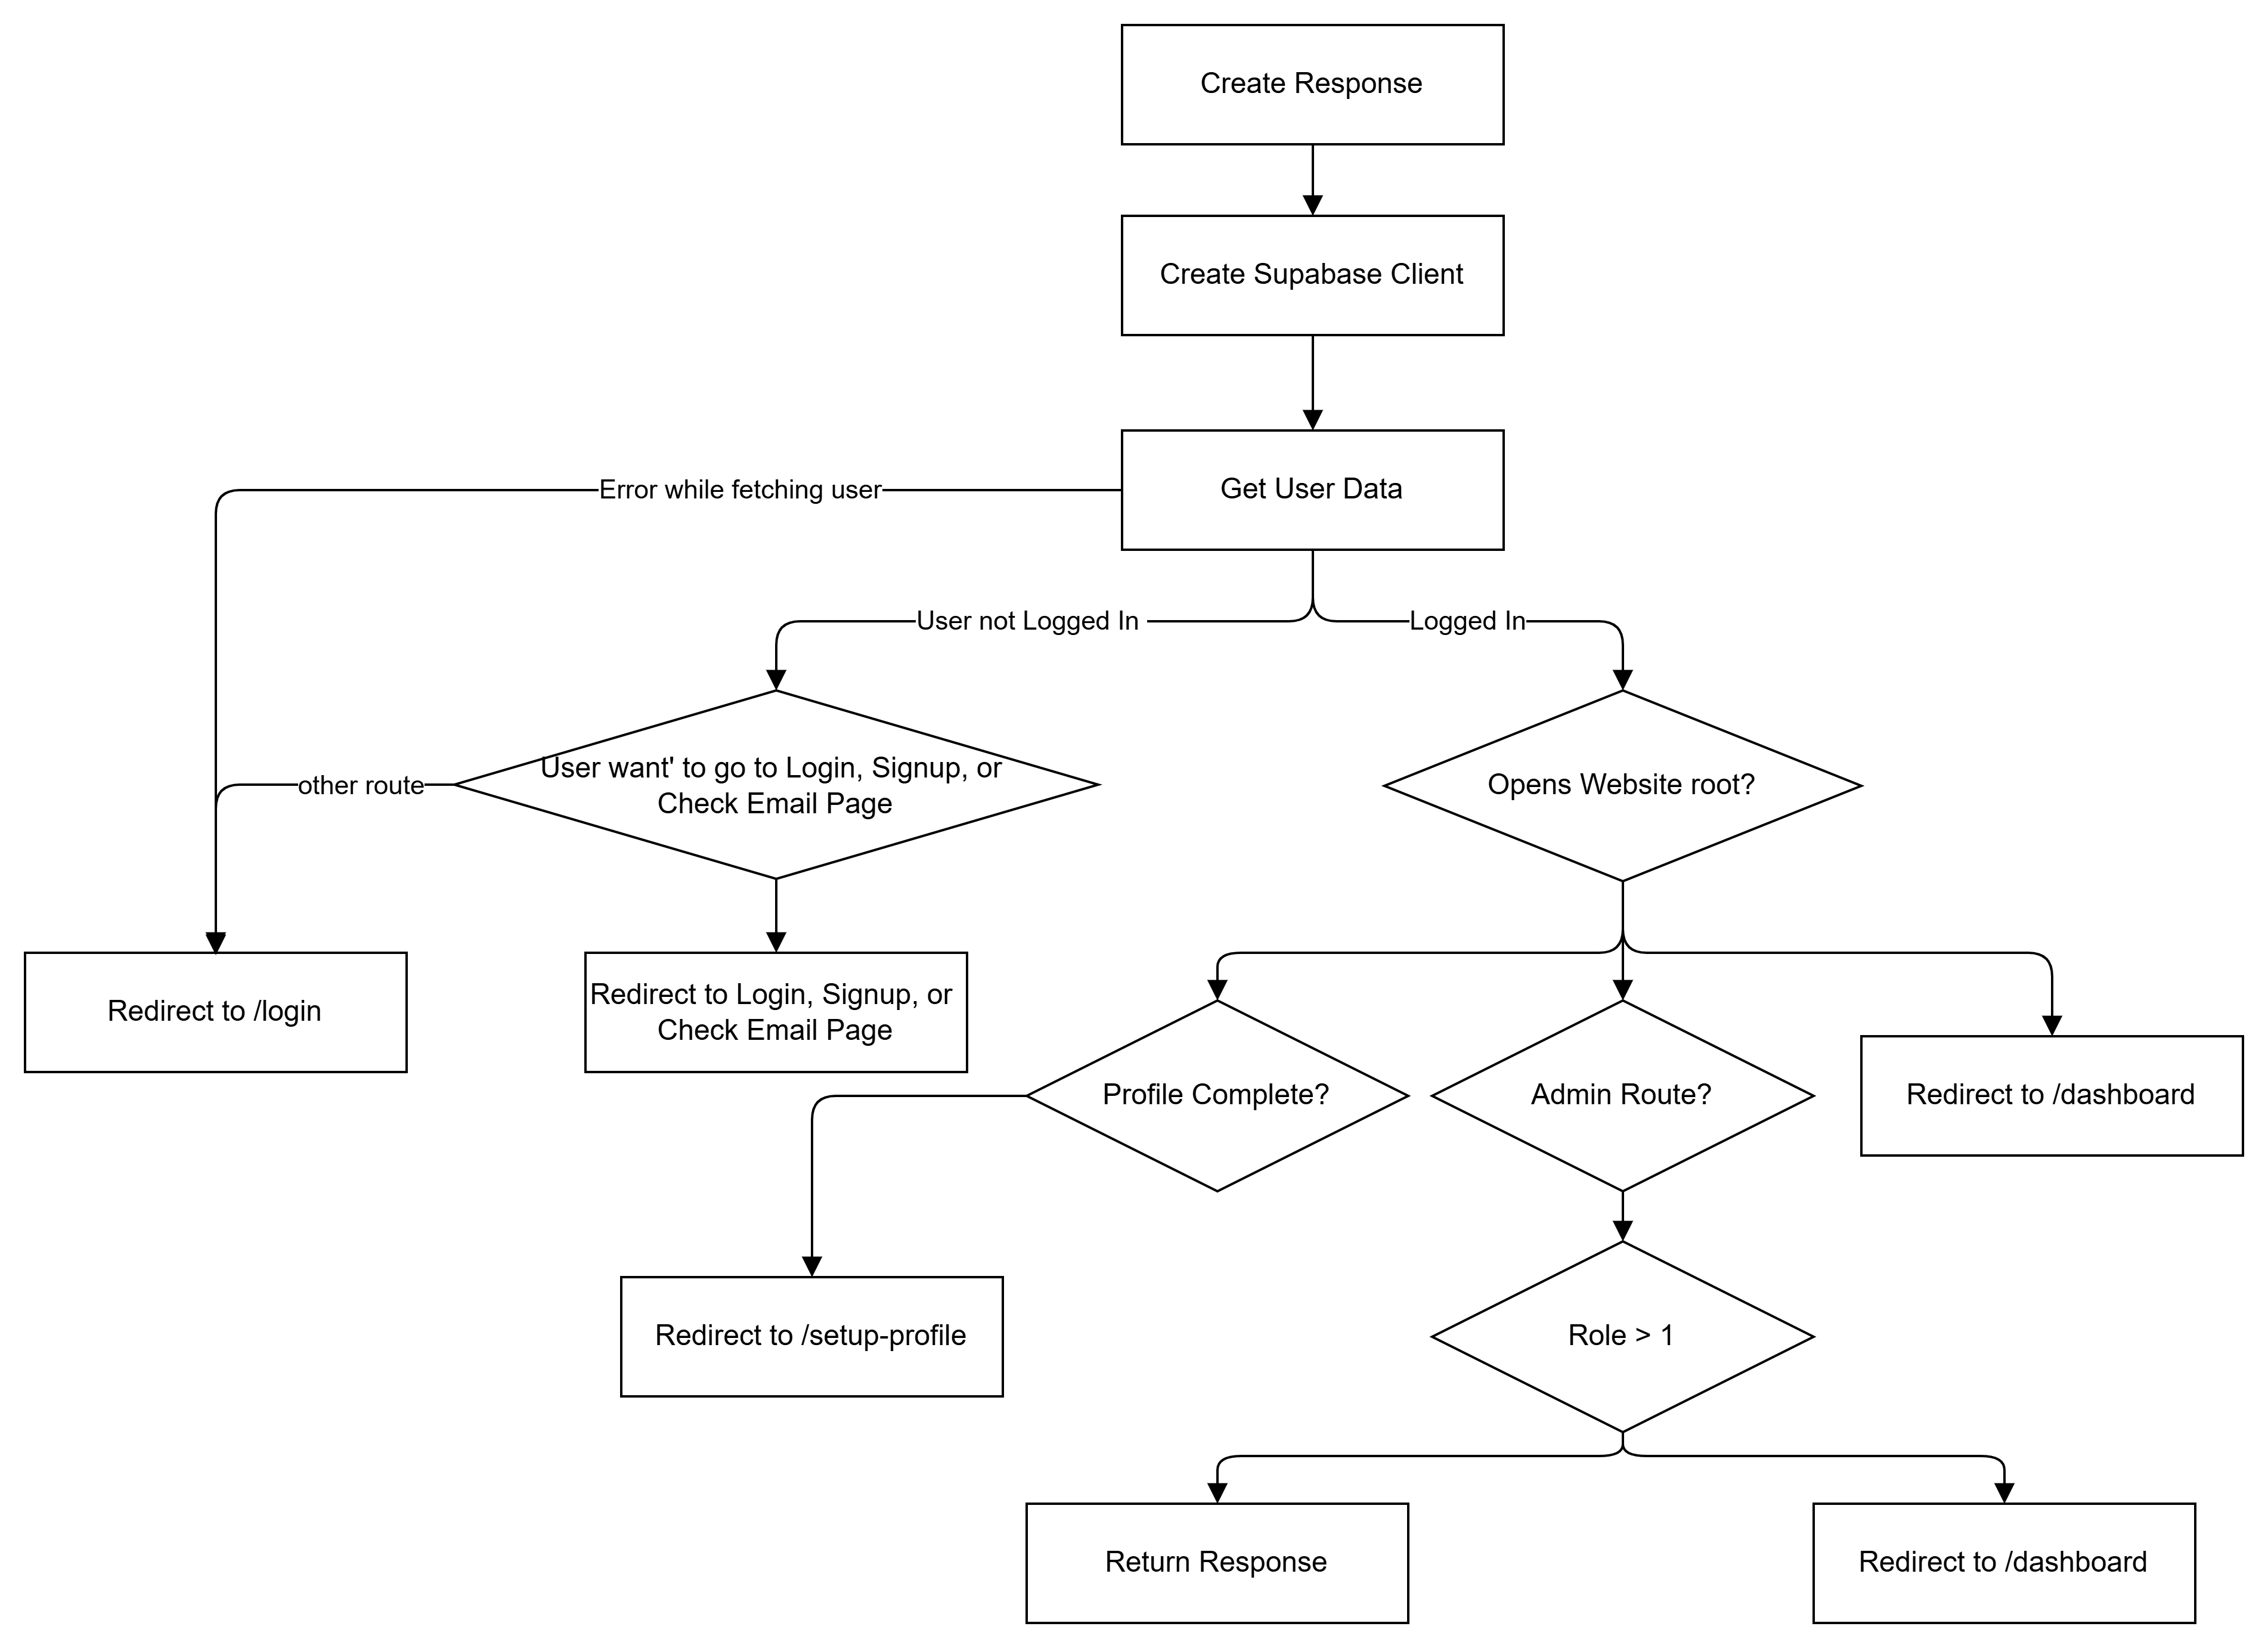
\includegraphics[width=1\textwidth]{files/Thomas/pics/Website/middelware/middelware.png}
\caption[Bildbezeichnung für Abbildungsverzeichnis]{Flowchart von der Middelware}
\label{fig:middleware}
\end{figure}

\newpage

Die Middleware wird automatisch bei jedem Aufruf einer Seite ausgeführt, sofern der aufgerufene Pfad nicht explizit ausgeschlossen wurde.  
Dadurch lassen sich serverseitige Logiken zentral abbilden, wie z.\,B. Authentifizierungsprüfungen, Weiterleitungen oder Cookie-Handling.

\subsection*{Wichtige Funktionen der Middleware}

\begin{enumerate}[label=\textbf{\arabic*.}]
  \item \textbf{Authentifizierung und Autorisierung}
  \begin{itemize}
    \item Überprüfung, ob ein Benutzer eingeloggt ist, mittels \texttt{supabase.auth.getUser()}
    \item Nicht eingeloggte Benutzer werden zur Login-Seite weitergeleitet
    \item Eingeloggte Benutzer, die sich auf Auth-Seiten befinden (z.\,B. \texttt{/login}, \texttt{/signup}), werden automatisch zum Dashboard umgeleitet
  \end{itemize}

  \item \textbf{Profilüberprüfung}
  \begin{itemize}
    \item Die Middleware prüft, ob das Benutzerprofil vollständig ist (Vorname, Nachname, Benutzername)
    \item Bei unvollständigem Profil erfolgt eine Weiterleitung zur \texttt{/setup-profile}-Seite
  \end{itemize}

  \item \textbf{Admin-Berechtigungen}
  \begin{itemize}
    \item Für Admin-Routen (\texttt{/admin/*}) wird geprüft, ob der Benutzer die Rolle \texttt{admin} besitzt
    \item Andernfalls erfolgt eine automatische Weiterleitung zum Dashboard
  \end{itemize}

  \item \textbf{Cookie-Management}
  \begin{itemize}
    \item Es werden Standard-Cookies wie \texttt{theme} und \texttt{activeSchool} gesetzt
    \item Die Authentifizierung erfolgt mithilfe des Supabase-Cookie-Managements
  \end{itemize}

\newpage

  \item \textbf{Routing-Logik}
  Die Routing-Logik prüft anhand des Authentifizierungsstatus, ob ein Benutzer weitergeleitet werden muss:


\begin{lstlisting}[style=mytsx]
  if (!user) {
    // If user is not logged in
    const isAuthRoute = path === '/login' || 
                        path === '/signup' || 
                        path === '/checkyouremails'
    
    if (!isAuthRoute) {
      // Redirect unauthenticated users to login page
      const redirectUrl = new URL('/login', request.url)
      return NextResponse.redirect(redirectUrl)
    }
  } else {
    // If user is logged in
    const isAuthRoute = path === '/login' || 
                        path === '/signup' || 
                        path === '/'
    
    if (isAuthRoute) {
      // Redirect authenticated users to dashboard
      const redirectUrl = new URL('/dashboard', request.url)
      return NextResponse.redirect(redirectUrl)
    }

  \end{lstlisting}

  \item \textbf{Matcher-Konfiguration}
  Die \texttt{matcher}-Konfiguration legt fest, auf welchen Routen die Middleware ausgeführt werden soll in diesen Falle auf fast alle:

\begin{lstlisting}[language=TypeScript]
matcher: [
  '/((?!_next/static|_next/image|favicon.ico|public/|api/|.
  *\\.(?:svg|png|jpg|jpeg|gif|webp|js|css)$).*)',
]


\end{lstlisting}



\clearpage

\newpage

\section{Seitenleiste}

Die Seitenleiste ist für die Navigation zwischen den verschiedenen Klassen, Abteilungen und Schulen verantwortlich.  

Der Aufbau der Seitenleiste besteht aus den folgenden Komponenten:

\begin{itemize}
    \item school-swticher (SidebarHeader)
    \item nav-departments-classes-devices (SidebarContent)
    \item nav-user (SidebarFooter)
\end{itemize}

%%% Bild einfügen von der Struktur

\vspace{2cm}

\begin{figure}[!htb]
\centering
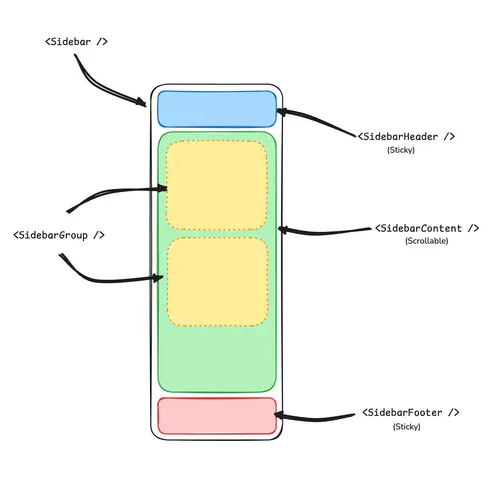
\includegraphics[width=1\textwidth]{files/Thomas/pics/Website/Sidebar/sidebar-aufbau.png}
\caption[Bildbezeichnung für Abbildungsverzeichnis]{}
\label{fig:gehaeuse_internet_bild}
\end{figure}

\newpage

\subsection{School-Switcher}

Die \texttt{school-switcher}-Komponente dient dazu, die aktuelle Schule auszuwählen bzw. zu wechseln.

\begin{figure}[!htb]
\centering

\includegraphics[width=1\textwidth]{files/Thomas/pics/Website/Sidebar/school-switcher/school-switcher.png}
\caption[School-Switcher Komponente geschlossen]{School-Switcher Komponente im geschlossenen Zustand}
\label{fig:school_switcher_closed}
\end{figure}

Administratoren können über einen Klick auf die Komponente ein Auswahlfenster öffnen, in dem sie zwischen den verfügbaren Schulen wählen können.  
Schüler, Lehrer und Direktoren besitzen hingegen keine Berechtigung, die Schule zu ändern.

\begin{figure}[!htb]
\centering
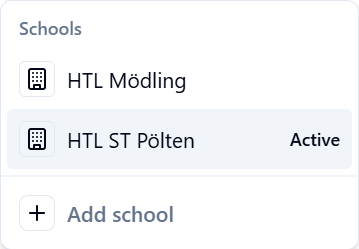
\includegraphics[width=0.75\textwidth]{files/Thomas/pics/Website/Sidebar/school-switcher/school-switcher-open.png}
\caption[School-Switcher geöffnet]{School-Switcher Komponente im geöffneten Zustand}
\label{fig:school_switcher_open}
\end{figure}

Die ausgewählte Schule wird anschließend in einem Cookie gespeichert, um beim nächsten Aufruf der Webseite automatisch wiederhergestellt zu werden.  
Im folgenden Codebeispiel wird das Cookie clientseitig unter dem Namen \texttt{activeSchool} gesetzt und speichert die \texttt{UUID} der Schul-ID.

\begin{lstlisting}[language=TypeScript]
Cookies.set('activeSchool', school.id, {
    secure: process.env.NODE_ENV === 'production',
    sameSite: 'lax',
    path: '/',
});
\end{lstlisting}

Das Attribut \texttt{secure} sorgt dafür, dass das Cookie nur über HTTPS gesendet wird.  
Da dies jedoch nur in der Produktionsumgebung erforderlich ist, wird die Einstellung über \texttt{process.env.NODE\_ENV} gesteuert.  
Durch die Einstellung \texttt{sameSite = lax} wird das Cookie nur bei normaler Navigation und GET-Anfragen mitgesendet.  
Der Parameter \texttt{path} legt fest, dass das Cookie auf der gesamten Webseite verfügbar ist.


%%% ADD School maby









\subsection{nav-departments-classes-devices}


\begin{figure}[!htb]
\centering
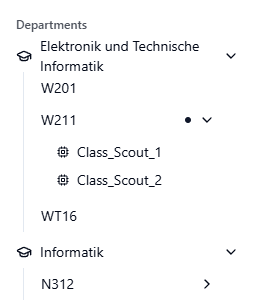
\includegraphics[width=0.5\textwidth]{files/Thomas/pics/Website/Sidebar/nav-departments-classes-devices/nav-screen.png}
\caption[Bildbezeichnung für Abbildungsverzeichnis]{}
\label{fig:gehaeuse_internet_bild}
\end{figure}



Die Aufgabe der nav-departments-classes-devices Komponente ist das Man zwischen den Abteilungen Klassen und Sensoren umher Navigiren kann. Damit erkannt wird in welcher Schule man sich Befindet wurde eine Speziele URL Addresse entworden:

\begin{lstlisting}[language=mytsx]

domainname/uuid-der-schule/dashboard?department=uuid-in dem-Department-man-gerae-ist&class=uuid-in-welcher-Klasse-man-sich-gerade befindet&device=device-uuid

Beispiel

domainname/0d3e37cf-8350-46f2-823b-26dd90c01266/dashboard?department=e1ed2bd8-4c9c-40f8-bec7-4edcebe59fc1&class=eb4355fd-1e98-4961-be62-36fa9fc5cec0&device=a52eb8dc-5df5-475a-8a9f-f5f5a24ac2d3
\end{lstlisting}


%%% gehört vlt noch was hin 

\subsection{nav-user}

Die nav-user Komponente ist im SidebarFooter(Am Boden der Seitenleiste). Sie ist verantwortlich dafür das sie vom Benutzer den Benutzernamen die E-Mail Addresse den Avatar anzeigt

\begin{figure}[!htb]
\centering

\includegraphics[width=0.5\textwidth]{files/Thomas/pics/Website/Sidebar/nav-user/user-component.png}
\caption[Bildbezeichnung für Abbildungsverzeichnis]{}
\label{fig:gehaeuse_internet_bild}
\end{figure}


Außerdem ist es auch noch da um Auf den Profil Editor des Benutzers zu kommen. Wenn man ein Admin ist kann man auch auf die Administrator Seiten der Website kommen und es gibt noch eine Settings Seite und einen Logout Knopf um sich abzumelden. 

\begin{figure}[!htb]
\centering
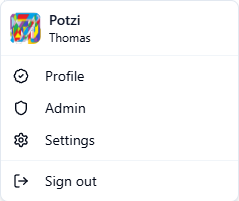
\includegraphics[width=0.5\textwidth]{files/Thomas/pics/Website/Sidebar/nav-user/user-component-open.png}
\caption[Bildbezeichnung für Abbildungsverzeichnis]{}
\label{fig:gehaeuse_internet_bild}
\end{figure}



Beim Abmelden von der Seite wird als erstes  gewarted bis die signOut funktion ein success zurück bekommt danach wird der user auf die Login seite weitergeleitet. 

\begin{lstlisting}[language=mytsx]
  const handleSignOut = async () => {
    const { success, error } = await signOut();
    if (success) {
      router.push("/login");
    } else {
      console.error("Error signing out:", error);
    }
  };
\end{lstlisting}


\newpage

\section{Settings Seite}

\begin{figure}[!htb]
\centering
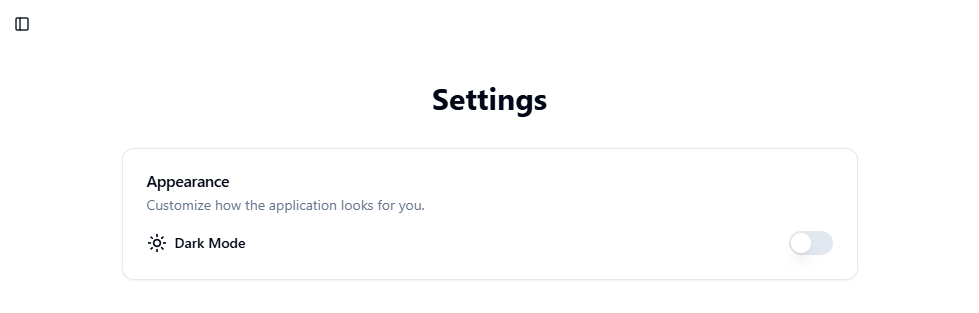
\includegraphics[width=1\textwidth]{files/Thomas/pics/Website/Settings/settings-screen.png}
\caption[Bildbezeichnung für Abbildungsverzeichnis]{}
\label{fig:gehaeuse_internet_bild}
\end{figure}


Die Settings(Einstellungs Seite hat nur eine Aufgabe und zwar den Theme zu wechseln dieser wird dann wieder in den Cookies gespeichet mit den Namen theme um bei einen Refresh nicht den Theme zu verlieren.

\vspace{2cm}

In diesem Code wird ein Schalter eingesetzt, um zwischen dem Dunklen Modus und dem Hellen Modus zu wechseln. Dieser Switch hat die ID \texttt{dark-mode} und eine Variable, die den Wert des Schalters annimmt. Am Schluss wird jedes Mal, wenn der Schalter betätigt wird, die Funktion \texttt{toggleTheme()} aufgerufen, um die Cookies zu setzen und das Theme der Seite zu verändern.


\begin{lstlisting}[language=mytsx]
<Switch
    id="dark-mode"
    checked={isDarkMode}
    onCheckedChange={toggleTheme}
  />
\end{lstlisting}

\newpage

\section{Profile Seite}

Die Profile Seite ist eigetnlich die Profile-Setup Seite um den Benutzer die Möglichkeit zu geben das Profil Bild den Vorname Nachnmaen und Bentuzernamen zu aktualisieren.


\begin{figure}[!htb]
\centering
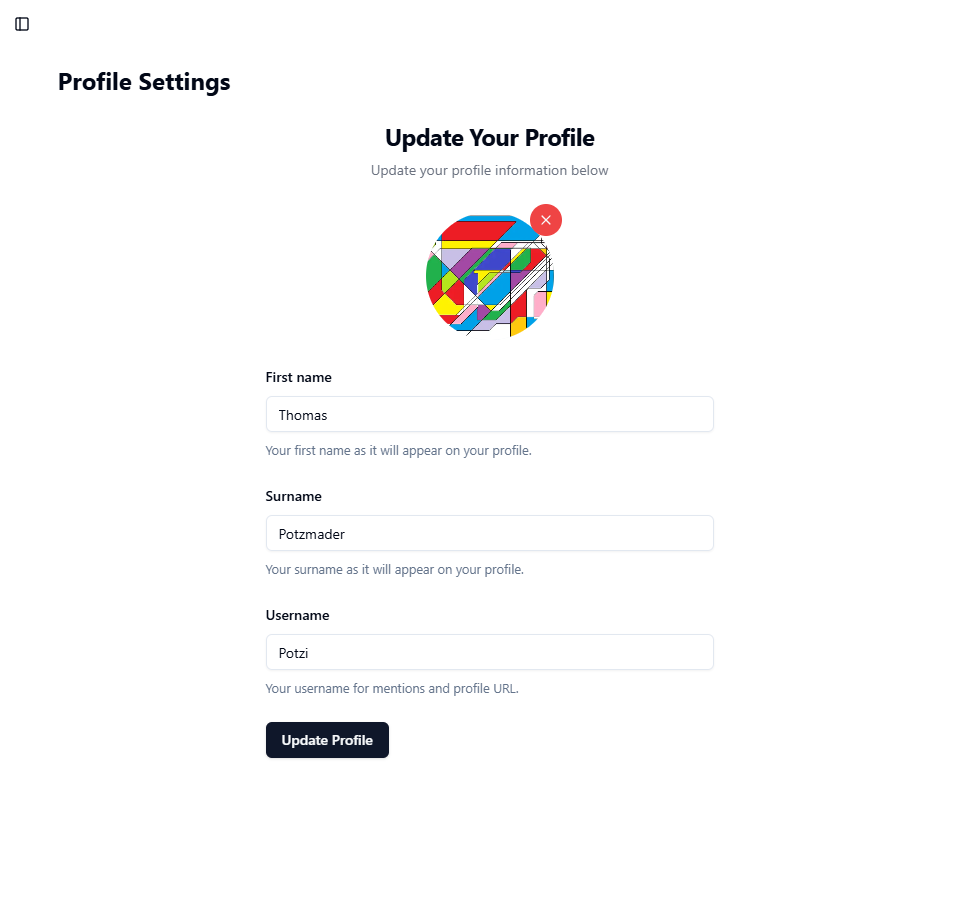
\includegraphics[width=1\textwidth]{files/Thomas/pics/Website/Profile/profile-screen.png}
\caption[Bildbezeichnung für Abbildungsverzeichnis]{}
\label{fig:gehaeuse_internet_bild}
\end{figure}

\newpage

\section{Admin Dashboard}

Das Admin Dashboard ist dafür da um alle User, Geräte, Klassen, Abteilungen und Schulen zu Erstellen oder zu Löschen. 

\begin{figure}[!htb]
\centering
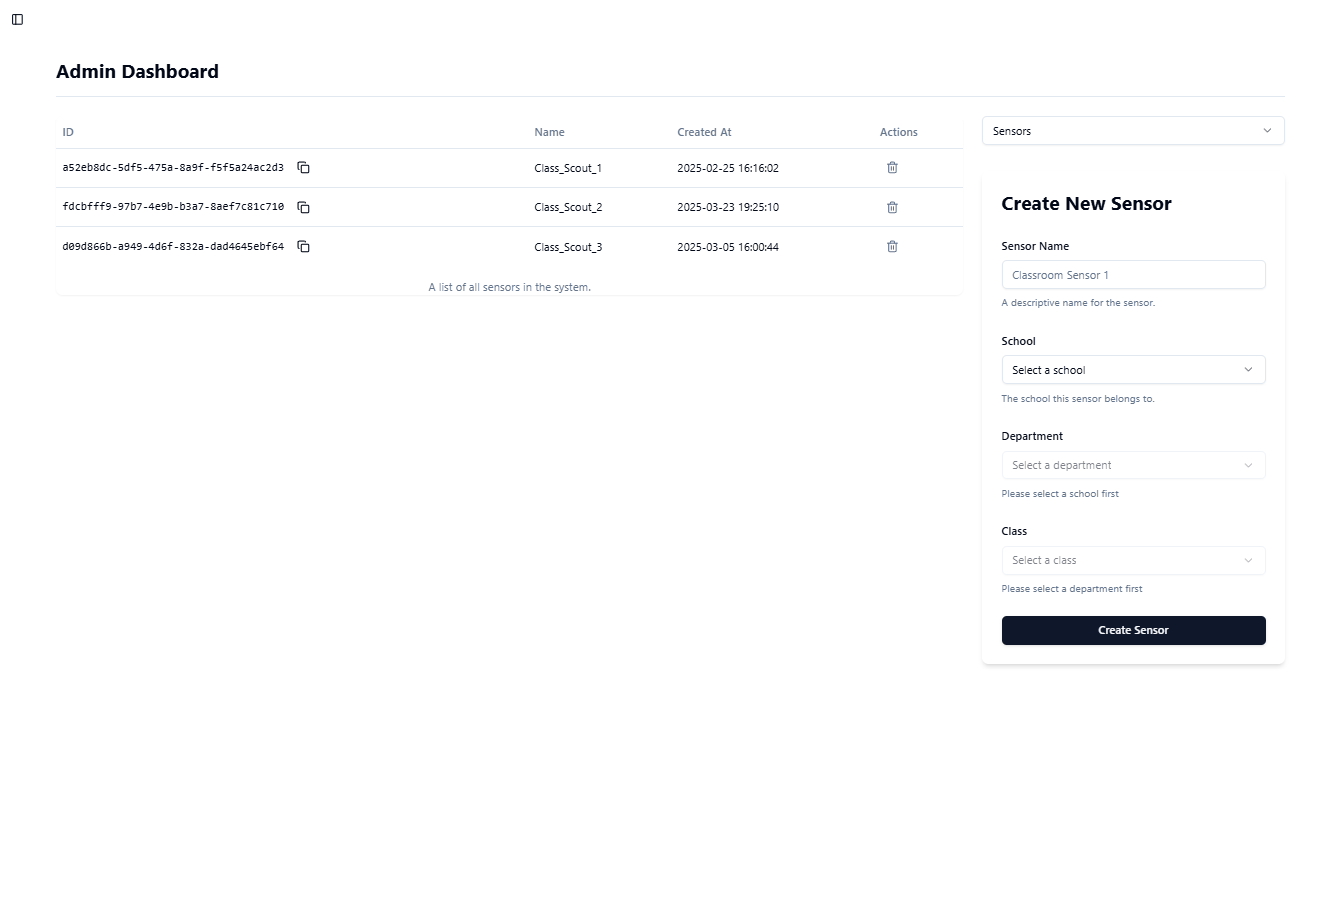
\includegraphics[width=1\textwidth]{files/Thomas/pics/Website/admin/devices/devices-screen.png}
\caption[Bildbezeichnung für Abbildungsverzeichnis]{}
\label{fig:gehaeuse_internet_bild}
\end{figure}

\clearpage


In dem Bild kann man sehen wie das Dashboard der Sensoren ausschaut.

\subsection{Table}

Jeder Table hat außer die User Table die ist speziel hat am anfag die uuid von den Strukturelementen. Diese Last sich immer ganz einfach kopiern durch einen Button. Danach wird der Name angezeigt und nachdem wird der Zeitpunkt der Erstellung des Strukturelementes angeziegt und am schluss eine Möglichkeit diese Strukturelemente zu löschen. 

\begin{figure}[!htb]
\centering
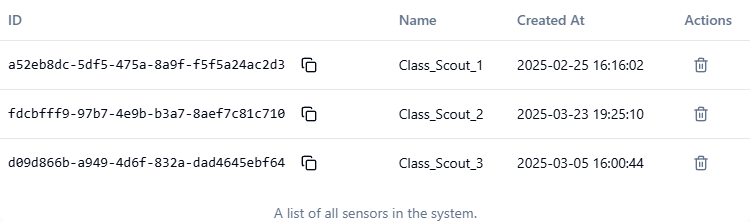
\includegraphics[width=1\textwidth]{files/Thomas/pics/Website/admin/sensors/sensor-table.png}
\caption[Bildbezeichnung für Abbildungsverzeichnis]{}
\label{fig:gehaeuse_internet_bild}
\end{figure}

Zum Kopieren des Textes wird der Inhalt zunächst in die Zwischenablage (\texttt{clipboard}) gespeichert mit der funktion \texttt{navigator.clipboard.writeText(value)}. 
Anschließend wird die Variable \texttt{isCopied} auf \texttt{true} gesetzt, wodurch das anzuzeigende Icon entsprechend geändert wird.  
Nach zwei Sekunden wird die Variable wieder auf \texttt{false} zurückgesetzt, um das Icon erneut zu aktualisieren.


\begin{lstlisting}[language=mytsx]
const copy = async () => {
    try {
      await navigator.clipboard.writeText(value);
      setIsCopied(true);
      setTimeout(() => setIsCopied(false), 2000);
    } catch (err) {
      console.error("Failed to copy text: ", err);
    }
  };
\end{lstlisting}
%%% code hinzufügen 

\clearpage

\subsection{Erstellen}

Beim Erstellen von den Verschieden Strukturelementen wurde eine immer die Selbe Struktur genommen. Oben Wird immer der Name eingegeben danch kommen die abhängigen slektoren.

\begin{figure}[!htb]
\centering
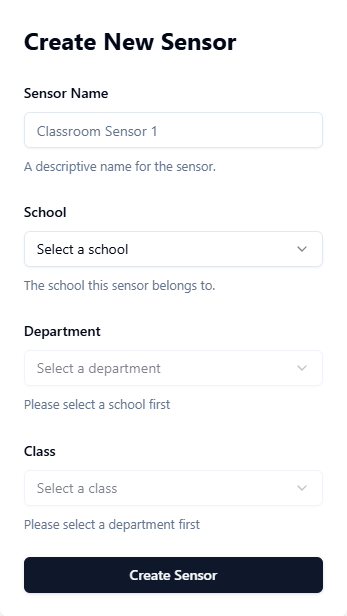
\includegraphics[width=0.8\textwidth]{files/Thomas/pics/Website/admin/sensors/sensor-create.png}
\caption[Bildbezeichnung für Abbildungsverzeichnis]{}
\label{fig:sensor-create}
\end{figure}

Bei den Beispiel für die Sensor-Erstellungs Komponente \ref{fig:sensor-create} kann man sehen das diese die Schule, Abeteilung und die Klasse benötigt da sie von diesen Parametern abhängig ist.

\newpage

\textbf{Schule automatische Vervollständigung}

Für das Erstellen von Schulen wurde eine Auto Vervollständigung von Google bentutz um leichter den Standort der Schulen einzugeben.

\textbf{Validierung der Autocomplete-Eingabe}

In diesem Code-Snippet wird geprüft, ob der eingegebene Text mindestens 3 Zeichen lang ist und der \texttt{autocompleteService} verfügbar ist. Wenn dies der Fall ist, werden über die Google Places API passende Vorschläge abgefragt.

\begin{itemize}
    \item Falls Ergebnisse gefunden wurden, werden diese in den State \texttt{predictions} geladen.
    \item Falls keine Ergebnisse vorhanden sind (\texttt{ZERO\_RESULTS}), wird eine leere Liste angezeigt und eine Fehlermeldung gesetzt.
    \item Bei allen anderen Fehlern wird ebenfalls eine leere Liste angezeigt und eine allgemeine Fehlermeldung angezeigt.
    \item Nach der Verarbeitung wird der Ladezustand auf \texttt{false} gesetzt.
\end{itemize}

\vspace{0.5cm}

\begin{lstlisting}[language=mytsx]
if (inputValue.length > 2 && autocompleteService.current) {
    autocompleteService.current.getPlacePredictions(
        { input: inputValue },
        (predictions, status) => {
            if (status === window.google.maps.places.PlacesServiceStatus.OK && predictions) {
                setPredictions(predictions);
            } else if (status === window.google.maps.places.PlacesServiceStatus.ZERO_RESULTS) {
                setPredictions([]);
                setError("No results found");
            } else {
                setPredictions([]);
                setError("Error fetching predictions");
            }
            setLoading(false);
        },
    );
} else {
    setPredictions([]);
    setLoading(false);
}
\end{lstlisting}

\clearpage

\subsection{Schule Map}


\begin{figure}[!htb]
\centering
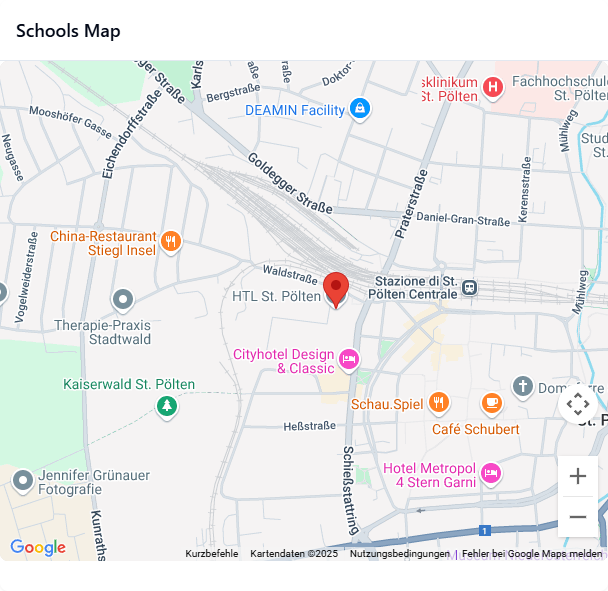
\includegraphics[width=0.8\textwidth]{files/Thomas/pics/Website/admin/school/school-map.png}
\caption[Bildbezeichnung für Abbildungsverzeichnis]{Google Maps Karte auf der Webseite}
\label{fig:gehaeuse_internet_bild}
\end{figure}

Die Schule Map ist eine Google Maps karte den Standort
der Schulen anzeigen kann.

\vspace{1cm}


In diesen Komponent wurde die Map von react-google-maps/api genommen diese erlaubt für viele Eisntellungen aber sie ist auch leicht tu implementiren

\vspace{0.15cm}

In diesen code wird die Map Eingetsellt der Standard Ort wo die Map reingezoomed ist in St Pölten
Außerdem wruden viele Controle Eisntellungen auf falsch gesstellt da der User nur die Map zum Zoomen benutzen soll und zu schauen wo Schulen sind.


\begin{lstlisting}[language=mytsx]
<GoogleMap
        mapContainerStyle={containerStyle}
        center={defaultCenter}
        zoom={defaultZoom}
        options={{
          disableDefaultUI: false,
          zoomControl: true,
          mapTypeControl: false,
          streetViewControl: false,
          fullscreenControl: false,
        }}
      >
\end{lstlisting}





\clearpage

\section{Dashbaord}

Das Dashboard ist der Kern punkt dieser Diplomarbeit den dies Zeigt an welche werte der Sensor gemessen hat.

\begin{figure}[!htb]
\centering
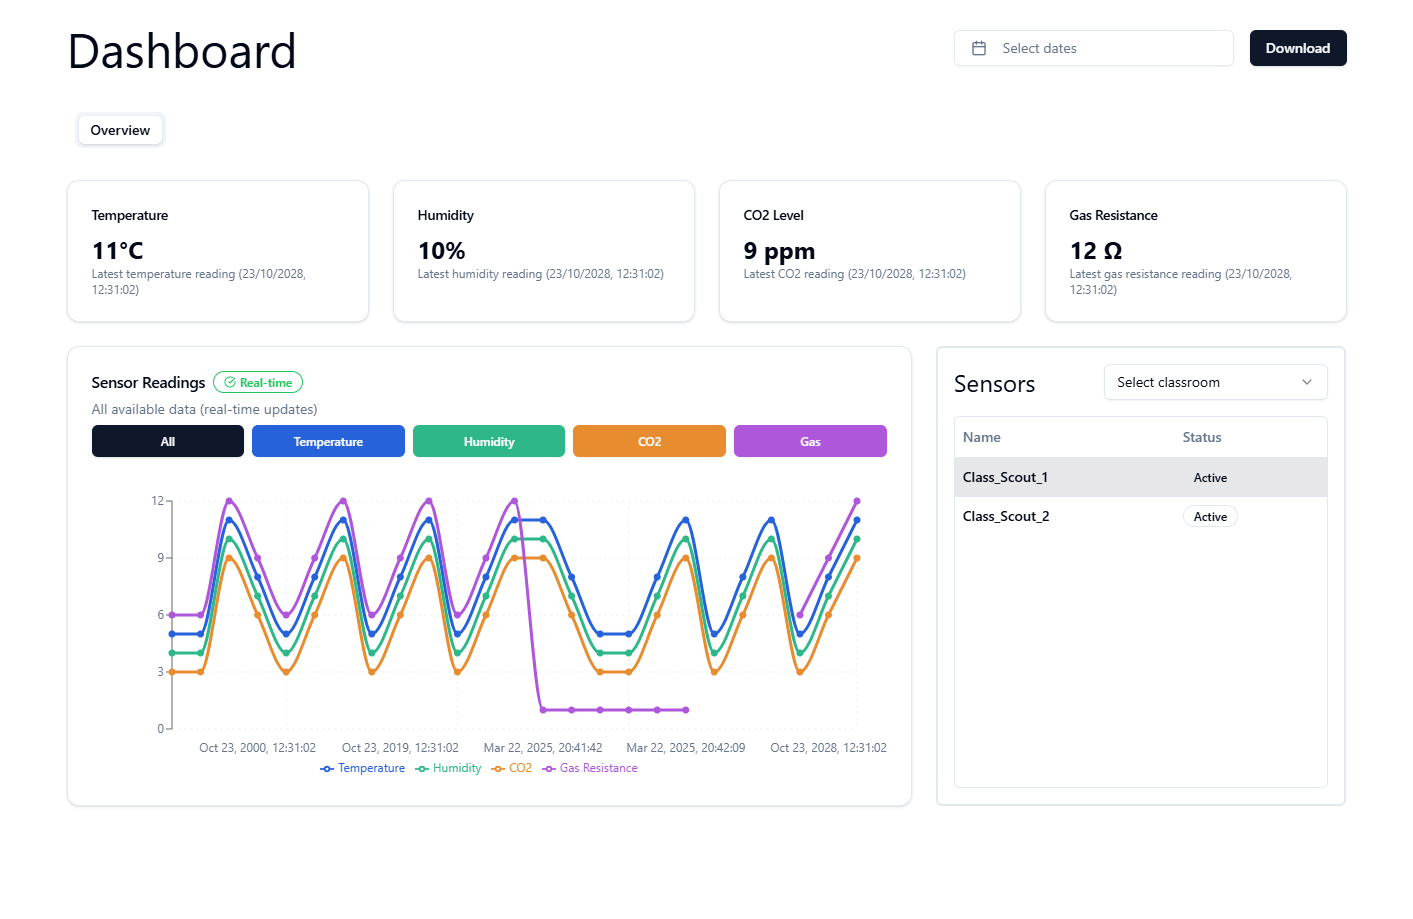
\includegraphics[width=1\textwidth]{files/Thomas/pics/Website/dashbord/dashbaord-screen.png}
\caption[Bildbezeichnung für Abbildungsverzeichnis]{Dashbaord}
\label{fig:gehaeuse_internet_bild}
\end{figure}

\subsection{DatePicke}

\begin{figure}[!htb]
\centering
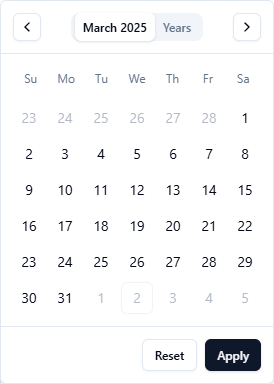
\includegraphics[width=1\textwidth]{files/Thomas/pics/Website/dashbord/dashbaord-datepicker.png}
\caption[Bildbezeichnung für Abbildungsverzeichnis]{flowchart of datepicker}
\label{fig:gehaeuse_internet_bild}
\end{figure}


Für das auswählen das man in einen gewissen Zeitraum die Daten auswählen kann wurde ein DatePicker Komponente erstellt die einen gewissen zeitraum einstellen kann


\begin{figure}[!htb]
\centering
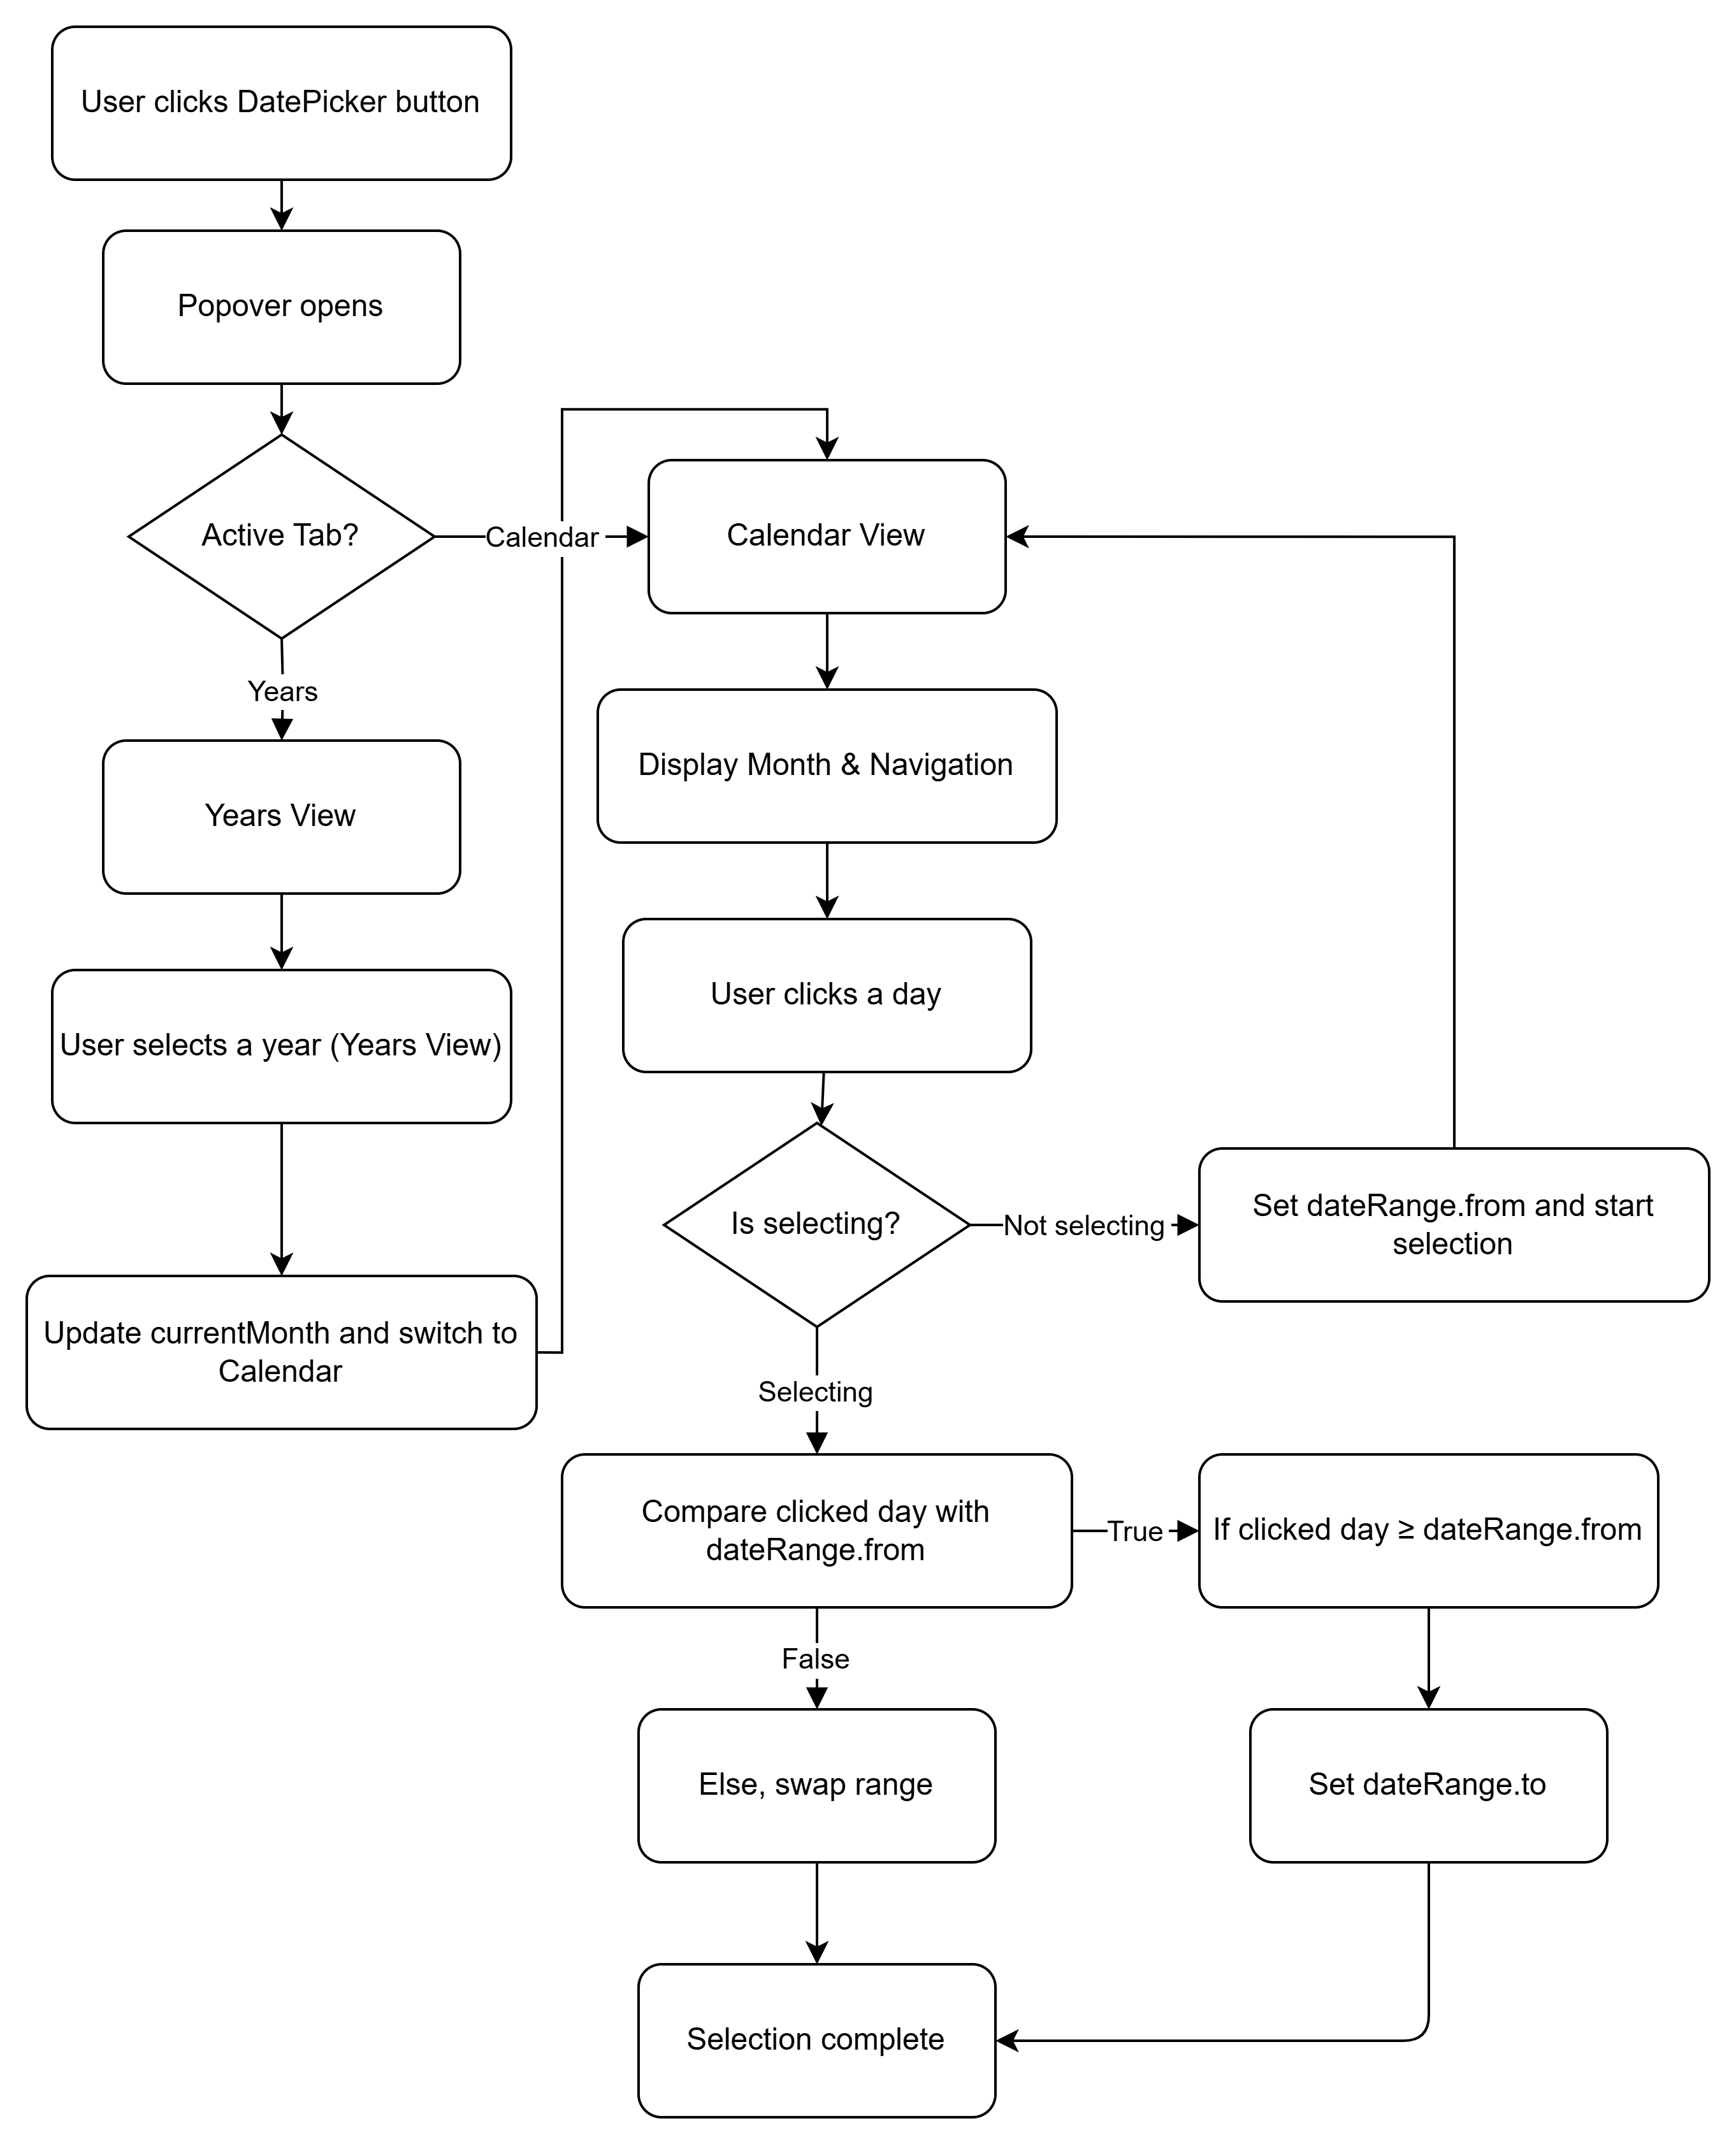
\includegraphics[width=1\textwidth]{files/Thomas/pics/Website/dashbord/dashbaord-datepicker-flowchart.png}
\caption[Bildbezeichnung für Abbildungsverzeichnis]{flowchart of datepicker}
\label{fig:gehaeuse_internet_bild}
\end{figure}


\clearpage

\subsection{Diagramm}

\begin{figure}[!htb]
\centering
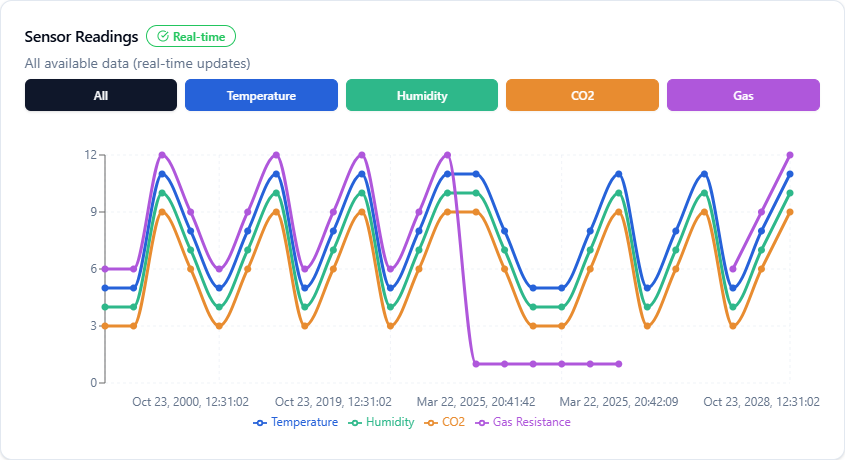
\includegraphics[width=1\textwidth]{files/Thomas/pics/Website/dashbord/chart.png}
\caption[Bildbezeichnung für Abbildungsverzeichnis]{Diagramm Dashboard}
\label{fig:Flowchart_Backend}
\end{figure}

Das Diagramm wrude mit den Diagrammen von Shadcn gemacht. Die Werte die angezeigt werden sollten sind.

\begin{itemize}
    \item Temperature

    \item Humidity

    \item CO2

    \item Gas Resistance
\end{itemize}

\begin{figure}[!htb]
\centering
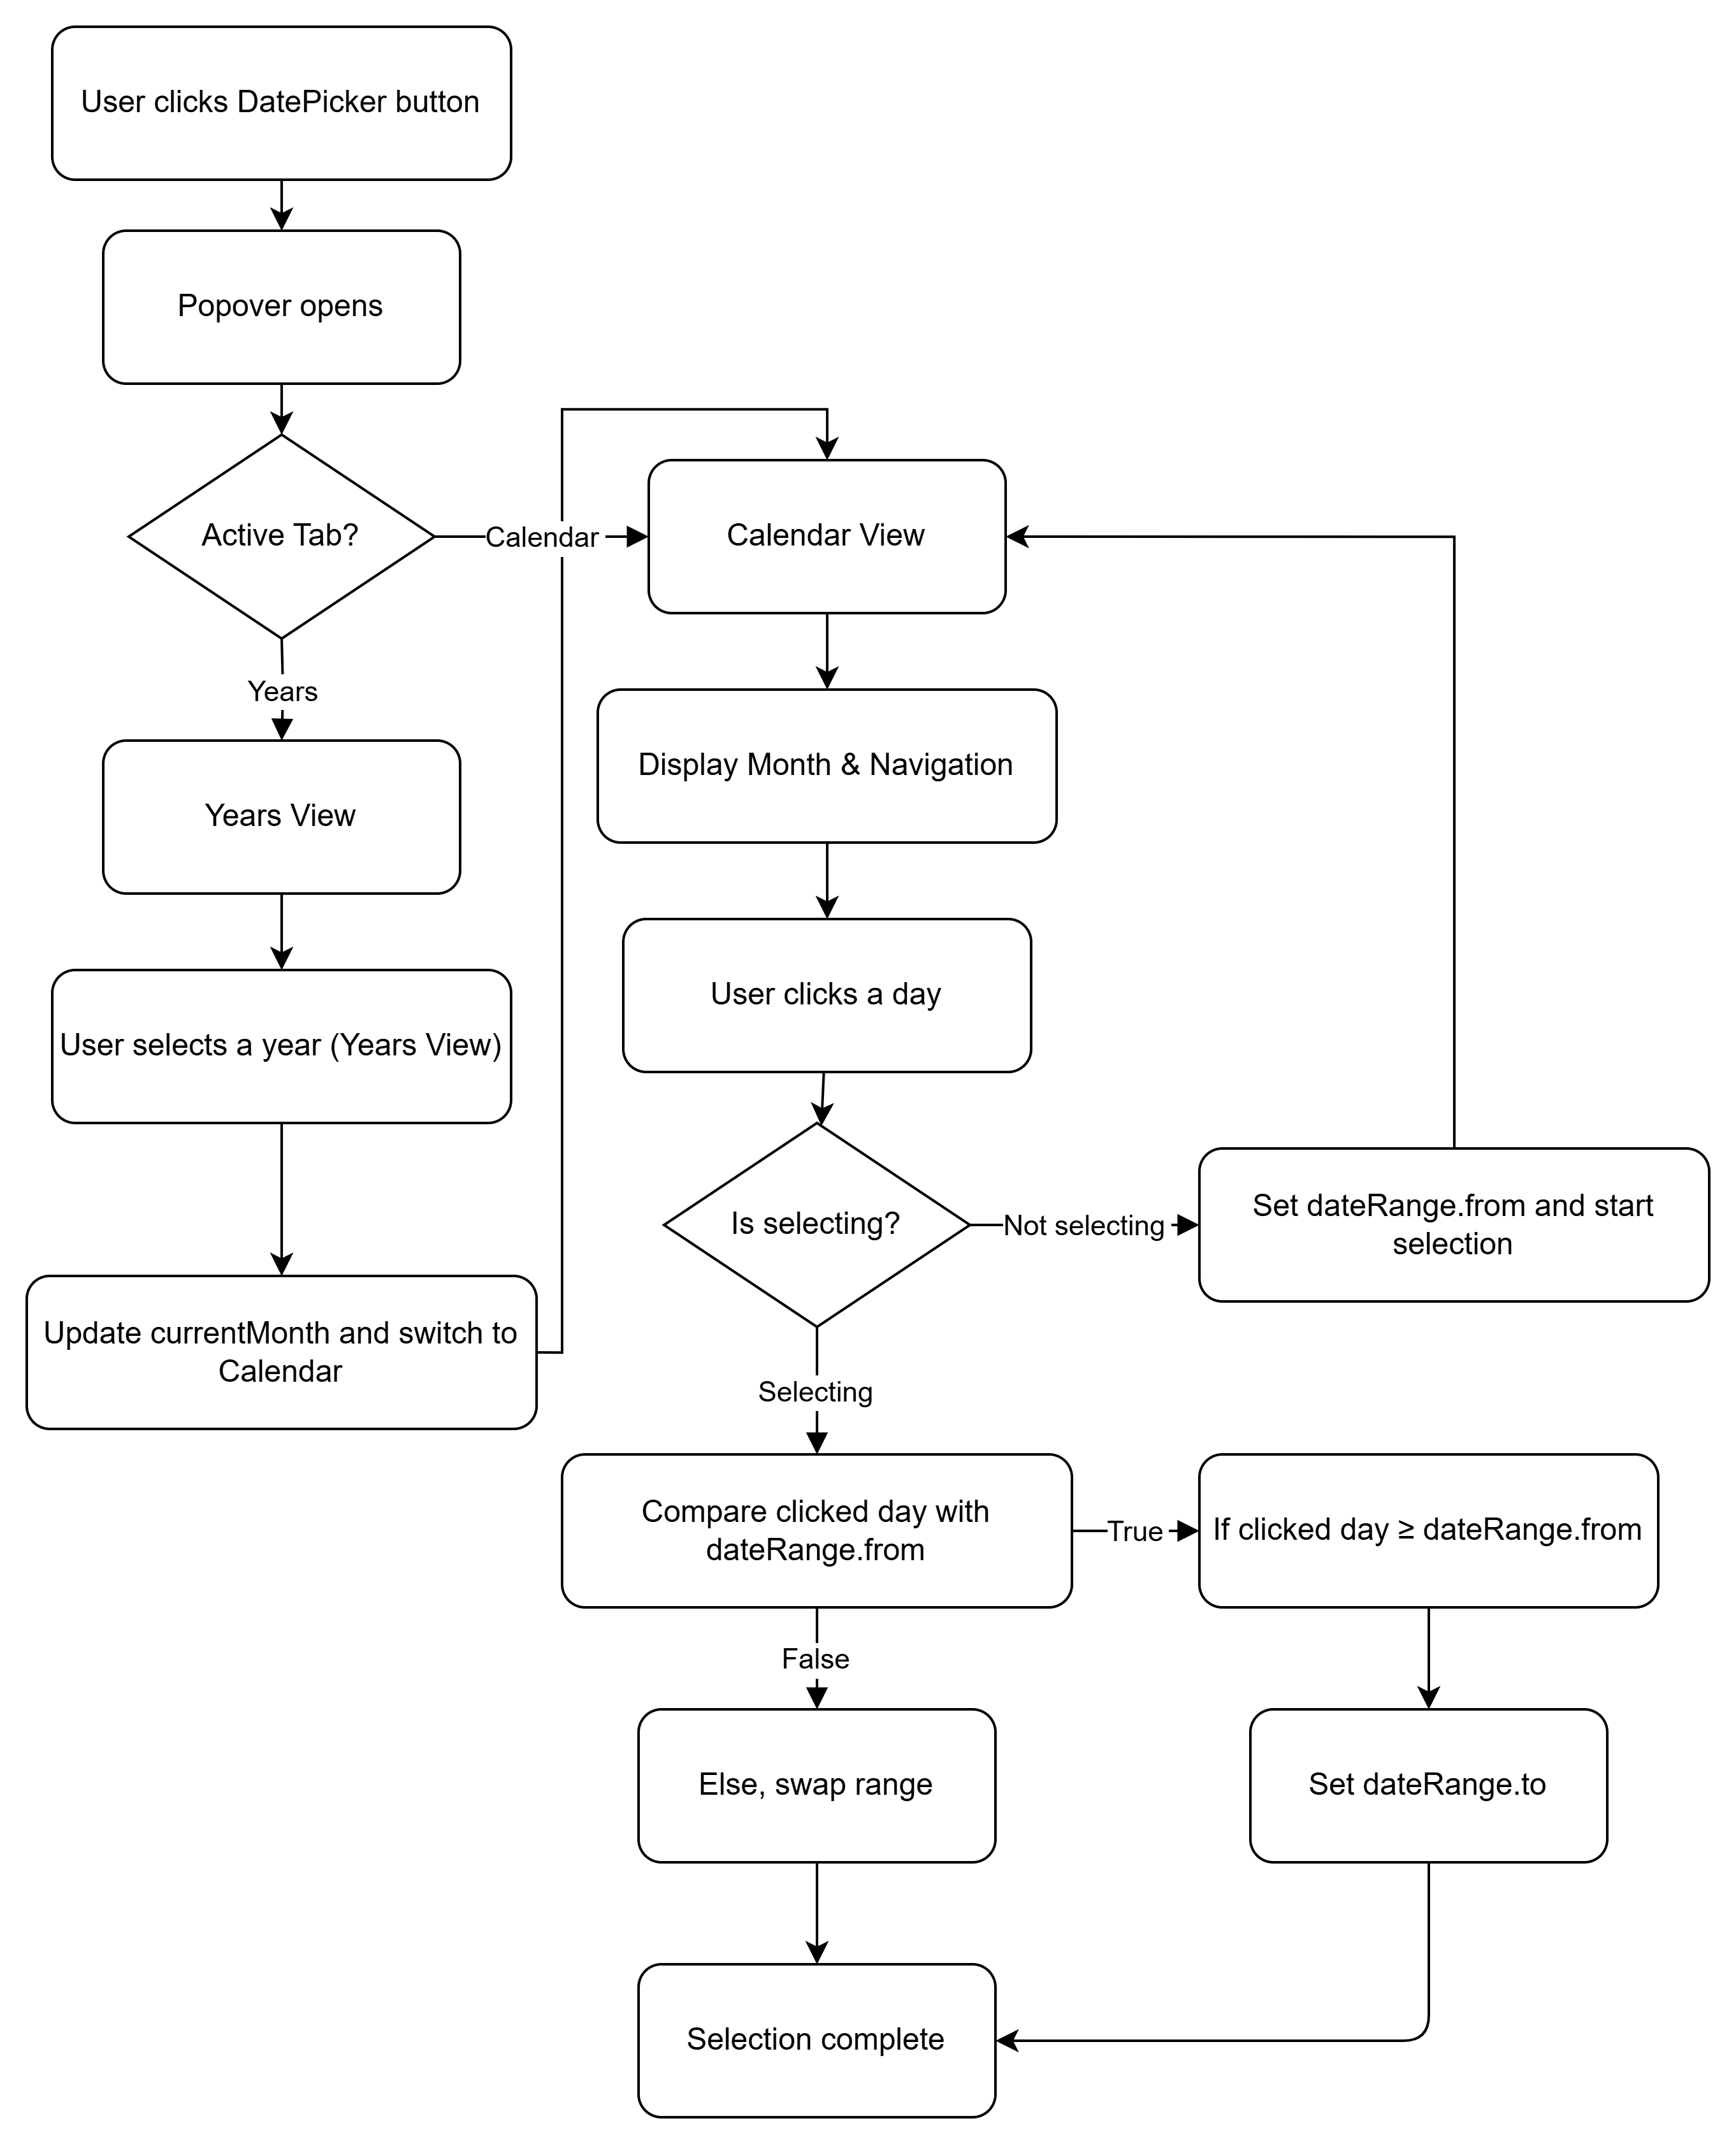
\includegraphics[width=1\textwidth]{files/Thomas/pics/Website/dashbord/dashbaord-datepicker-flowchart.png}
\caption[Bildbezeichnung für Abbildungsverzeichnis]{flowchart of chart}
\label{fig:gehaeuse_internet_bild}
\end{figure}

Da nicht jederzeit alle Werte gleichzeitig angezeigt werden sollen, wurde eine Lösung mit Schaltflächen implementiert, um einzelne Linien flexibel ein- oder auszublenden.
Mithilfe von \texttt{zustand} wird im folgenden Code-Snippet im State gespeichert, welche Linien aktuell sichtbar sind.

Zunächst wird geprüft, ob die Schaltfläche \texttt{"all"} gedrückt wurde. In diesem Fall werden entweder alle vier Linien gleichzeitig ein- oder ausgeblendet, je nachdem, ob aktuell bereits alle sichtbar sind.
Wird hingegen eine einzelne Linie ein- oder ausgeblendet, so wird ihr Name entweder aus dem \texttt{activeLines}-Array entfernt oder wieder hinzugefügt.

\begin{lstlisting}[language=mytsx]
toggleLine: (line) => {
    const { activeLines } = get();
    
    if (line === "all") {
      // Alle Linien ein-/ausblenden
      if (activeLines.length === 4) {
        set({ activeLines: [] });
      } else {
        set({ activeLines: ["temperature", "humidity", "co2", "gas_resistance"] });
      }
    } else {
      // Einzelne Linie ein-/ausblenden
      if (activeLines.includes(line)) {
        set({ activeLines: activeLines.filter(l => l !== line) });
      } else {
        set({ activeLines: [...activeLines, line] });
      }
    }
  },
\end{lstlisting}







\subsection{Realtime}
\label{ref:realtime-sensor}

Im folgenden Code-Snippet wird eine Realtime-Subscription für einen Sensor eingerichtet.  
Dabei wird ein Channel auf der Tabelle \texttt{sensor\_readings} erstellt, der jedes Mal einen Callback auslöst, sobald sich über \texttt{postgres\_changes} eine Änderung für genau diesen Sensor ereignet.

\begin{lstlisting}[language=mytsx]
export async function subscribe_to_sensor_readings(
  callback: (payload: RealtimePostgresChangesPayload<SensorReadingRow>) => void,
  sensorId: string
): Promise<RealtimeChannel> {
  const supabase = await createClient();
  const channel = supabase
    .channel(`sensor-readings-${sensorId}`)
    .on(
      'postgres_changes',
      {
        event: '*',
        schema: 'public',
        table: 'sensor_readings',
        filter: `sensor_id=eq.${sensorId}`,
      },
      (payload) => callback(payload as RealtimePostgresChangesPayload<SensorReadingRow>)
    )
    .subscribe();
  
  return channel;
}
\end{lstlisting}


\newpage


\subsection{Cards}

Auf dem Dashboard werden 4 Karten angezeit wo jede den aktulesten wert anzeigt der von dem Sensor gemessen wurde. Dies wurde auch mittels der gelichen Reatlime \ref{ref:realtime-sensor} implementiert.


\begin{figure}[!htb]
\centering
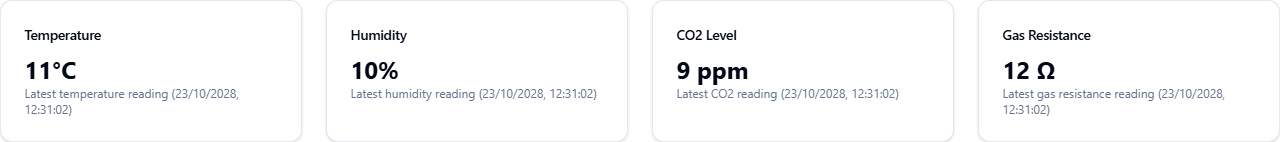
\includegraphics[width=1\textwidth]{files/Thomas/pics/Website/dashbord/dashboard-card.png}
\caption[Bildbezeichnung für Abbildungsverzeichnis]{flowchart of chart}
\label{fig:gehaeuse_internet_bild}
\end{figure}




\newpage

Im zweiten Code-Snippet wird der Channel mithilfe von \texttt{zustand} im State gespeichert.  
Zusätzlich wird hier festgelegt, dass der Callback nur bei einem \texttt{INSERT} oder \texttt{UPDATE} ausgelöst wird.  
Bei einer solchen Änderung wird ein neues Sensor-Reading zur State-Variable hinzugefügt.

\begin{lstlisting}[language=mytsx]
subscribeToReadings: async (sensorId) => {
    try {
      const channel = await subscribe_to_sensor_readings(
        (payload) => {
          console.log('Real-time sensor reading received:', payload);
          
          if (payload.eventType === 'INSERT' || payload.eventType === 'UPDATE') {
            const newReading = payload.new as SensorReadingRow;
            get().addReading(newReading);
          }
        },
        sensorId
      );
      
      set({ realtimeSubscriptions: { ...get().realtimeSubscriptions, readings: channel } });
    } catch (error) {
      console.error('Error setting up real-time subscription:', error);
    }
  },
\end{lstlisting}






\newpage

\section{Backend}

Das Backend kann auf /api/sensor-data mittels einen Post request daten geschickt werden wie in \ref{ref:backend_design} beschreiben. Wie diese Daten verarbeitet werden kann man im flowchart \ref{fig:Flowchart_Backend} sehen.

\begin{figure}[!htb]
\centering
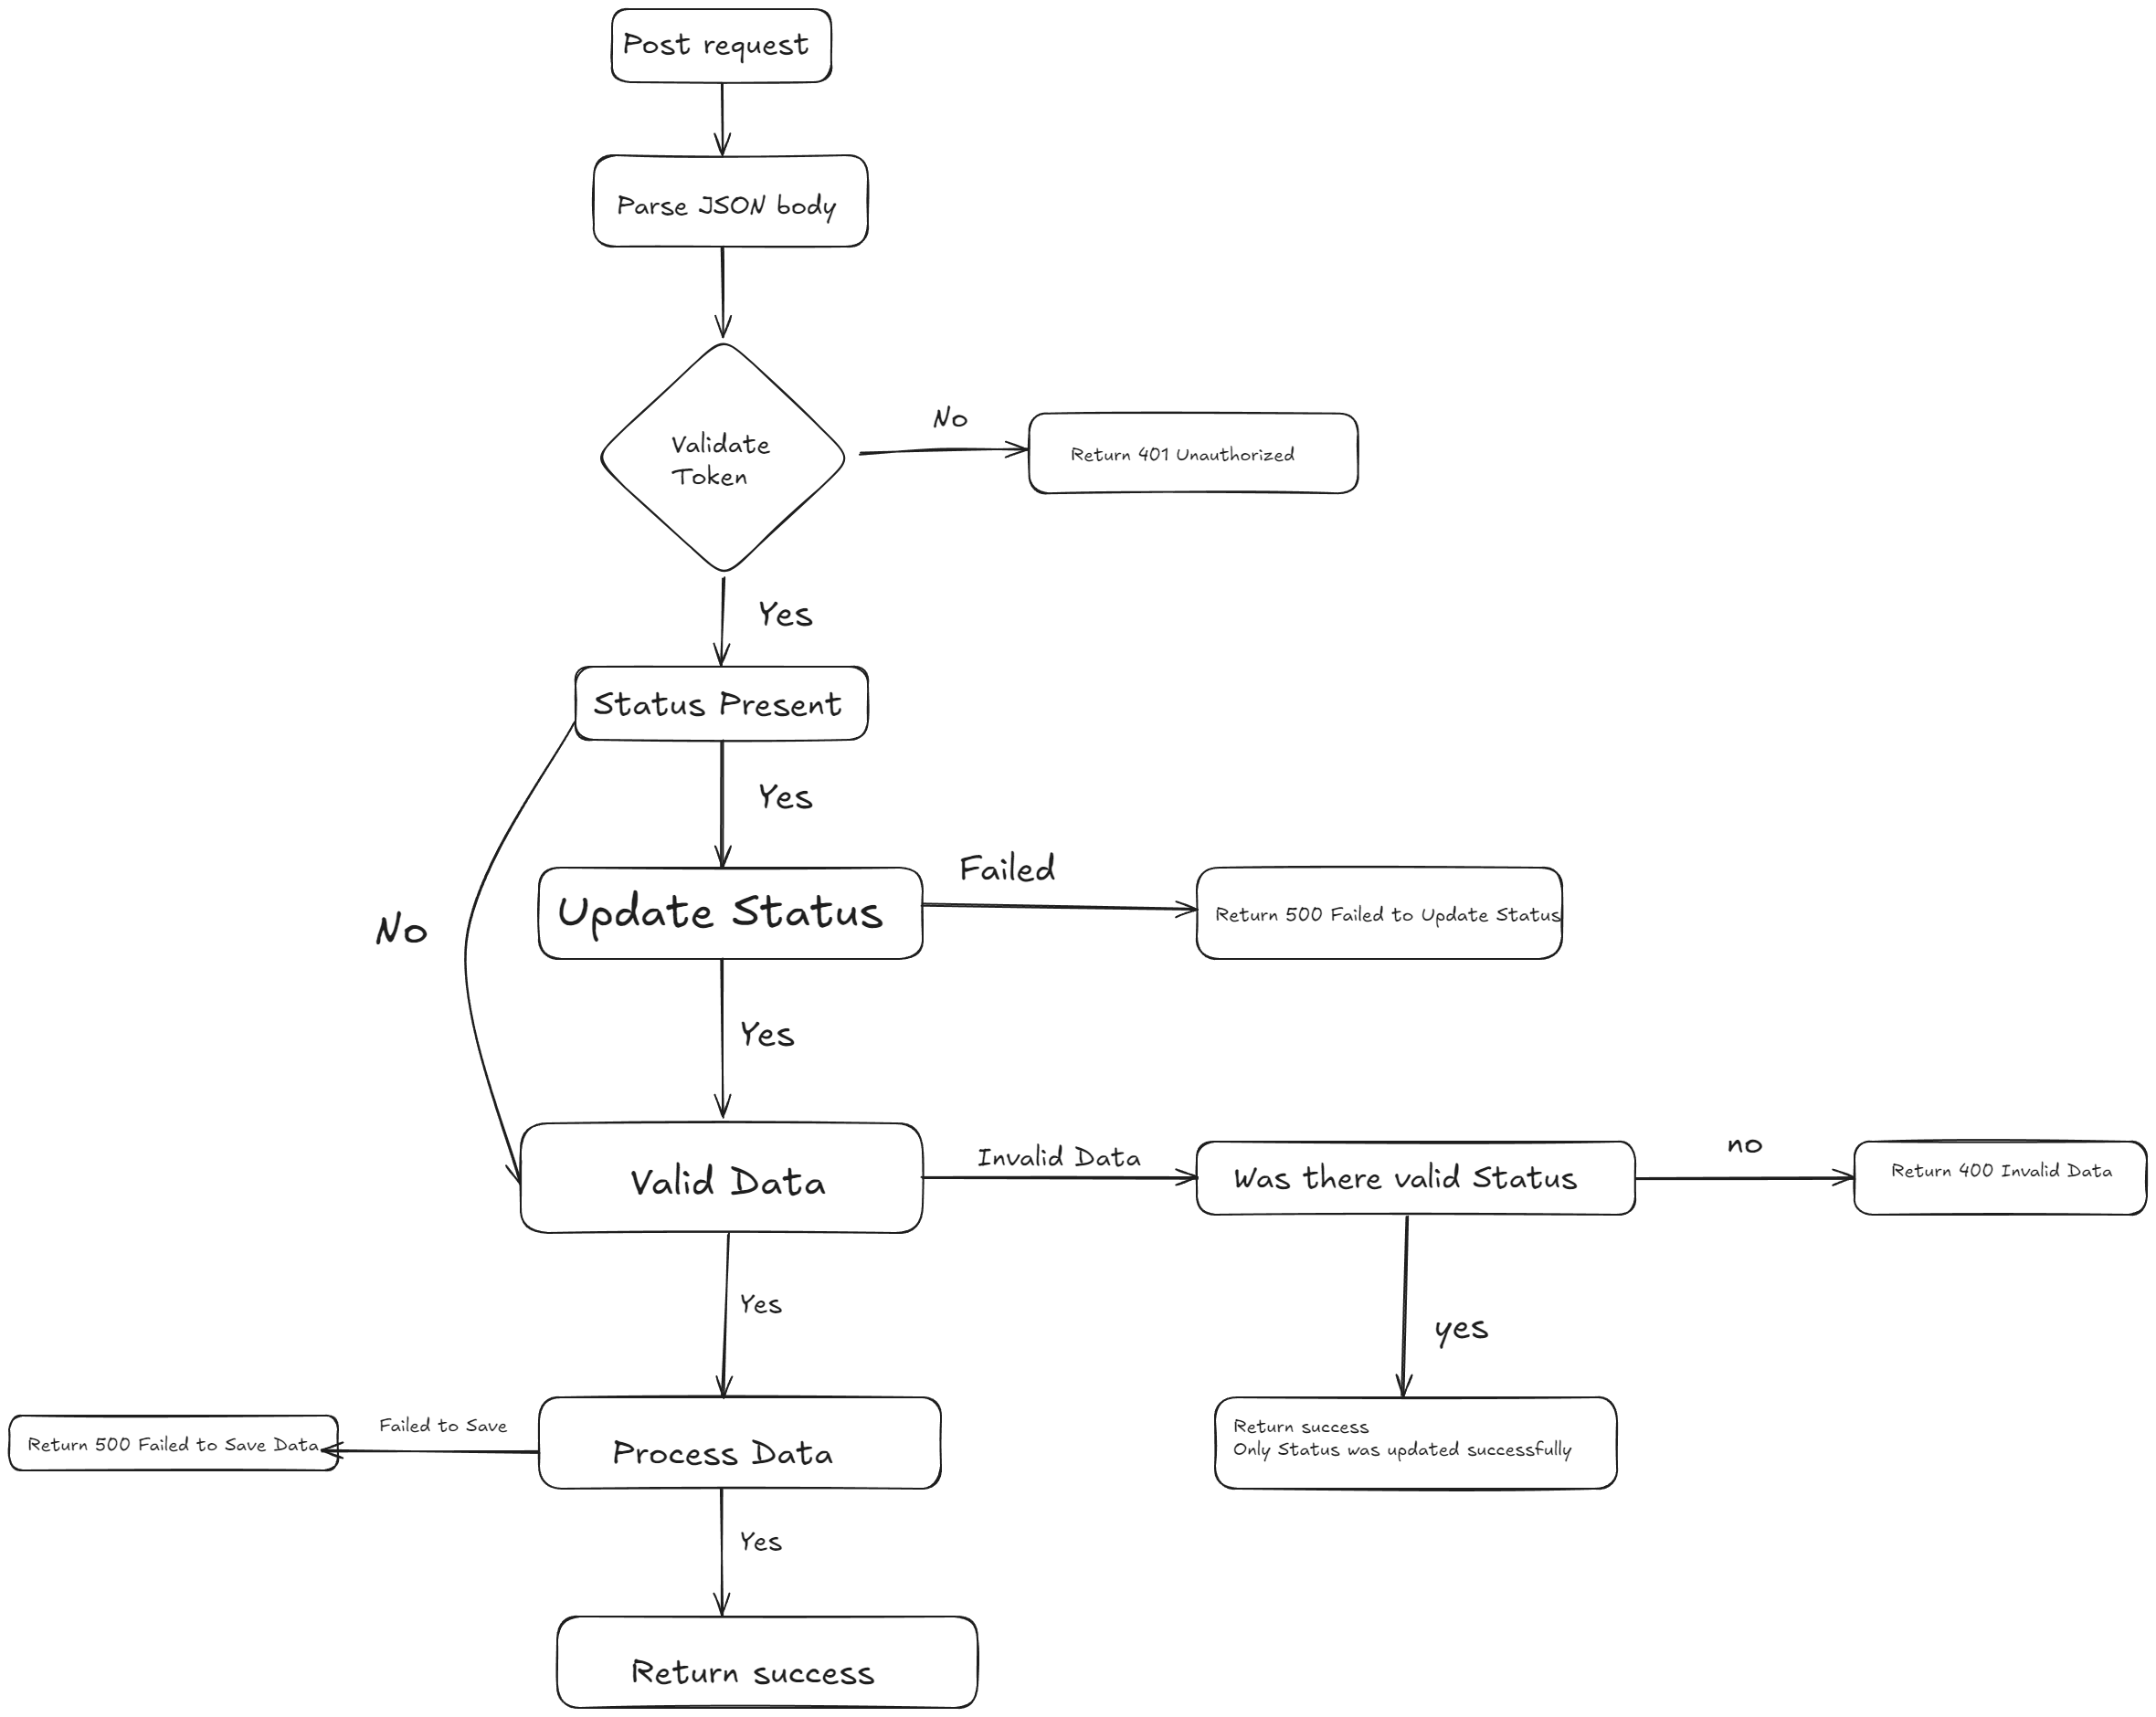
\includegraphics[width=1\textwidth]{files/Thomas/pics/Website/backend/image.png}
\caption[Bildbezeichnung für Abbildungsverzeichnis]{Flowchart vom Backend}
\label{fig:Flowchart_Backend}
\end{figure}

Durch diesen Abluaf wird sicher gestellt das die Daten Valide sind.

\newpage

In diesen Code Snipet wird geprüft ob der token(uuid des Sensors) Valide ist und wenn nicht wird ein error zurückgeschickt mit dem Statuts 401 und einen Text Unauthorized

\begin{lstlisting}[language=mytsx]
const isValidToken = await validate_sensor_token(token);
        
        if (!isValidToken) {
            return NextResponse.json({ error: 'Unauthorized' }, { status: 401 });
        }
\end{lstlisting}

\vspace{1cm}

In diesen Code am schluss der route wird geprüft ob die sensor daten in die Datenbank gespeichert werden konnten. Wenn dies nicht der Fall ist wird ein Error zürckgeschickt mit dem Status 500 und der Nachricht Failed to save data


\begin{lstlisting}[language=mytsx]
const { success, error } = await insert_sensor_readings(validReadings);

            if (!success) {
                console.error('Error inserting data:', error);
                return NextResponse.json({ error: 'Failed to save data' }, { status: 500 });
            }
\end{lstlisting}




\clearpage





\end{inhalt}     

%Chapter 9 Gehäuse
\responsible{Thomas Potzmader} 
\begin{inhalt}
\renewcommand*\chapterpagestyle{scrheadings}
\chapter{Gehäuse}

Für das Gehäuse wurde, wie in \ref{ref:fusion360_grundlagen} beschrieben, \texttt{Fusion 360} verwendet, um ein passendes Design zu erstellen.  
Um ein präzises Gehäuse zu konstruieren, sind einige vorbereitende Schritte notwendig.  
In diesem Fall wurde die Leiterplatte (PCB) aus \texttt{Altium Designer} als \texttt{STEP}-Datei exportiert und anschließend in \texttt{Fusion 360} importiert,  
um ein passgenaues Gehäuse um die Platine herum modellieren zu können.  
Hierfür wurde ein spezifischer Leitfaden verwendet \cite{artikel_pcb_way}.


\begin{figure}[!htb]
\centering
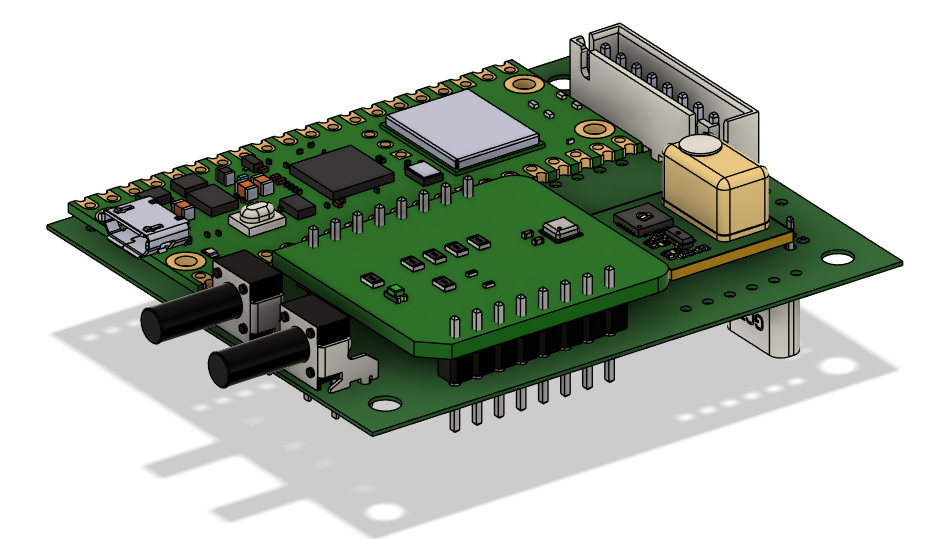
\includegraphics[width=0.65\textwidth]{files/Thomas/pics/geheause/pcb_fusion.png}
\caption[3D Model PCB V2.0]{3D Model PCB V2.0}
\label{fig:pcb_v2}
\end{figure}


Außerdem wurde das Displaymodell von einer Website \cite{3d_display_website} heruntergeladen und in das Projekt integriert.


\begin{figure}[!htb]
\centering
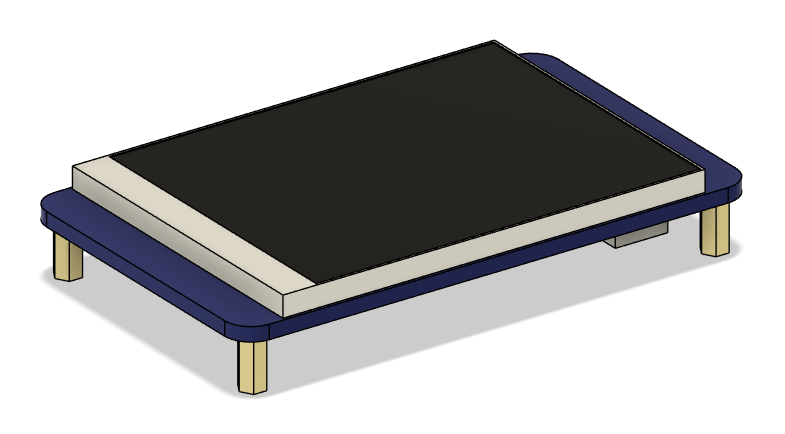
\includegraphics[width=0.55\textwidth]{files/Thomas/pics/geheause/display_fusion.png}
\caption[3D Model Display]{3D Model Display}
\label{fig:display_3d}
\end{figure}

\clearpage

\section{Version 1.0}
\label{ref:gehaeuse_1_0}

\begin{figure}[!htb]
\centering
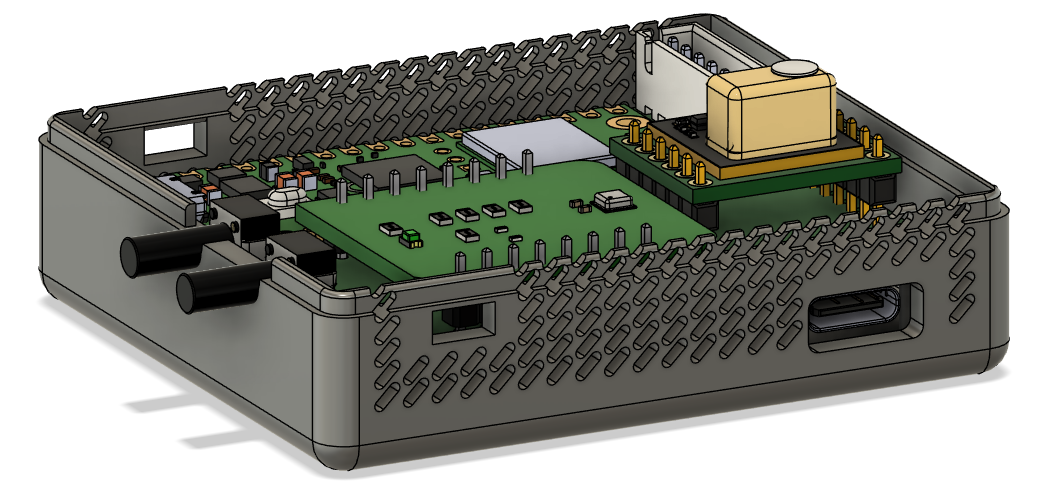
\includegraphics[width=0.45\textwidth]{files/Thomas/pics/geheause/1.0/gehaeuse_side.png}
\caption[Gehäuse V1.0 von der Seite]{Gehäuse V1.0 von der Seite}
\label{fig:gehaeuse_side_v1_0}
\end{figure}

Beim ersten Meilenstein traten noch zahlreiche Probleme auf. Wie in der Abbildung \ref{fig:gehaeuse_side_v1_0} ersichtlich, basierte diese Version auf der \texttt{PCB} Version 1.0 (\ref{ref:PCB_Version_1}).  
Besonders problematisch war der USB-C-Port an der Seite der Platine. Da dieser sehr nah am Rand der \texttt{PCB} positioniert war und USB-C-Kabel nicht genormte Gehäusegrößen besitzen,  
musste ein besonders großes Loch in das Gehäuse eingeplant werden, um mit allen Steckern kompatibel zu sein.  

\vspace{0.15cm}

Außerdem wurden in der Front nur zwei Clips verwendet, was sich jedoch als unzureichend herausstellte.  


\vspace{0.15cm}

Für einen optimierten Airflow wurde dasselbe Lüftungsmuster verwendet, das zuvor durch Internetrecherche \ref{fig:gehaeuse_internet_bild} identifiziert wurde.



\begin{figure}[!htb]
\centering
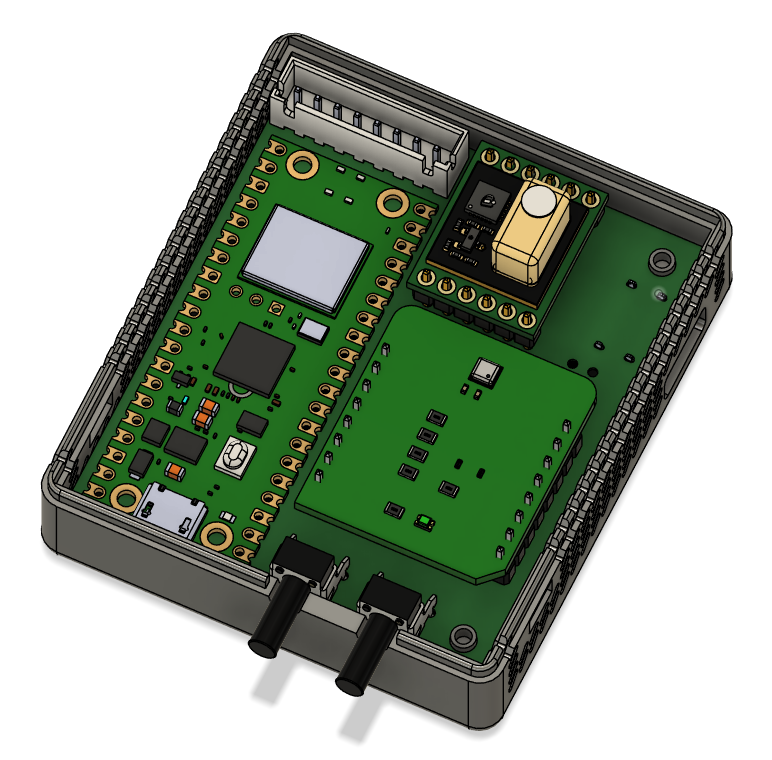
\includegraphics[width=0.4\textwidth]{files/Thomas/pics/geheause/1.0/gehaeuse_top.png}
\caption[Gehäuse V1.0 von Oben]{Gehäuse V1.0 von Oben}
\label{fig:gehaeuse_top_1_0}
\end{figure}


Wie in Abbildung \ref{fig:gehaeuse_top_1_0} zu erkennen ist, waren bei der ersten Version die Wandstärken des Gehäuses sehr gering, wodurch die dünneren Bereiche bei jeder Belastung leicht abbrachen.



\vspace{0.15cm}

Außerdem passte das Display im oberen Teil des Gehäuses noch nicht vollständig.

\newpage

\section{Version 1.1}

\begin{figure}[!htb]
\centering
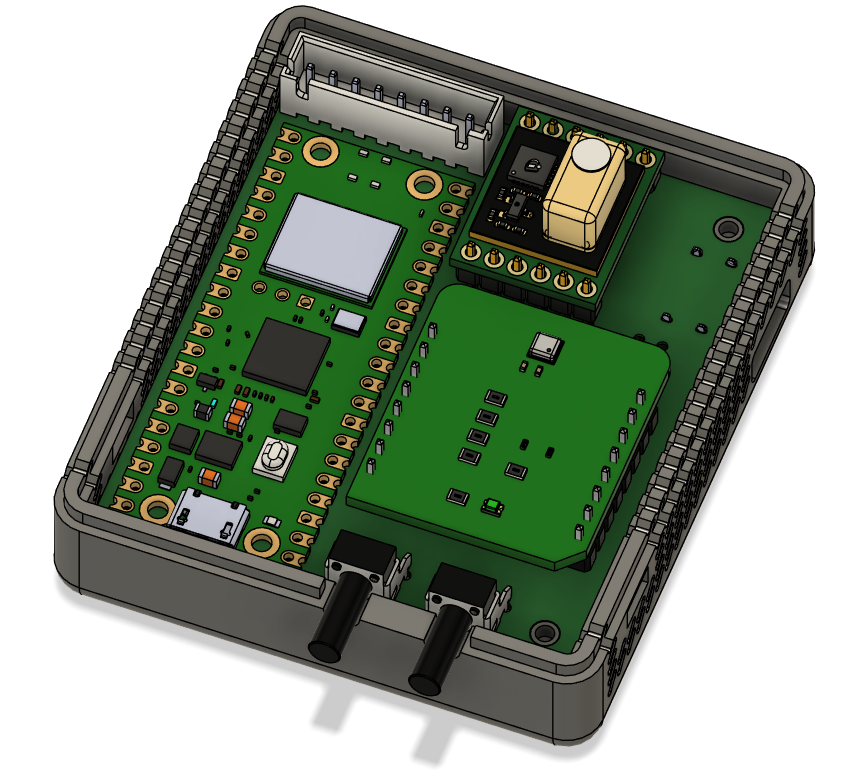
\includegraphics[width=0.55\textwidth]{files/Thomas/pics/geheause/1.1/gehaeuse_top.png}
\caption[Gehäuse V1.1 von Oben]{Gehäuse V1.1 von Oben}
\label{fig:gehaeuse_internet_bild}
\end{figure}

Der wesentliche Unterschied zwischen Version 1.0 (Zu sehen in: \ref{ref:gehaeuse_1_0}) und 1.1 besteht darin, dass die Seitenwände des Gehäuses verstärkt wurden, um eine höhere Stabilität zu gewährleisten und ein leichtes Brechen zu verhindern.

\newpage

\section{Version 1.2}

\begin{figure}[!htb]
\centering
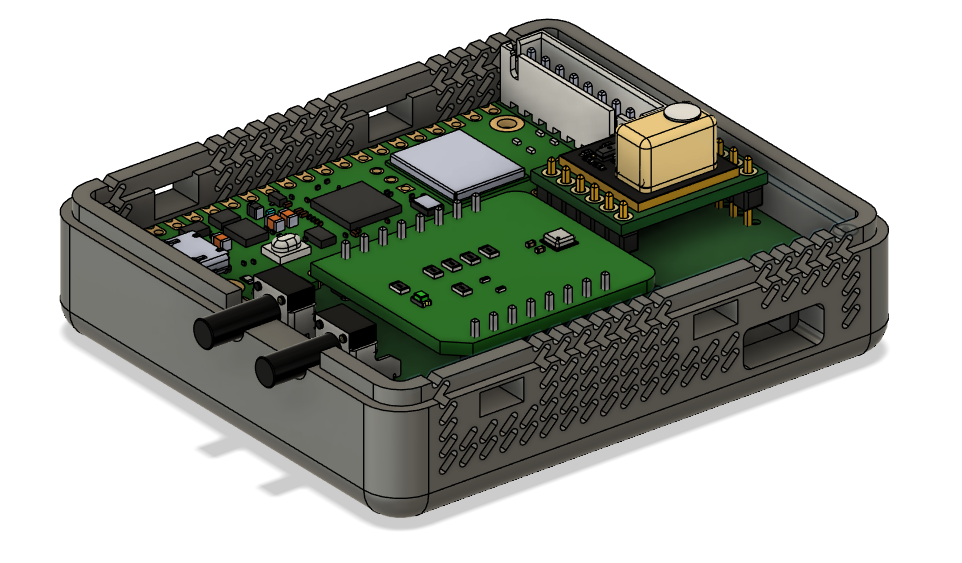
\includegraphics[width=0.6\textwidth]{files/Thomas/pics/geheause/1.2/gehaeuse_side.png}
\caption[Gehäuse V1.2 von der Seit]{Gehäuse V1.2 von der Seite}
\label{fig:gehaeuse_internet_bild}
\end{figure}

In dieser Version wurden zwei zusätzliche Clips hinzugefügt, um den Verschlussmechanismus zu verbessern.  
Ohne diese Ergänzung hätte sich das Gehäuse zu leicht öffnen lassen.

\vspace{1cm}

\begin{figure}[!htb]
\centering
\includegraphics[width=0.6\textwidth]{files/Thomas/pics/geheause/1.2/gehaeuse_back.png}
\caption[Gehäuse V1.2 von Hinten]{Gehäuse V1.2 von Hinten}
\label{fig:gehaeuse_internet_bild}
\end{figure}

Außerdem wurde nun wenn das gehäuse zu stereng aufgeht ein Schlitz zwischen den Obrigen teil und den untrigen Teil gemacht um zu garantiren das man mit einen Schlitzschraufenziher das gehäuse aufzuamachen können.

\vspace{0.15cm}

Zudem wurde die Aussparung für das Display optimiert, sodass es nun passgenau mit den erforderlichen Toleranzen und allen notwendigen Anpassungen in das Gehäuse eingesetzt werden kann.

\newpage

\section{Version 2.0}

\begin{figure}[!htb]
\centering
\includegraphics[width=0.6\textwidth]{files/Thomas/pics/geheause/2.0/gehaeuse_side.png}
\caption[Gehäuse V2.0 von der Seite]{Gehäuse V2.0 von der Seite}
\label{fig:gehaeuse_internet_bild}
\end{figure}

Nachdem die \texttt{PCB} Version 2 (Siehe auf: \ref{ref:PCB_Version_2}) fertiggestellt war, wurde das Gehäuse neu designt, um erneut zur Platine zu passen.  
Ein wesentlicher Vorteil dieser Version besteht darin, dass sich der USB-C-Anschluss nicht mehr seitlich befindet.  
Dadurch konnten die Clips symmetrisch und in gleichem Abstand zur Gehäusemitte positioniert werden, was eine deutlich stabilere Verbindung zwischen den Gehäuseteilen ermöglicht.
 

\vspace{0.15cm}

Zusätzlich wurden kleine Schlitze in das Gehäuse integriert, um die Montage im Kabelkanal der Schulräume der HTL St. Pölten zu erleichtern.  
Diese Schlitze ermöglichen es, das Gerät einfach in den dafür vorgesehenen Adapter einzustecken.


\begin{figure}[!htb]
\centering
\includegraphics[width=0.5\textwidth]{files/Thomas/pics/geheause/2.0/gehaeuse_bot.png}
\caption[Gehäuse V2.0 von Unten]{Gehäuse V2.0 von Unten}
\label{fig:gehaeuse_internet_bild}
\end{figure}

Da sich der USB-C-Anschluss nun nicht mehr an der Seite, sondern an der Unterseite des Gehäuses befindet, entfällt das Problem unterschiedlicher USB-C-Steckergrößen.  
Somit ist gewährleistet, dass sämtliche USB-C-Kabel problemlos passen.


\section{Version 2.1}

\begin{figure}[!htb]
\centering
\includegraphics[width=0.65\textwidth]{files/Thomas/pics/geheause/2.1/gehaeuse_side.png}
\caption[Obrige Gehäuseteil V2.1 von Unten]{Obrige Gehäuseteil V2.1 von Unten}
\label{fig:gehaeuse_internet_bild}
\end{figure}



Da die Clips wiederholt Probleme verursachten, wurden sie im Inneren verstärkt.  
Zudem wurden sie verkleinert, um Konflikte mit der Gehäusedicke zu vermeiden.


\newpage

\section{Adapter für Kabelkanal}

Für die Installation des ClassScouts in den Klassenräumen wurde ein spezieller Adapter entworfen, der dafür vorgesehen ist, im Kabelkanal der HTL St. Pölten montiert zu werden.


\subsection{Version 1.0}

In der ersten Version wurde probiert einfach die Mase des Kabelkanals zu Treffen und zu schauen das die Knöpfe drückbar sind von außen.

\begin{figure}[!htb]
\centering
\includegraphics[width=0.5\textwidth]{files/Thomas/pics/adapter/1.0/image.png}
\caption[Gehäuse Adapter V1.0]{Gehäuse Adapter V1.0}
\label{fig:gehaeuse_internet_bild}
\end{figure}


\subsection{Version 2.0}

In Version 2 wurde eine Öffnung für ein USB-C-Kabel hinzugefügt, sodass dieses nun von außen in den Kabelkanal geführt werden kann.  
Zudem wurden die Toleranzen optimiert, um den Einbau des Gehäuses zu erleichtern.


\begin{figure}[!htb]
\centering
\includegraphics[width=0.55\textwidth]{files/Thomas/pics/adapter/2.0/image.png}
\caption[Gehäuse Adapter V2.0]{Gehäuse Adapter V2.0}
\label{fig:gehaeuse_internet_bild}
\end{figure}



\section{Slicen und 3D-Druck}

Da bei einem FDM-3D-Drucker Schicht für Schicht aufgebaut wird, entstehen leicht geradlinige Bruchstellen.  
Besonders problematisch war dies bei den Clips, die das Gehäuse zusammenhalten sollten.  
Nach längerem Ausprobieren wies ein Klassenkollege darauf hin, dass sich das Problem durch das Drucken des Gehäuses in einem Winkel von 45° lösen ließe.  
Durch diese Ausrichtung verlaufen die Schichten schräg, wodurch sie sich nicht so leicht voneinander trennen und die Clips deutlich stabiler werden.  
Diese Methode wurde umgesetzt und das Problem erfolgreich behoben.


\begin{figure}[!htb]
\centering
\includegraphics[width=0.75\textwidth]{files/Thomas/pics/geheause/gehaeuese_45_Grad_druck.png}
\caption[Gehäuse 45° Druck]{Gehäuse 45° Druck}
\label{fig:gehaeuse_internet_bild}
\end{figure}

Das Gehäuse wurde mit einem \texttt{Bambu Lab A1} FDM-3D-Drucker gefertigt und zuvor mit dem \texttt{Bambu Slicer} gesliced, um einen optimalen G-Code zu generieren.  
Die Clips wurden mit einer Füllung von 100\% gedruckt, während der restliche Teil des Gehäuses mit einer Füllung von 20\% gedruckt wurde.  
Zudem musste das Gehäuse mit einer Schichthöhe von 0{,}1\,mm gedruckt werden, um das Lüftungsmuster korrekt zu drucken.


\end{inhalt}   


%%ANHANG
\begin{inhalt}
\renewcommand*\chapterpagestyle{scrheadings}
\chapter{Ergebnisse \& Ausblick}

Die in Kapitel \ref{sec:PCBVersion2} entwickelte Platine konnte erfolgreich entworfen und bestückt werden (Abb. \ref{fig:fertigeplatine}). Sie wurde erfolgreich auf ihre Funktionalität getestet.

\bigskip \\

Der Mikrocontroller liest die Messdaten der Sensoren erfolgreich aus und gibt sie auf dem Display aus (Abb. \ref{fig:fertigesGerat}). Das Display besitzt, wie in Kapitel \ref{sec:display interface} beschrieben, drei verschiedene Seiten, zwischen denen gewechselt werden kann. Die Taster erfüllen dabei ihre Funktionen (Kapitel \ref{sec:BeutzerInteraktionen}). Die Datenübertragung an den Webserver über HTTPS, sowie die Skala am Display, ist mit Stand vom 02.04.2025 aufgrund von Zeitknappheit noch nicht funktionstüchtig.


\begin{figure}[!htb]
    \centering
    \begin{subfigure}[b]{0.49\textwidth}
        \includegraphics[width=\textwidth]{files/Tobias/pics/Platine (2).jpg}
        \caption{Fertiggestellte Platine}
        \label{fig:fertigeplatine}
    \end{subfigure}
    \hfill
    \begin{subfigure}[b]{0.49\textwidth}
        \includegraphics[width=\textwidth]{files/Tobias/pics/Geraet.jpg}
        \caption{Fertiggestelltes Messgerät}
        \label{fig:fertigesGerat}
    \end{subfigure}
    \caption[Hardware \& Mikocontrollerprogrammierung - Ergebnisse]{Hardware \& Mikocontrollerprogrammierung - Ergebnisse}
    \label{fig:Ergebnisse}
\end{figure}


Die ursprünglich geplante App wurde verworfen, da sich nach intensiver Recherche \cite{youtube_no_app} herausstellte, dass sich die Software besser als Web-Anwendung anstatt als mobile Smartphone-App umsetzen lässt.  
Aus diesem Grund wurden alle zu Beginn erstellten Flutter-Projekte pausiert und stattdessen eine Webseite entwickelt.  
Die in Kapitel \ref{ref:Website} vorgestellte Webseite konnte erfolgreich fertiggestellt werden.  
Zwar sind aktuell noch einige kleinere Bugs vorhanden, diese sollen jedoch in Zukunft behoben werden.  
Die Realtime-Funktionalität, beispielsweise in den Diagrammen, funktioniert bereits zuverlässig.
\vspace{0.1cm}
Das Gehäuse funktioniert einwandfrei, es konnten keine Fehler festgestellt werden und es wurde erfolgreich und zuverlässig getestet.


\begin{figure}[!htb]
    \centering
    \begin{subfigure}[b]{0.49\textwidth}
        \includegraphics[width=\textwidth]{files/Thomas/pics/Website/dashbord/dashbaord-screen.png}
        \caption{Fertiges Dashboard}
        \label{fig:dashboard_fertig}
    \end{subfigure}
    \hfill
    \begin{subfigure}[b]{0.49\textwidth}
        \includegraphics[width=\textwidth]{files/Thomas/pics/image.png}
        \caption{Fertiges Gehäuse in Kabelkanal}
        \label{fig:dashboard_zweites}
    \end{subfigure}
    \caption[Fertige Diplomarbeitsteile]{Fertiges Diplomarbeitsteile}
    \label{fig:dashboard_vergleich}
\end{figure}


Für die weitere Entwicklung wurde erkannt, dass sich das globale State-Management einfacher mit Cookies als über die URL realisieren lässt.  
Hierfür könnten Bibliotheken wie \texttt{zustand} verstärkt zum Einsatz kommen, da \texttt{Next.js} im Gegensatz zu anderen JavaScript-Frameworks kein eingebautes globales State-Management bietet.  
Außerdem wäre es sinnvoll, künftig auch den Status der Sensoren in die Webseite zu integrieren.





\end{inhalt}  
%===================================
\appendix
\responsible{Thomas Potzmader, Tobias Geppl} 

%=============================%%
%Chapter 4 Ergebnisse
                                    %Ergebnisse(LaTeX File) einfügen

%=============================%%

%%Literaturverzeichnis
%=============================%%
%
\begin{thebibliography}{9999}

\section*{Internetlinks}

\bibitem{AltiumDesignerWiki}
\textbf{Altium Designer:} \textit{Was ist Altium Designer}, 18. September 2024.  
\url{https://de.wikipedia.org/wiki/Altium_Designer}

\bibitem{I2CKommunikation}
\textbf{I2C-Bussystem:} \textit{Was ist I2C}, 18. September 2024.  
\url{https://de.wikipedia.org/wiki/I%C2%B2C}

\bibitem{SPI_Kommunikation}
\textbf{SPI-Bussystem:} \textit{Was ist SPI}, 18. September 2024.  
\url{https://de.wikipedia.org/wiki/Serial_Peripheral_Interface}

\bibitem{HTTPS_Kommunikation}
\textbf{HTTPS-Protokoll:} \textit{Was ist HTTPS}, 18. September 2024.  
\url{https://de.wikipedia.org/wiki/Hypertext_Transfer_Protocol_Secure}

\bibitem{VisualStudioCode}
\textbf{Visual Studio Code:} \textit{Editor für Softwareentwicklung}, 18. September 2024.  
\url{https://de.wikipedia.org/wiki/Visual_Studio_Code}

\bibitem{Raspberry_Pi_Pico_Erweiterung}
\textbf{Raspberry Pi Pico – I/O-Erweiterung:} \textit{Technische Beschreibung}, 18. September 2024.  
\url{https://de.wikipedia.org/wiki/Hypertext_Transfer_Protocol_Secure}

\bibitem{Raspberry_Pi_Pico_W}
\textbf{Raspberry Pi Pico W:} \textit{Technisches Datenblatt}, 18. September 2024.  
\url{https://datasheets.raspberrypi.com/picow/pico-w-datasheet.pdf}

\bibitem{PASCO2V01}
\textbf{XENSIV PAS CO2 V01 Sensor:} \textit{Datenblatt}, 18. September 2024.  
\url{https://www.infineon.com/dgdl/Infineon-PASCO2V01-DataSheet-v01_70-EN.pdf}

\bibitem{BME688}
\textbf{Bosch BME688 Sensor:} \textit{Datenblatt}, 18. September 2024.  
\url{https://www.bosch-sensortec.com/media/boschsensortec/downloads/datasheets/bst-bme688-ds000.pdf}

\bibitem{LCDDisplayWiki}
\textbf{Waveshare 2-Inch LCD Display:} \textit{Wiki-Seite}, 18. September 2024.  
\url{https://www.waveshare.com/wiki/2inch_LCD_Module?Amazon}

\bibitem{LCDDisplayDatasheet}
\textbf{Waveshare 2-Inch LCD Display:} \textit{Datenblatt}, 18. September 2024.  
\url{https://files.waveshare.com/upload/b/b1/2inch_LCD_Module.pdf}

\bibitem{USB4125}
\textbf{USB4125 Buchse:} \textit{Produktseite}, 18. September 2024.  
\url{https://gct.co/connector/usb4125}

\bibitem{USB4175}
\textbf{USB4175 Buchse:} \textit{Produktseite}, 18. September 2024.  
\url{https://gct.co/connector/usb4175}

\bibitem{USBCPowerDelivery}
\textbf{USB-C Power Delivery:} \textit{Altium Artikel}, 18. September 2024.  
\url{https://resources.altium.com/de/p/add-usb-type-c-power-delivery-your-designs}

\bibitem{NJM12856}
\textbf{NJM12856 Spannungsregler:} \textit{Datenblatt}, 18. September 2024.  
\url{https://www.mouser.com/datasheet/2/294/NJM12856_E-1917311.pdf}

\bibitem{PicoWCurrent}
\textbf{Raspberry Pi Pico W Stromverbrauch:} \textit{Praxisbericht}, 18. September 2024.  
\url{https://peppe8o.com/raspberry-pi-pico-w-power-consumption/}

\bibitem{TLV61046}
\textbf{TLV61046ADBVR Aufwärtswandler:} \textit{Datenblatt}, 18. September 2024.  
\url{https://www.ti.com/lit/ds/symlink/tlv61046a.pdf}

\bibitem{PASCO2_Design_Guidelines}
\textbf{XENSIV PAS CO2 Design Guidelines:} \textit{Application Note}, 18. September 2024.  
\url{https://www.infineon.com/dgdl/Infineon-PAS_CO2_General_Design-In_Guideline.docx.-ApplicationNotes-v01_02-EN.pdf}

\bibitem{Excalidraw}
\textbf{Excalidraw:} \textit{Webbasierte Zeichensoftware}, 18. September 2024.  
\url{https://excalidraw.com/}

\bibitem{PASCO2_ProgrammingGuide}
\textbf{PAS CO2 Programming-Guide:} \textit{Datenblatt}, 18. September 2024.  
\url{https://www.infineon.com/dgdl/Infineon-programming_guide_PAS_CO2_evaluationkit-ApplicationNotes-v02_02-EN.pdf?fileId=5546d4627600a6bc0176041139e77780}

\bibitem{IPC_2221}
\textbf{Strombelastbarkeit von Leiterbahnen:} \textit{Datenblatt}, 18. September 2024.  
\url{https://resources.altium.com/de/p/ipc-2221-calculator-pcb-trace-current-and-heating}

\bibitem{PASCO2_Miniboard}
\textbf{Mini Evaluation Board des PASCO2:} \textit{Datenblatt}, 18. September 2024.  
\url{https://www.infineon.com/cms/de/product/evaluation-boards/eval_pasco2_miniboard/}

\bibitem{ENVIRONMENT_3_CLICK}
\textbf{Environment 3 Click:} \textit{Datenblatt}, 18. September 2024.  
\url{https://www.mikroe.com/environment-3-click#/298-input_voltage-3_3v}

\bibitem{Luftparameter1}
\textbf{Luftparameter-Recherche:} \textit{Datenblatt}, 18. September 2024.  
\url{https://www.inventer.de/wissen/luftqualitaet-gesundheit/schadstoffe-in-der-raumluft-raumluftmessung-mit-voc-sensoren/}

\bibitem{Luftparameter2}
\textbf{Luftparameter-Recherche:} \textit{Datenblatt}, 18. September 2024.  
\url{https://www.air-q.com/messwerte/voc?srsltid=AfmBOoqeKJhGmVS9iQYig_m5J1DeNVN6V7P_4PVnS7AnBlkJIltmQySM}

\bibitem{CO2Wiki}
\textbf{Kohlendioxid - Wikipedia:} \textit{Datenblatt}, 18. September 2024.  
\url{https://de.wikipedia.org/wiki/Kohlenstoffdioxid#:~:text=Kohlenstoffdioxid%20oder%20Kohlendioxid%20(CO2,brennbares%2C%20saures%20und%20farbloses%20Gas.}


% --- Thomas Peter Potzmader Links (konsolidiert) ---

\bibitem{Webentwicklung}
\textbf{Webentwicklung allgemein:} \textit{Wikipedia-Eintrag}, 18. September 2024.  
\url{https://de.wikipedia.org/wiki/Webentwicklung}

\bibitem{FrontendBackend}
\textbf{Frontend und Backend:} \textit{Wikipedia-Eintrag}, 18. September 2024.  
\url{https://en.wikipedia.org/wiki/Frontend_and_backend}

\bibitem{Datenbank}
\textbf{Datenbank:} \textit{Wikipedia-Eintrag}, 18. September 2024.  
\url{https://de.wikipedia.org/wiki/Datenbank}

\bibitem{NextJS}
\textbf{Next.js:} \textit{Wikipedia-Eintrag}, 18. September 2024.  
\url{https://en.wikipedia.org/wiki/Next.js}

\bibitem{React}
\textbf{React:} \textit{Wikipedia-Eintrag}, 18. September 2024.  
\url{https://en.wikipedia.org/wiki/React_(software)}

\bibitem{TypeScript}
\textbf{TypeScript:} \textit{Wikipedia-Eintrag}, 18. September 2024.  
\url{https://en.wikipedia.org/wiki/TypeScript}

\bibitem{Tailwind}
\textbf{Tailwind CSS:} \textit{Wikipedia-Eintrag}, 18. September 2024.  
\url{https://en.wikipedia.org/wiki/Tailwind_CSS}

\bibitem{ShadCN}
\textbf{ShadCN UI:} \textit{Dokumentation}, 18. September 2024.  
\url{https://ui.shadcn.com/docs/about}

\bibitem{Zustand}
\textbf{Zustand – State Management:} \textit{Dokumentation}, 18. September 2024.  
\url{https://zustand.docs.pmnd.rs/getting-started/introduction}

\bibitem{Zod}
\textbf{Zod – Type Validation:} \textit{Dokumentation}, 18. September 2024.  
\url{https://zod.dev/}

\bibitem{Supabase}
\textbf{Supabase:} \textit{Offizielle Website}, 18. September 2024.  
\url{https://supabase.com/}

\bibitem{SupabaseAuth}
\textbf{Supabase Auth:} \textit{Dokumentation}, 18. September 2024.  
\url{https://supabase.com/docs/guides/auth}

\bibitem{SupabaseDB}
\textbf{Supabase Datenbank:} \textit{Dokumentation}, 18. September 2024.  
\url{https://supabase.com/docs/guides/database/}

\bibitem{SupabaseStorage}
\textbf{Supabase Storage:} \textit{Dokumentation}, 18. September 2024.  
\url{https://supabase.com/docs/guides/storage}

\bibitem{SupabaseRealtime}
\textbf{Supabase Realtime:} \textit{Dokumentation}, 18. September 2024.  
\url{https://supabase.com/docs/guides/realtime}

\bibitem{Vercel}
\textbf{Vercel Hosting:} \textit{Wikipedia-Eintrag}, 18. September 2024.  
\url{https://en.wikipedia.org/wiki/Vercel}

\bibitem{Fusion360}
\textbf{Fusion 360:} \textit{Wikipedia-Eintrag}, 18. September 2024.  
\url{https://en.wikipedia.org/wiki/Fusion_360}

\bibitem{Slicer}
\textbf{3D-Slicer (Druck):} \textit{Wikipedia-Eintrag}, 18. September 2024.  
\url{https://en.wikipedia.org/wiki/Slicer_(3D_printing)}

\bibitem{3DDruck}
\textbf{3D-Druck:} \textit{Wikipedia-Eintrag}, 18. September 2024.  
\url{https://de.wikipedia.org/wiki/3D-Druck}

\bibitem{TemuGehaeuse}
\textbf{Temu – Gehäusebeispiel:} \textit{Produktseite}, 18. September 2024.  
\url{https://www.temu.com/at/kuiper/n9.html?...}

\bibitem{YoutubeClips}
\textbf{YouTube-Clip:} \textit{Gehäusevideo}, 18. September 2024.  
\url{https://www.youtube.com/watch?v=E0NVC8xhf3I}

\bibitem{StackOverflowFrameworks}
\textbf{Stack Overflow Survey 2024:} \textit{Web-Frameworks}, 18. September 2024.  
\url{https://survey.stackoverflow.co/2024/technology#1-web-frameworks-and-technologies}

\bibitem{ShadCNDashboard}
\textbf{ShadCN Dashboard-Beispiel:} \textit{Live-Demo}, 18. September 2024.  
\url{https://ui.shadcn.com/examples/dashboard}

\bibitem{ShadCNSidebar}
\textbf{ShadCN Sidebar-Komponente:} \textit{UI-Baustein}, 18. September 2024.  
\url{https://ui.shadcn.com/blocks#sidebar-07}

\bibitem{artikel_pcb_way}
\textbf{Artikel für Gehäuse:} \textit{Gehäuse-Artikel}, 18. September 2024.  
\url{https://www.pcbway.com/blog/PCB_Design_Tutorial/3D_model_Render_with_copper_from_Altium_to_Fusion_360_.html}

\bibitem{3d_display_website}
\textbf{Artikel für Gehäuse:} \textit{Gehäuse-Artikel}, 18. September 2024.  
\url{https://files.waveshare.com/upload/9/93/2inch_LCD_Module_3D_Drawing.zip}

\end{thebibliography}
                                       %Literaturverzeichnis(LaTeX File) einfügen


%% Abbildungsverzeichnis %===============================%%    + Evnt Tabellenverzeichnis + Abkürzungen
\setcounter{lofdepth}{2}

\dipalistoffigures

%% Codeverzeichnis

\printindex  


%%Zeitnachweise
%===============================%%
%
\chapter{Zeitnachweise der Diplomanden}
\renewcommand{\arraystretch}{1.8}

\section{Zeitnachweis Potzmader}
\renewcommand{\arraystretch}{1.8}

\begin{longtable}{|l|p{9cm}|c|}
    \caption{Arbeitsstunde Potzmader} \\
    \hline
    \textbf{Datum} & \textbf{Aufgabe} & \textbf{Stunden} \\
    \hline
    \endfirsthead

    % Header for subsequent pages
    \hline
    \textbf{Datum} & \textbf{Aufgabe} & \textbf{Stunden} \\
    \hline
    \endhead

    % Table content
    01.09.2024 & Recherche über App-Programmierung & 4 \\
    03.09.2024 & Recherche über App-Programmierung und Beginn mit Flutter-Programmierung & 5 \\
    07.09.2024 & Flutter-Programmierung (Taschenrechner-App) & 7 \\
    11.09.2024 & Flutter-Programmierung & 6 \\
    14.09.2024 & Recherche über Datenbanken & 5 \\
    18.09.2024 & Flutter-Programmierung & 5 \\
    20.09.2024 & Recherche über JS-Frameworks & 3 \\
    25.09.2024 & React JS Framework ausprobieren (Vite) & 5 \\
    06.10.2024 & React-Kurs Kapitel 1--10 fertig & 6 \\
    09.10.2024 & Next.js-Kurs Kapitel 1--7 fertig & 4 \\
    12.10.2024 & Recherche über JS-Frameworks & 2 \\
    16.10.2024 & Next.js-Kurs Kapitel 10--11 fertig & 3 \\
    16.10.2024 & Next.js-Kurs Kapitel 8--9 fertig & 3 \\
    22.10.2024 & Next.js-Kurs Kapitel 12--13 fertig & 4 \\
    23.10.2024 & Next.js-Projekt angefangen, erste Seiten erstellt & 5 \\
    25.10.2024 & Next.js-Projekt auf GitHub hochgeladen, Login halb fertig, Navigation & 6 \\
    30.10.2024 & Next.js-Projekt: -verification, -change Username, -change Group & 8 \\
    02.12.2024 & Tooltip \& Component Refactor & 5 \\
    03.12.2024 & Verbesserungen Signup \& Layout & 5 \\
    04.12.2024 & Google-Autovervollständigung & 3 \\
    11.01.2025 & User-Auth-Funktionen \& Profile & 5 \\
    12.01.2025 & Änderungen bei Login \& Anmeldung & 3 \\
    16.02.2025 & Auth-Flow und Profilverwaltung refactored & 4 \\
    20.02.2025 & Profilbild-Upload und Löschung behoben & 5 \\
    22.02.2025 & Authentifizierung und Löschfunktion erweitert & 5 \\
    23.02.2025 & Navigation für Sidebar umgesetzt & 4 \\
    24.02.2025 & Kleine Code-Änderungen und Anpassungen & 2 \\
    25.02.2025 & Schreibteil der Diplomarbeit fertiggestellt & 8 \\
    26.02.2025 & Refactoring und Dokumentation, Änderungen an der Sensor-API, Diplomarbeits-Dokumentation & 6 \\
    27.02.2025 & Phasen: Initiale Einrichtung, Kernentwicklung, Tests und Finalisierung & 10 \\
    28.02.2025 & Initialisierung, Setup, Supabase-Integration, Authentifizierungssystem und Dateistruktur aufgebaut & 8 \\
    01.03.2025 & Entwicklung der Sensor-, Schulmanagement-, Daten- und UI/UX-Komponenten & 10 \\
    05.03.2025 & Testing, Optimierung, Fehlerbehebung und Performance-Verbesserungen & 7 \\
    10.03.2025 & API- und Backend-Dokumentation, Refactoring, Finaltests und Optimierung & 5 \\
    15.03.2025 & Implementierung der Sensor-API, Datenbankabfragen, Token-Handling und Status-Management & 6 \\
    20.03.2025 & Optimierung der Tabellen-Komponenten und der gesamten UI & 4 \\
    25.03.2025 & Erstellung von Code-, API- und Projektdokumentation & 5 \\
    27.03.2025 & Frontend-Entwicklung mit Fokus auf Git-Workflow, API-Integration und Dokumentation & 7 \\
    02.04.2025 & Abschluss: Fertigstellung aller Aufgaben & 8 \\
    \hline
    \multicolumn{2}{|r|}{\textbf{Gesamtstunden}} & \textbf{191} \\
    \hline
\end{longtable}

\section{Zeitnachweis Geppl}

\renewcommand{\arraystretch}{1.8}

\begin{longtable}{|l|p{9cm}|c|}
    \caption{Arbeitsstunde Potzmader} \\
    \hline
    \textbf{Datum} & \textbf{Aufgabe} & \textbf{Stunden} \\
    \hline
    \endfirsthead

    % Header for subsequent pages
    \hline
    \textbf{Datum} & \textbf{Aufgabe} & \textbf{Stunden} \\
    \hline
    \endhead
18.09.2024 & Parameter Recherche & 4 \\
30.09.2024 & Festlegen der Bauteile und Sensoren (Datasheets) & 3 \\
24.09.2024 & Festlegen der Bauteile und Sensoren (benötigte Komponenten bestimmen) & 3 \\
01.10.2024 & Erstellung der Bauteilliste (Recherche + Links) & 2 \\
02.10.2024 & Bauteil Recherche (Altium - Librarys) & 3 \\
05.10.2024 & Bauteil Recherche (Altium - Librarys) & 4 \\
10.10.2024 & Bauteil Recherche (Altium – Librarys, 3D - Ansichten) & 3 \\
16.10.2024 & Bauteil Design (Fusion360) & 4 \\
17.10.2024 & Bauteil Design (Altium) & 8 \\
21.10.2024 & Recherche bezüglich Displays & 4 \\
25.10.2024 & Schematik Erstellung & 5 \\
02.11.2024 & Schematik Erstellung & 3 \\
07.11.2024 & PCB – Festlegen der Design Rules & 2 \\
10.11.2024 & Ansprechen der Sensoren (einzeln) & 4 \\
27.11.2024 & PCB-Design Version 1 & 6 \\
11.12.2024 & PCB-Design Version 1 & 5 \\
14.12.2024 & PCB-Design Fertigstellung & 3 \\
16.12.2024 & PCB-Design Fertigstellung & 3 \\
23.12.2024 & Mikrocontroller Programmierung (Display) & 5 \\
27.12.2024 & Mikrocontroller Programmierung (Display) & 3 \\
28.12.2024 & Mikrocontroller Programmierung (Sensorik) & 2 \\
02.01.2025 & Mikrocontroller Programmierung (Sensorik) & 4 \\
08.01.2025 & PCB – Bestückung + Prüfung & 5 \\
10.01.2025 & PCB-Design Version 2 & 4 \\
11.01.2025 & PCB-Design Version 2 & 6 \\
14.01.2025 & Mikrocontroller Programmierung (WLAN-Verbindung) & 3 \\
18.01.2025 & Mikrocontroller Programmierung (Sensoren-Einbindung) & 6 \\
19.01.2025 & Mikrocontroller Programmierung (Sensoren-Einbindung) & 3 \\
05.02.2025 & Mikrocontroller Programmierung (Testmessungen) & 3 \\
06.02.2025 & Mikrocontroller Programmierung (Displays-Ansteuerung) & 4 \\
06.02.2025 & Mikrocontroller Programmierung (Testmessungen) & 3 \\
08.02.2025 & Mikrocontroller Programmierung (Displays-Ansteuerung) & 2 \\
14.02.2025 & Mikrocontroller Programmierung (Display Interface) & 5 \\
16.02.2025 & Mikrocontroller Programmierung (Display Interface) & 5 \\
20.02.2025 & 3D-Druck & 4 \\
23.02.2025 & Mikrocontroller Programmierung (Display Interface) & 3 \\
24.02.2025 & Mikrocontroller Programmierung (Display Interface) & 7 \\
27.02.2025 & Mikrocontroller Programmierung (HTTPS) & 5 \\
28.02.2025 & Mikrocontroller Programmierung (HTTPS) & 4 \\
04.03.2025 & Mikrocontroller Programmierung (Serververbindung) & 1 \\
06.03.2025 & Mikrocontroller Programmierung (Display Konfigurationen) & 2 \\
07.03.2025 & Mikrocontroller Programmierung (Programmstruktur) & 4 \\
08.03.2025 & Mikrocontroller Programmierung (Programmstruktur) & 6 \\
11.03.2025 & 3D-Druck & 1 \\
    \hline
    \multicolumn{2}{|r|}{\textbf{Gesamtstunden}} & \textbf{169} \\
    \hline
\end{longtable}



\renewcommand{\arraystretch}{1}                                   %Zeitnachweise(LaTeX File) einfügen


%%Betreuungsprotokolle
%==========================================
%
\chapter{Betreuungsprotokolle}
\includepdf[pages=1]{doc/pdfs/Betreuungsprotokolle/DA-Betreuungsprotokoll-02.10.2024.pdf}    
\includepdf[pages=1]{doc/pdfs/Betreuungsprotokolle/DA-Betreuungsprotokoll-13.11.2024.pdf}      
\includepdf[pages=1]{doc/pdfs/Betreuungsprotokolle/DA-Betreuungsprotokoll-06.02.2025.pdf}   
%Besprechunsprotokoll(PDF) einfügen
%%\includepdf[pages=-]{doc/pdfs/besprechungsprotokoll_2.pdf}
%%\includepdf[pages=-]{doc/pdfs/besprechungsprotokoll_3.pdf}
%%usw....


\end{document}